% !TeX root = ../../Book1.tex
% 纲要标题：## 第13章　向量场、流与 Frobenius 可积性
% 纲要位置：几何学计划纲要.md，第 602 行。
% 正文状态：初稿；尚未正式审核。

% 纲要内容开始
% 
% > 本章目标与证明范围：由常微分方程和交换流进入分布的可积性，连续证明局部流、流盒与 Frobenius。叶的整体结构和叶空间不是可积性定理的自动结论。
% 
% 纲要内容结束

\chapter{向量场、流与 Frobenius 可积性}
\label{g1:ch:13}
\BookChapterNumber{g1:ch:13}

\begin{chapterabstract}
	向量场指定瞬时速度，局部流则把这些速度组织为随时间变化的局部微分同胚。本章从初值问题的存在唯一性出发，完整证明对初值和参数的光滑依赖，建立最大局部流、延拓判据、紧支完备性与流盒定理。Lie 括号记录不同方向的运动是否相容，张量场的 Lie 导数则描述沿流搬运后的变化。由交换化标架和交换流，我们连续证明常秩分布的 Frobenius 定理，并构造具有自身流形拓扑的最大连通叶。环面上的线性叶、返回映射、沿叶道路的横截面映射芽、非 Hausdorff 叶空间及接触分布，说明局部可积性能够保证什么，以及哪些整体问题仍需另外研究。
\end{chapterabstract}

\begin{learninggoals}
	\begin{itemize}
		\item 从积分方程构造初值解，用误差估计和变分方程证明对初值、时间与参数的联合光滑依赖。
		\item 明确最大流的定义域，使用逃逸判据判断完备性，并用横截片与逆函数定理构造流盒。
		\item 计算 Lie 括号与张量 Lie 导数，说明括号为零与局部流交换之间的等价关系，辨认自然性所需的映射条件。
		\item 将对合分布的标架交换化，利用共同小时间的流构造适应坐标，完整证明 Frobenius 定理及最大连通叶的存在唯一性。
		\item 区分叶片、最大叶、返回映射与沿叶道路的横截面映射芽，用具体例子判断叶是否嵌入、叶空间是否 Hausdorff，以及分布为什么不可积。
	\end{itemize}
\end{learninggoals}

上一章允许我们在各点光滑地指定一个切向量、一组切平面或一个张量。本章追问这些逐点数据怎样组织成运动和子流形。一个向量场给出速度，并不直接给出所有时间的运动；一个光滑平面分布在每点都很整齐，也未必能够拼成处处与之相切的曲面。存在、延拓与相容性是三个不同的问题，需要分别处理。

\ProseParagraphBreak

例如，平面上的 \(\partial_x\) 与 \(x\partial_y\) 各自都能产生所有时间的运动，但先水平移动会改变随后竖直移动的速度，交换次序后终点就不同。另一方面，环面上的常斜率方向在每个小邻域都能变成水平线，其完整轨道却可能是闭圆，也可能在整个环面中稠密。前一个例子解释为什么要引入 Lie 括号，后一个例子说明为什么局部流盒和局部积分叶还不能替代整体分析。

\ProseParagraphBreak

本章默认流形有限维、Hausdorff、第二可数，向量场与分布均光滑；主要定理的流形无边界，边界上的双侧流条件在\secref{g1:sec:1302}另行说明。分布均为固定秩子丛，不把维数跳跃的情形并入 Frobenius 定理。所用前置工具是\chapref{g1:ch:11}的切向量、微分、逆函数与隐函数定理，以及\chapref{g1:ch:12}的局部标架、张量拉回、插入和截断函数。常微分方程方面只预期读者熟悉积分和求导；解空间的完备性、误差估计及高阶光滑依赖会在本章实际用到的位置证明。

\ProseParagraphBreak

阅读时要留意两类定义域：流的时间区间随初值变化，叶上的邻近关系也可能不同于环境流形中的邻近关系。复合流需要共同的存在时间，构造最大叶则需要给出叶自身的拓扑。Lee 第二版附录 D 中的 Existence, Uniqueness, and Smoothness 一节可用于对照初值理论；第8章的 Lie Brackets 及第9章的前六节对应流、流盒和 Lie 导数；第19章的 Distributions and Involutivity、The Frobenius Theorem、Foliations 三节对应可积性，第22章的 Contact Structures 一节补充接触模型\cite[附录D, 第663--671页; 第8章, 第185--188页; 第9章, 第206--238页; 第19章, 第491--504页; 第22章, 第581--584页]{Lee2012Smooth}。本章使用微分形式的逐点代数，外微分与 Cartan 公式的证明接在\chapref{g1:ch:14}。

% !TeX root = ../../Book1.tex
% 纲要标题：### 13.1 常微分方程与局部流
% 纲要位置：几何学计划纲要.md，第 606 行。
% 正文状态：初稿；尚未正式审核。

% 纲要内容开始
% 
% * 局部存在唯一性及最大解区间
% * 初值与参数的光滑依赖
% * 流的局部群性质
% * 时间依赖向量场与演化映射
% 
% 纲要内容结束

\section{常微分方程与局部流}
\label{g1:sec:1301}

向量场在每个点指定一个瞬时速度。若让一个点始终按所在位置的速度运动，就得到积分曲线；若同时移动一片邻域中的所有点，就希望得到一族光滑变换。后一种说法比“每个初值各有一条解”要求更多：不同初值的解必须能在共同时间区间上比较，终点要光滑地依赖起点，而且先运动一段时间再继续运动，应与一次运动相应的总时间一致。这些要求将把微分方程的解组织成局部流。

\ProseParagraphBreak

本节主体中的流形均为有限维、Hausdorff、第二可数的无边界光滑流形，向量场均光滑。\cref{g1:def:smooth-tensor-field}已把向量场定义为切丛的光滑截面，因此在局部坐标中，其分量是光滑函数。我们先在 Euclid 空间重建所需的初值理论，再说明换图与延拓为何相容。边界点的双侧运动还需要向量场切于边界的条件，留到下一节单独处理。

\subsection{局部存在唯一性及最大解区间}
\label{g1:subsec:1301:01}

\begin{definition}
	\label{g1:def:integral-curve}
	设 \(M\) 为无边界光滑流形，\(X\in\mathfrak X(M)\)。若开区间 \(I\subset\mathbb R\) 上的光滑曲线 \(\gamma:I\to M\) 满足
	\[
		\gamma'(t)=X_{\gamma(t)}\qquad(t\in I),
	\]
	就称 \(\gamma\) 为 \(X\) 的\term[jifenquxian]{积分曲线}[integral curve]。给定 \(t_0\in I\) 和 \(p\in M\) 的条件 \(\gamma(t_0)=p\) 称为初值。常值曲线也包括在定义中。
\end{definition}

在坐标 \(x=(x^1,\ldots,x^n)\) 中写 \(X=\sum_i a^i\partial_{x^i}\)，积分曲线条件成为
\[
	\frac{\mathrm{d}x^i(\gamma(t))}{\mathrm{d}t}=a^i(\gamma(t)).
\]
链式法则说明这组方程与所用坐标无关。为同时处理参数与随后出现的时间依赖情形，先考虑右端 \(F(t,z,\lambda)\)，其中 \(z\in\mathbb R^n\) 是未知位置，\(\lambda\in\mathbb R^\ell\) 是固定参数。没有参数时取 \(\ell=0\)。

\begin{theorem}[局部初值问题]
	\label{g1:thm:ode-local-existence-uniqueness}
	设 \(\Omega\subset\mathbb R\times\mathbb R^n\times\mathbb R^\ell\) 开，\(F:\Omega\to\mathbb R^n\) 光滑，且 \((t_0,z_0,\lambda_0)\in\Omega\)。则存在 \(a>0\) 和 \(t_0,z_0,\lambda_0\) 的开邻域 \(T,B,\Lambda\)，使对所有 \((\tau,y,\lambda)\in T\times B\times\Lambda\)，初值问题
	\begin{equation}
		\label{g1:eq:parameter-ode-initial-value}
		\frac{\mathrm{d}z}{\mathrm{d}t}=F(t,z,\lambda),\qquad z(\tau)=y
	\end{equation}
	在 \(|t-\tau|<a\) 上有解。任意两条同参数、同初值的解，在包含初始时刻的公共区间上相同。每条解对时间光滑。
\end{theorem}
\begin{proof}
	平移符号后仍保留基点记号。由 \(\Omega\) 开，可取 \(\delta,r,\rho>0\)，使紧乘积
	\[
		K=[t_0-2\delta,t_0+2\delta]\times\overline B_{2r}(z_0)\times\overline B_\rho(\lambda_0)
	\]
	包含在 \(\Omega\) 中。若没有参数，省略最后因子。连续函数在紧集上有界，故存在 \(C,L\geq0\) 使 \(|F|\leq C\)、\(\|\mathrm{D}_zF\|\leq L\) 在 \(K\) 上成立。对固定时间及参数，沿大球中的线段积分导数，得到
	\[
		|F(t,z,\lambda)-F(t,w,\lambda)|\leq L|z-w|.
	\]
	取 \(T=(t_0-\delta,t_0+\delta)\)、\(B=B_r(z_0)\)，再取稍小的参数球 \(\Lambda\subset B_\rho(\lambda_0)\)。选择 \(0<a<\delta\)，使 \(aC<r\)、\(q=aL<1\)。即使 \(C\) 或 \(L\) 为零，也可以这样选择。

	改用相对时间 \(s=t-\tau\)。在所有取值于 \(\overline B_{2r}(z_0)\) 的连续路径 \(u:[-a,a]\to\mathbb R^n\) 上，定义
	\[
		(\mathcal T u)(s)=y+\int_0^s F(\tau+v,u(v),\lambda)\,\mathrm{d}v.
	\]
	积分公式把速度累积成位置；它的不动点正是待求解。由 \(|y-z_0|<r\) 与 \(aC<r\)，\(\mathcal Tu\) 仍取值于大闭球。用一致距离 \(\|u-w\|_\infty=\sup_{|s|\leq a}|u(s)-w(s)|\)，有
	\[
		\|\mathcal Tu-\mathcal Tw\|_\infty\leq q\|u-w\|_\infty.
	\]
	这个估计在正、负时间上都成立，因为反向积分的长度仍不超过 \(a\)。

	\cref{g1:lem:euclidean-contraction}曾在有限维闭球上使用过相邻迭代差的几何级数。此处对象是连续路径，因此补明所需完备性：一致 Cauchy 的路径列在每个时间点都有 Euclid 极限；一致 Cauchy 条件使逐点极限也是一致极限，而连续函数的一致极限连续，闭球的闭性又保证极限仍在闭球内。于是从常路径 \(u_0(s)=y\) 出发，令 \(u_{m+1}=\mathcal Tu_m\)，有
	\[
		\|u_{m+1}-u_m\|_\infty\leq q^m\|u_1-u_0\|_\infty.
	\]
	几何级数说明迭代一致收敛到某条连续路径 \(u\)。\(\mathcal T\) 对一致距离连续，所以 \(u=\mathcal Tu\)。微积分基本定理使 \(u\) 为 \(C^1\)，且满足方程与初值。由 \(u'=F(\tau+s,u,\lambda)\) 逐阶求导，又得 \(u\) 光滑。

	若两条路径都是上述积分方程的不动点，压缩估计给出 \(\|u-w\|_\infty\leq q\|u-w\|_\infty\)，因而相同。对任意另一个通过同一初值的解，连续性保证它在足够短的公共区间内也留在所取球中，所以得到局部唯一性。再对两解公共区间中的任意相遇时刻作同样处理，它们相等的时间集合是开集；由连续性又是闭集，且含初始时刻。公共区间连通，故两解在整个公共区间相等。
\end{proof}

共同时间 \(a\) 是这一结论的重要部分：它适用于附近一整族初值与参数。它来自对 \(F\) 和 \(\mathrm{D}_zF\) 的共同界，而不是先对每个初值选一个时间后再假定这些时间有正的下界。常数 \(C\) 控制路径是否会离开允许的坐标范围，\(L\) 则控制不同路径之间的差距。

\ProseParagraphBreak

将这个定理用于向量场的局部分量，便得到流形上的局部积分曲线。两张图中得到的曲线在重叠时满足同一个坐标方程，所以唯一性使它们一致。仍须分清局部解与最大解：某张图不够大时可以换图继续，但能否一直继续到所有实数时间，是另一个问题。

\begin{theorem}[最大积分曲线]
	\label{g1:thm:maximal-integral-curve}
	设 \(M\) 为有限维 Hausdorff、第二可数的无边界光滑流形，\(X\in\mathfrak X(M)\)。对每个 \(p\in M\)，存在唯一开区间
	\[
		I_p=(\alpha(p),\beta(p)),\qquad -\infty\leq\alpha(p)<0<\beta(p)\leq\infty,
	\]
	及积分曲线 \(\gamma_p:I_p\to M\)，满足 \(\gamma_p(0)=p\)，并使任何具有该初值的积分曲线都是它的限制。称其为通过 \(p\) 的\term[zuidajifenquxian]{最大积分曲线}[maximal integral curve]。若 \(X_p=0\)，则 \(I_p=\mathbb R\)，且 \(\gamma_p\) 为常值曲线。
\end{theorem}
\begin{proof}
	局部初值定理先给出至少一条过 \(p\) 的积分曲线。若两条这样的曲线在某时刻相遇，选相遇点的坐标图，由连续性可将两条曲线都限制到该图中；Euclid 唯一性表明它们在该时刻附近相同。因此两曲线相等的时间集合在其公共区间中开。\(M\) 的 Hausdorff 性保证对角集合闭，所以两曲线相等的时间集合也闭。它包含零，公共区间连通，故两曲线在全部公共区间相同。

	取所有过 \(p\)、初始时刻为零的积分曲线定义区间之并，记为 \(I_p\)。它是含零的开区间，因为所有被并区间都含零。对 \(t\in I_p\)，任选一条在 \(t\) 有定义的解，令 \(\gamma_p(t)\) 等于它在该处的值。前段唯一性说明此定义与选择无关；在每个局部区间它就是一条已有解，故整体光滑且满足方程。它包含所有其他同初值解，也就不能再作严格延拓。若还有另一条具有相同最大性质的解，二者互为限制，所以定义域与曲线都相同。

	当 \(X_p=0\) 时，常值曲线 \(\gamma(t)=p\) 在整个 \(\mathbb R\) 上满足方程。最大性质与唯一性给出最后一项。零维流形上的向量场处处为零，也由这一情形覆盖。
\end{proof}

同样的并集证明适用于固定参数的非自治 Euclid 方程：给定初始时刻 \(\tau\)，所有解区间的并是包含 \(\tau\) 的最大开区间，图像始终要求留在方程的定义域中。“最大”指不能再延拓，并不表示区间一定无界，也不表示不同初值具有相同区间。

\begin{example}
	\label{g1:exm:quadratic-maximal-interval}
	在 \(\mathbb R\) 上取 \(X=x^2\partial_x\)。初值 \(x(0)=p\) 的解为
	\[
		x(t)=\frac{p}{1-tp},\qquad
		I_p=\begin{cases}
			(-\infty,1/p),&p>0,\\
			\mathbb R,&p=0,\\
			(1/p,\infty),&p<0.
		\end{cases}
	\]
	直接求导验证方程，唯一性说明它给出初值解。有限端点处函数绝对值趋于无穷，故不可能以实数值连续延拓。虽然分式在极点另一侧也有意义，那一侧与初始时刻不在同一个定义区间，不能一并作为这条初值解。作为另一种有限时间终止，开区间 \((0,1)\) 上的常向量场 \(\partial_x\) 的解为 \(p+t\)，最大区间是 \((-p,1-p)\)；其坐标没有趋向无穷，却在有限时间离开了底流形。
\end{example}

\subsection{初值与参数的光滑依赖}
\label{g1:subsec:1301:02}

在\cref{g1:lem:smooth-ode-flow}中，测地线初值问题已用过自主方程的光滑依赖。这里需要同时处理初始时刻、初值、参数及其高阶导数。不能从“每条轨道对时间光滑”直接推出这些结论；两者分别比较同一条轨道上的位置与不同轨道之间的变化。

\begin{lemma}[积分不等式]
	\label{g1:lem:gronwall-estimate}
	设 \(u:[0,T]\to[0,\infty)\) 连续，\(a,b,L\geq0\)，且
	\[
		u(t)\leq a+bt+L\int_0^t u(s)\,\mathrm{d}s.
	\]
	则当 \(L>0\) 时，
	\[
		u(t)\leq a e^{Lt}+\frac bL(e^{Lt}-1);
	\]
	当 \(L=0\) 时，\(u(t)\leq a+bt\)。
\end{lemma}
\begin{proof}
	令 \(v(t)=a+bt+L\int_0^t u(s)\,\mathrm{d}s\)，则 \(u\leq v\)、\(v(0)=a\)，而 \(v'=b+Lu\leq b+Lv\)。因此
	\[
		\frac{\mathrm{d}}{\mathrm{d}t}(e^{-Lt}v(t))\leq b e^{-Lt}.
	\]
	从零积分到 \(t\)，并乘回 \(e^{Lt}\)，即得 \(L>0\) 时的结论。\(L=0\) 时原假设本身就是所需估计。
\end{proof}

这一估计常称为\term[gronwallguji]{Gronwall 估计}[Gronwall estimate]。\footnote{Thomas Hakon Grönwall（1877—1932），瑞典数学家，研究分析不等式及数学在物理化学中的应用。}它把“误差由原有误差加累计误差控制”变成明确的指数界；例如 \(a=b=0\) 时必有 \(u=0\)。负时间的估计可先置 \(v=-t\)，再对反向时间区间应用同一引理。

\begin{theorem}[初值与参数的光滑依赖]
	\label{g1:thm:ode-smooth-dependence}
	设 \(\Omega\subset\mathbb R\times\mathbb R^n\times\mathbb R^\ell\) 开，\(F:\Omega\to\mathbb R^n\) 光滑，\((t_0,z_0,\lambda_0)\in\Omega\)。存在 \(a>0\) 及 \(t_0,z_0,\lambda_0\) 的开邻域 \(T,B,\Lambda\)，使初值问题 \(z'=F(t,z,\lambda)\)、\(z(\tau)=y\) 对所有 \((\tau,y,\lambda)\in T\times B\times\Lambda\) 都在 \(|t-\tau|<a\) 上有唯一解，其存在唯一性见\cref{g1:thm:ode-local-existence-uniqueness}，且相对时间表达
	\[
		u(s;\tau,y,\lambda)=z(\tau+s;\tau,y,\lambda)
	\]
	在 \((-a,a)\times T\times B\times\Lambda\) 上对全部变量联合光滑。等价地，绝对时间表达 \(z(t;\tau,y,\lambda)\) 在 \(|t-\tau|<a\) 的相应开集上光滑。若一条解已存在于某个紧时间区间，则初始数据充分接近时也能在该区间及其一个开邻域上求解，并对时间、初始时刻、初值和参数联合光滑。
\end{theorem}
\begin{proof}
	先证明自主 Euclid 方程 \(z'=G(z)\) 的初值依赖，再把时间与参数并入状态。以下 \(G\) 为 Euclid 开集上的任意光滑映射，局部解记为 \(\psi(s,y)\)。在前一定理使用的较小初值球与共同闭时间区间上，记 \(q=a\sup\|\mathrm{D}G\|<1\)。两个积分方程相减，得到
	\[
		\|\psi(\cdot,y+h)-\psi(\cdot,y)\|_\infty
		\leq |h|+q\|\psi(\cdot,y+h)-\psi(\cdot,y)\|_\infty,
	\]
	故其差不超过 \(|h|/(1-q)\)。同一局部范围中速度有界，又给出对时间的共同连续性。因此 \(\psi\) 已经对 \((s,y)\) 联合连续。

	为了找出初值导数，先独立解矩阵积分方程
	\[
		A(s,y)=I+\int_0^s \mathrm{D}G(\psi(v,y))A(v,y)\,\mathrm{d}v.
	\]
	在连续矩阵函数的一致范数中，右边关于 \(A\) 仍是压缩因子不超过 \(q\) 的仿射映射。连续矩阵函数空间的完备性与连续路径情形相同，故相邻迭代的几何级数给出唯一解，并且
	\[
		\|A(\cdot,y)\|_\infty\leq\frac1{1-q}.
	\]
	比较 \(y,y'\) 所对应的两个方程，得到
	\[
		(1-q)\|A(\cdot,y')-A(\cdot,y)\|_\infty
		\leq a\|\mathrm{D}G(\psi(\cdot,y'))-\mathrm{D}G(\psi(\cdot,y))\|_\infty\,
		\|A(\cdot,y)\|_\infty.
	\]
	右端随 \(y'\to y\) 趋零，所以 \(A\) 对初值连续；其积分方程又给出对时间的联合连续性。

	现在证明 \(A\) 确实是导数，而不只是一条形式变分方程的解。记 \(\delta_h=\psi(\cdot,y+h)-\psi(\cdot,y)\)。\(\mathrm{D}G\) 在所用紧凸球上一致连续，故存在 \(\omega(\varepsilon)\to0\)，使沿线段积分得到的一阶余项满足
	\[
		|G(z+w)-G(z)-\mathrm{D}G(z)w|\leq\omega(|w|)|w|
	\]
	对该球中的 \(z,z+w\) 一致成立。已知 \(\|\delta_h\|_\infty\leq C_0|h|\)，其中 \(C_0=(1-q)^{-1}\)。将两解之差的积分方程减去 \(A(s,y)h\) 的方程，便有
	\[
		\|\delta_h-A(\cdot,y)h\|_\infty
		\leq q\|\delta_h-A(\cdot,y)h\|_\infty
		+a\omega(C_0|h|)C_0|h|.
	\]
	移项并除以 \(|h|\)，右端趋零。因此 \(\mathrm{D}_y\psi=A\)，而且这个导数连续。时间导数 \(\partial_s\psi=G(\psi)\) 同样联合连续。把一个联合增量拆成时间增量与初值增量，分别使用一元积分公式与上述导数估计，即得 \(\psi\) 对 \((s,y)\) 联合为 \(C^1\)。

	在继续求高阶导数以前，说明如何把任一已得的局部正则性沿一段已有解传播。设一条解的定义域含紧区间 \([c,d]\)。其像紧，可用有限个初值邻域 \(V_i\) 覆盖，每个 \(V_i\) 都有共同短时间 \((-a_i,a_i)\) 上的局部解映射。取时间步长小于 \(\min_i a_i/2\)，在给定区间内选有限分点。每到一个分点，在包含该解位置的某个 \(V_i\) 中使用对应局部映射到达下一个分点；唯一性保证所得轨道与原解相同。对附近初值，前一步的终点随初值连续，故可缩小初值邻域，使其仍落在下一步所需的 \(V_i\) 中。有限步只需有限次缩小。于是各步终点和每一步内的任意时间位置都由有限次局部解映射复合得到。若局部映射为 \(C^k\)，这些复合也为 \(C^k\)；在分点附近，各公式存在重叠时间区间并由唯一性一致，所以联合给出光滑至 \(k\) 阶的映射。初始时刻在区间内部时，向前、向后分别作同样构造；端点还可先略微延长，再覆盖所需紧区间。

	下面对所有光滑自主 Euclid 系统同时归纳正则阶数。已证任意这样的系统有 \(C^1\) 初值依赖。假设已知任意光滑系统的解映射为 \(C^k\)，其中 \(k\geq1\)。考虑有限维增广系统
	\[
		z'=G(z),\qquad A'=\mathrm{D}G(z)A,
		\qquad (z(0),A(0))=(y,I).
	\]
	它的右端是 \((z,A)\) 的光滑函数，因此归纳假设适用。由唯一性，其解恰为已经构造的 \((\psi(s,y),\mathrm{D}_y\psi(s,y))\)。在原共同时间区间中的任一紧子区间，这条增广解已存在：\(z\) 是原解，\(A\) 是上面矩阵积分方程的解。利用前段的有限步传播，增广解在该区间上对初值为 \(C^k\)；初值映射 \(y\mapsto(y,I)\) 光滑，故 \(\mathrm{D}_y\psi\) 对 \((s,y)\) 为 \(C^k\)。另一方面，归纳假设已使 \(\psi\) 为 \(C^k\)，所以 \(\partial_s\psi=G(\psi)\) 也为 \(C^k\)。全部一阶偏导都为 \(C^k\)，便得到 \(\psi\in C^{k+1}\)。归纳对每个有限阶成立，因而 \(\psi\) 为 \(C^\infty\)。这里每一阶的局部计算都传播到原来同一个解区间，不是将无穷多个逐渐缩短的时间区间取交。

	例如上述归纳的第二阶给出，对初值方向 \(h,k\)，令 \(B=\mathrm{D}_y^2\psi[h,k]\)，则
	\[
		B'=\mathrm{D}G(\psi)B+\mathrm{D}^2G(\psi)[Ah,Ak],\qquad B(0)=0.
	\]
	最高阶未知量仍线性出现，而新的非齐次项由已经控制的低阶变化构成。增广系统的归纳将这个机制用于所有阶，且每一步真正使用了已经证明的初值依赖。

	最后回到 \(F(t,z,\lambda)\)。在开集 \(\Omega\subset\mathbb R^{1+n+\ell}\) 上定义自主系统
	\[
		(a,z,\lambda)'=\bigl(1,F(a,z,\lambda),0\bigr).
	\]
	从 \((\tau,y,\lambda)\) 出发，其第一分量是 \(\tau+s\)，最后分量保持 \(\lambda\)，中间分量由唯一性正是 \(u(s;\tau,y,\lambda)\)。自主系统的光滑初值依赖便给出所需全部参数的联合光滑性；再作光滑换元 \(s=t-\tau\)，得到绝对时间表达。沿已有紧时间区间的结论，也由前述有限步传播应用于这个增广系统得到。
\end{proof}

把已证明的光滑性代入积分方程，现在可以合法地对初值与参数求导。对相对时间解 \(u=u(s;\tau,y,\lambda)\)，记 \(P=\mathrm{D}_yu\)、\(Q=\mathrm{D}_\lambda u\)，则
\begin{equation}
	\label{g1:eq:ode-variational-equation}
	\begin{aligned}
		P'&=\mathrm{D}_zF(\tau+s,u,\lambda)P,&\qquad P(0)&=I_n,\\
		Q'&=\mathrm{D}_zF(\tau+s,u,\lambda)Q+\mathrm{D}_\lambda F(\tau+s,u,\lambda),& Q(0)&=0.
	\end{aligned}
\end{equation}
第一行测量初值扰动怎样传播，第二行还加入方程本身改变所产生的源项。它们称为相应的\term[bianfenfangcheng]{变分方程}[variational equation]。若 \(\|\mathrm{D}_zF\|\leq L\)，\cref{g1:lem:gronwall-estimate}给出 \(\|P(s)\|\leq e^{L|s|}\)；若另有 \(\|\mathrm{D}_\lambda F\|\leq C\)，则 \(L>0\) 时 \(\|Q(s)\|\leq C(e^{L|s|}-1)/L\)，\(L=0\) 时为 \(C|s|\)。这些界适用于解仍处于所取共同范围内的时间。

\ProseParagraphBreak

光滑依赖也没有承诺最大存在时间是光滑函数。\cref{g1:exm:quadratic-maximal-interval}中，初值为正时未来端点是 \(1/p\)，初值为零或负时未来端点为 \(+\infty\)。真正适于微分的对象是所有“时间与初值”的允许组合所成的开集及其上的解映射，下面就把它作为流的定义域。
\subsection{流的局部群性质}
\label{g1:subsec:1301:03}

将各个初值的最大积分曲线放在一起，定义
\[
	\mathcal D_X=\{(t,p)\in\mathbb R\times M:t\in I_p\},\qquad
	\Phi(t,p)=\gamma_p(t),\qquad \Phi_t(p)=\Phi(t,p).
\]
集合 \(\mathcal D_X\) 的每个竖直截面都是包含零的开区间，但这还不能单凭集合形式推出 \(\mathcal D_X\) 在乘积空间中开。一个初值能运动到某个时刻时，附近初值也能运动到相近时刻，正是还需用光滑依赖证明的部分。

\begin{theorem}[最大局部流]
	\label{g1:thm:maximal-local-flow}
	设 \(M\) 为有限维 Hausdorff、第二可数的无边界光滑流形，\(X\in\mathfrak X(M)\)。对每个 \(p\in M\)，令 \(\gamma_p:I_p\to M\) 为满足 \(\gamma_p(0)=p\) 的最大积分曲线，定义 \(\mathcal D_X=\{(t,p):p\in M,\ t\in I_p\}\) 及 \(\Phi(t,p)=\gamma_p(t)\)，并记 \(\Phi_t(p)=\Phi(t,p)\)。集合 \(\mathcal D_X\) 是包含 \(\{0\}\times M\) 的开集，映射 \(\Phi:\mathcal D_X\to M\) 光滑，且
	\[
		\Phi_0(p)=p,\qquad \partial_t\Phi_t(p)=X_{\Phi_t(p)}.
	\]
	若 \(s\in I_p\)，则
	\begin{equation}
		\label{g1:eq:maximal-flow-time-shift}
		I_{\Phi_s(p)}=I_p-s,
		\qquad \Phi_t(\Phi_s(p))=\Phi_{t+s}(p)\quad(t+s\in I_p).
	\end{equation}
	对于固定 \(t\)，集合 \(D_t=\{p:(t,p)\in\mathcal D_X\}\) 开，且
	\[
		\Phi_t:D_t\longrightarrow D_{-t}
	\]
	为微分同胚，逆为 \(\Phi_{-t}\)。这个由最大积分曲线组成的映射称为 \(X\) 的\term[zuidajubuliu]{最大局部流}[maximal local flow]，并且它唯一由 \(X\) 决定。
\end{theorem}
\begin{proof}
	先证开性与光滑性。Euclid 光滑依赖定理应用于坐标中的向量场分量，给出每点附近的开集 \(V\subset M\)、正数 \(a\) 和光滑局部解映射 \(\psi:(-a,a)\times V\to M\)，其中 \(\psi(0,q)=q\)。坐标唯一性及最大积分曲线定理说明，这个局部映射是 \(\Phi\) 的限制。

	固定 \((t_0,p_0)\in\mathcal D_X\)。在 \(I_{p_0}\) 内取一个紧区间 \([c,d]\)，使零与 \(t_0\) 都属于其内部。轨道段 \(\gamma_{p_0}([c,d])\) 紧，可被有限个上述 \(V_i\) 覆盖，相应共同时间记为 \(a_i>0\)。把 \([0,d]\) 与 \([c,0]\) 分别划成步长小于 \(\min_i a_i/2\) 的有限时间段。在每个分点，选择包含该轨道点的某个 \(V_i\)，并用该处局部映射走到下一分点。由唯一性，固定轨道的这些局部解总与 \(\gamma_{p_0}\) 相同。

	现在让起点 \(p\) 在 \(p_0\) 附近变化。第一步终点是 \(p\) 的光滑函数；因第二步所需的 \(V_i\) 开，可缩小起点邻域，使第一步终点仍落入其中。依次进行，有限步得到一个共同开邻域 \(U\ni p_0\)，使所有这些局部解都能按相同分点复合。时间段内部的位置也有公式 \(\psi_i(t-t_j,p_j(p))\)，其中 \(p_j(p)\) 是前面有限步得到的光滑终点。步长严格小于各自允许时间，故这些表达在相邻分点附近都有时间重叠；重叠时是同初值的积分曲线，唯一性使其一致。于是它们粘成 \((c,d)\times U\) 上的光滑解映射。

	这条拼成的曲线包含初始时刻零，所以它是每个 \(p\in U\) 的最大积分曲线的限制。因此 \((c,d)\times U\subset\mathcal D_X\)，且 \(\Phi\) 在这个开集上光滑。它包含原先任取的 \((t_0,p_0)\)，从而证明整个定义域开、整个解映射光滑。定义域包含零时刻，初值与速度等式则直接来自各条积分曲线。

	再证时间平移关系。固定 \(s\in I_p\)，令 \(q=\Phi_s(p)\)。曲线 \(t\mapsto\gamma_p(s+t)\) 在 \(I_p-s\) 上是过 \(q\) 的积分曲线，故最大性质给出
	\[
		I_p-s\subset I_q,\qquad \gamma_q(t)=\gamma_p(s+t)\quad(t\in I_p-s).
	\]
	特别地，\(-s\in I_q\) 且 \(\gamma_q(-s)=p\)。因此 \(u\mapsto\gamma_q(u-s)\) 在 \(s+I_q\) 上是过 \(p\)、初始时刻为零的积分曲线，另一方向的最大性质给出 \(s+I_q\subset I_p\)。两次包含说明 \(I_q=I_p-s\)，唯一性同时给出所述复合公式。这里使用了方程自主：平移时间后，速度仍由同一个 \(X\) 决定。

	由于 \(\mathcal D_X\) 开，固定时间切片 \(D_t\) 开。如果 \(p\in D_t\)，时间平移关系给出 \(q=\Phi_t(p)\in D_{-t}\) 与 \(\Phi_{-t}(q)=p\)。反过来从 \(D_{-t}\) 出发也得到 \(\Phi_t\Phi_{-t}=\operatorname{id}\)。两个映射都是光滑 \(\Phi\) 的固定时间限制，所以互为微分同胚。最后，任何满足同一速度方程与初值的局部运动，在每条轨道上都必须限制自 \(\gamma_p\)，故最大局部流唯一。
\end{proof}

公式\eqref{g1:eq:maximal-flow-time-shift}说明时间加法如何作用于运动，但它并不保证每个 \(\Phi_t\) 都定义在整个 \(M\) 上。对 \(X=x^2\partial_x\)，最大定义域与流为
\[
	\mathcal D_X=\{(t,p):1-tp>0\},\qquad
	\Phi_t(p)=\frac p{1-tp}.
\]
例如 \(t>0\) 时，\(D_t=(-\infty,1/t)\)，而像为 \(D_{-t}=(-1/t,\infty)\)。逆映射 \(q\mapsto q/(1+tq)\) 正好在后一个开区间上定义。把分式的所有非极点都列入定义域，会错误地加入不属于初值轨道的另一段时间。

\ProseParagraphBreak

局部群公式还说明流保持产生它的向量场。固定 \((t,p)\in\mathcal D_X\)，对足够小的 \(s\) 有 \(\Phi_t(\Phi_s(p))=\Phi_{t+s}(p)\)。在 \(s=0\) 求导，得到
\begin{equation}
	\label{g1:eq:flow-preserves-generator}
	\mathrm{d}(\Phi_t)_p(X_p)=X_{\Phi_t(p)}.
\end{equation}
左边先取起点的速度再用微分送到终点，右边直接取终点的速度，两者一致。这个等式在后面比较两个不同向量场的流时会再次出现。

\begin{example}
	\label{g1:exm:rotation-local-flow}
	平面向量场 \(X=-y\partial_x+x\partial_y\) 的流为
	\[
		\Phi_t\binom{x}{y}
		=\begin{pmatrix}\cos t&-\sin t\\\sin t&\cos t\end{pmatrix}\binom{x}{y}.
	\]
	求导验证速度方程，\(t=0\) 时为恒等，因此唯一性说明这就是其最大流；公式对全部实数时间有定义。原点是静止轨道，其余轨道为圆。两条轨道若在同一时刻相遇，局部唯一性与逆映射会迫使它们有相同起点。圆周轨道却可以在不同时刻回到同一点，所以轨道参数化未必单射。
\end{example}

\subsection{时间依赖向量场与演化映射}
\label{g1:subsec:1301:04}

若速度规律会随绝对时间改变，只知道经过了多久通常不够，还必须知道从哪个时刻开始。设 \(J\subset\mathbb R\) 是开区间。一个光滑时间依赖向量场是光滑映射 \(X:J\times M\to \mathrm{T}M\)，满足 \(X(t,p)\in \mathrm{T}_pM\)，也写作 \(X_t(p)\)。它的初值问题是
\[
	\gamma'(t)=X_t(\gamma(t)),\qquad \gamma(s)=p.
\]
这里 \(s\) 是起始时刻，\(t\) 是到达时刻。

\ProseParagraphBreak

把时间本身当成新的位置坐标，便能把这个问题转为自主方程。在无边界流形 \(J\times M\) 上定义
\[
	\widehat X_{(t,p)}=\partial_t+X_t(p).
\]
第一分量速度恒为一，因此从 \((s,p)\) 出发、经历时间 \(h\) 后，第一分量必为 \(s+h\)。剩下的分量正好解原来的时间依赖方程。这一构造保留了绝对时间，而不是把它误当成固定参数。

\begin{proposition}[演化映射]
	\label{g1:prop:time-dependent-evolution}
	设 \(M\) 为有限维 Hausdorff、第二可数的无边界光滑流形，\(J\subset\mathbb R\) 为开区间，\(X:J\times M\to \mathrm{T}M\) 为光滑时间依赖向量场。对每个 \((s,p)\in J\times M\)，存在包含 \(s\) 的唯一最大开时间区间 \(I_{s,p}\subset J\) 及初值解。写其在 \(t\) 时刻的值为 \(\Phi_{t,s}(p)\)，则
	\[
		\mathcal E_X=\{(t,s,p)\in J\times J\times M:t\in I_{s,p}\}
	\]
	为开集，\((t,s,p)\mapsto\Phi_{t,s}(p)\) 光滑，且
	\begin{equation}
		\label{g1:eq:evolution-initial-value}
		\Phi_{s,s}(p)=p,\qquad
		\partial_t\Phi_{t,s}(p)=X_t(\Phi_{t,s}(p)).
	\end{equation}
	若 \(r\in I_{s,p}\)，则
	\begin{equation}
		\label{g1:eq:evolution-composition}
		I_{r,\Phi_{r,s}(p)}=I_{s,p},\qquad
		\Phi_{t,r}(\Phi_{r,s}(p))=\Phi_{t,s}(p)\quad(t\in I_{s,p}).
	\end{equation}
	固定 \(t,s\) 后，\(\Phi_{t,s}\) 在其开定义域上为微分同胚，逆为 \(\Phi_{s,t}\)。此外，在 \(\mathcal E_X\) 上有
	\begin{equation}
		\label{g1:eq:evolution-initial-time-derivative}
		\partial_s\Phi_{t,s}(p)
		=-\mathrm{d}(\Phi_{t,s})_p(X_s(p)).
	\end{equation}
\end{proposition}
\begin{proof}
	对 \(\widehat X\) 使用\cref{g1:thm:maximal-local-flow}，记其最大流为 \(\widehat\Phi_h\)，定义域为 \(\mathcal D_{\widehat X}\)。第一分量满足 \(a'=1\)、\(a(0)=s\)，所以
	\[
		\widehat\Phi_h(s,p)=\bigl(s+h,\Phi_{s+h,s}(p)\bigr).
	\]
	反过来，任何时间依赖方程的解 \(t\mapsto\gamma(t)\)，都给出增广系统的解 \(h\mapsto(s+h,\gamma(s+h))\)。因此增广系统的存在、唯一及最大性，恰好给出原方程的存在、唯一及最大区间；它只能在 \(s+h\in J\) 时存在。

	定义域可以写成
	\[
		\mathcal E_X=\{(t,s,p):(t-s,(s,p))\in\mathcal D_{\widehat X}\}.
	\]
	右边是开集在连续映射 \((t,s,p)\mapsto(t-s,(s,p))\) 下的原像，所以开。\(\Phi_{t,s}(p)\) 是将 \(\widehat\Phi_{t-s}(s,p)\) 投到第二分量得到的光滑映射，故联合光滑；初值和到达时间导数也由增广方程直接得到。

	若先从绝对时间 \(s\) 走到 \(r\)，增广系统经历的时间是 \(r-s\)；再走到 \(t\)，经历的是 \(t-r\)。对 \(\widehat\Phi\) 应用最大时间平移关系，得到同一轨道的最大绝对时间区间不变，并且
	\[
		\widehat\Phi_{t-r}\bigl(\widehat\Phi_{r-s}(s,p)\bigr)
		=\widehat\Phi_{t-s}(s,p).
	\]
	取第二分量就得到\eqref{g1:eq:evolution-composition}。令 \(t=s\) 给出从 \(s\) 到 \(r\) 再返回的恒等映射；交换两个时刻得到另一侧的逆。因此 \(\Phi_{t,s}\) 与 \(\Phi_{s,t}\) 在各自开定义域上互逆，且均光滑。

	最后固定允许的 \((t,s,p)\)。开性保证对足够小的 \(h\)，复合公式
	\[
		\Phi_{t,s+h}\bigl(\Phi_{s+h,s}(p)\bigr)=\Phi_{t,s}(p)
	\]
	有定义。对 \(h\) 在零处求导，链式法则给出
	\[
		\partial_s\Phi_{t,s}(p)+\mathrm{d}(\Phi_{t,s})_p(X_s(p))=0,
	\]
	即所需初始时刻导数公式。
\end{proof}

\begin{example}
	\label{g1:exm:time-dependent-translation}
	在实直线上取 \(X_t=t\partial_x\)。积分得到
	\[
		\Phi_{t,s}(x)=x+\frac{t^2-s^2}{2}.
	\]
	它依赖起始与到达两个时刻，并满足 \(\Phi_{t,r}\Phi_{r,s}=\Phi_{t,s}\)。若只保留 \(\Psi_t=\Phi_{t,0}\)，则
	\[
		\Psi_t(\Psi_s(x))=x+\frac{t^2+s^2}{2},\qquad
		\Psi_{t+s}(x)=x+\frac{(t+s)^2}{2},
	\]
	一般不同。这不是唯一性失效，而是第二次使用 \(\Psi_t\) 又把绝对时间从零开始计算了。对自主向量场，速度不随绝对时间变化，才有 \(\Phi_{t,s}=\Phi_{t-s}\) 这样的单参数表达。
\end{example}

至此，局部求解、对初值求导和移动时间起点都具有明确的定义域。下一节将判断何时这些区间能延伸到整个实轴，并利用局部流把非零向量场附近的坐标整理成沿一条坐标轴的平移。
% 纲要条目排为编号小节标题，并进入目录与书签；说明段仍保留于纲要注释中。
% !TeX root = ../../Book1.tex
% 纲要标题：### 13.2 完备性和流盒
% 纲要位置：几何学计划纲要.md，第 613 行。
% 正文状态：初稿；尚未正式审核。

% 纲要内容开始
% 
% * 延拓判据与逃逸现象
% * 紧支向量场的完备性
% * 流盒定理的证明
% * 由截断构造具有指定局部行为的整体流
% 
% 纲要内容结束

\section{完备性和流盒}
\label{g1:sec:1302}

局部存在定理给每个初始点一小段运动，却没有承诺可以一直走下去。即使向量场处处光滑，速度也可能越来越大，使轨道在有限时间内逃向无穷远；反过来，只要轨道不断返回一个固定紧集，局部解就能重新启动。本节先把这种延拓机制说清，再用流建立适配坐标，最后用上一章的截断函数把指定的局部运动装进一个整体流中。除边界说明外，流形均无边界，并具有有限维、Hausdorff 和第二可数性质。

\subsection{延拓判据与逃逸现象}
\label{g1:subsec:1302:01}

设 \(X\) 为光滑向量场，过 \(p\) 的最大积分曲线记为 \(\gamma_p:(a_p,b_p)\to M\)，其中 \(0\in(a_p,b_p)\)。\cref{g1:thm:maximal-integral-curve}中的“最大”是按定义区间包含关系说的：任何具有同一初值的解都是它的限制。若 \(b_p<\infty\)，端点不属于定义域；需要判断的是能否在接近这个时刻时找到另一个可用的初始点。

\begin{lemma}[紧集上的统一存在时间]
	\label{g1:lem:uniform-flow-time-compact}
	设 \(X\) 是无边界光滑流形 \(M\) 上的光滑向量场，\(K\subset M\) 紧。存在 \(\varepsilon>0\) 和包含 \(K\) 的开集 \(V\)，使最大流 \(\Phi\) 在 \((-\varepsilon,\varepsilon)\times V\) 上有定义。
\end{lemma}
\begin{proof}
	由\cref{g1:thm:maximal-local-flow}，流的定义域是包含 \(\{0\}\times M\) 的开集。每个 \(q\in K\) 因而有乘积邻域 \((-\varepsilon_q,\varepsilon_q)\times V_q\) 留在这个定义域内。用有限个 \(V_{q_1},\ldots,V_{q_N}\) 覆盖 \(K\)，取 \(\varepsilon=\min_j\varepsilon_{q_j}>0\) 及 \(V=\bigcup_jV_{q_j}\)，即得结论。空紧集时任取一个正数即可。
\end{proof}

\begin{theorem}[有限端点的逃逸判据]
	\label{g1:thm:flow-escape-criterion}
	设 \(X\) 是无边界光滑流形 \(M\) 上的光滑向量场，\(\gamma:(a,b)\to M\) 是最大积分曲线。如果 \(b<\infty\)，则对每个紧集 \(K\subset M\)，存在 \(t_K<b\)，使 \(\gamma(t)\notin K\) 对所有 \(t_K<t<b\) 成立。有限左端点具有相应结论。因此，若有 \(t_j\uparrow b<\infty\) 使 \(\gamma(t_j)\) 都落在一个固定紧集内，则原解一定能够越过 \(b\) 延拓。
\end{theorem}
\begin{proof}
	若结论失败，就有趋向 \(b\) 的时刻 \(t_j\)，使 \(\gamma(t_j)\in K\)。取上一引理给出的统一存在时间 \(\varepsilon\)，并取 \(j\) 使 \(b-t_j<\varepsilon\)。从 \(\gamma(t_j)\) 出发的曲线
	\[
		t\longmapsto\Phi_{t-t_j}(\gamma(t_j)),\qquad |t-t_j|<\varepsilon,
	\]
	与原曲线在 \(t_j\) 取同一值。局部唯一性及沿公共区间逐点延续，说明两者在交叠区间上相同，所以可以粘合。新曲线的定义域包含 \((a,t_j+\varepsilon)\)，而 \(t_j+\varepsilon>b\)，与最大性矛盾。把时间反向，等价于把 \(X\) 换为 \(-X\)，便得左端点结论。
\end{proof}

这个判据不要求先证明 \(\gamma(t)\) 在端点处有极限。紧性在这里提供的是统一的重新启动时间；只要足够晚的某个初值仍在紧集里，已经足以越过旧端点。也不能把“离开一个坐标域”误认为“最大解结束”：坐标域可能很小，曲线离开后仍能在另一张图中继续。

\begin{example}[有限时间逃逸]
	\label{g1:exm:finite-time-flow-escape}
	在 \(\mathbb R\) 上取 \(X=x^2\partial_x\)。对初值 \(x(0)=x_0\neq0\)，分离变量得到
	\[
		x(t)=\frac{x_0}{1-tx_0}.
	\]
	若 \(x_0>0\)，最大区间为 \((-\infty,1/x_0)\)，并且 \(t\uparrow1/x_0\) 时 \(x(t)\to+\infty\)。若 \(x_0<0\)，最大区间为 \((1/x_0,+\infty)\)，有限逃逸发生在反向时间；\(x_0=0\) 则给出整体常值解。向量场处处光滑，失效的是轨道在有限时间内留在任何固定紧集中的可能性。

	另取开流形 \(M=(0,1)\) 和 \(X=\partial_x\)，解为 \(x(t)=x_0+t\)，最大区间是 \((-x_0,1-x_0)\)。坐标数值始终有界，但在 \((0,1)\) 中，每个紧集都与两个缺失端点保持正距离。因此这仍是逃离流形内所有紧集的情形，不是逃逸判据的反例。
\end{example}

\subsection{紧支向量场的完备性}
\label{g1:subsec:1302:02}

\begin{definition}
	\label{g1:def:complete-vector-field}
	无边界光滑流形上的光滑向量场 \(X\) 称为\term[wanbeixiangliangchang]{完备向量场}[complete vector field]，如果它的每条最大积分曲线都定义在整个 \(\mathbb R\) 上。此时最大流称为\term[zhengtiliu]{整体流}[global flow]，是光滑映射 \(\Phi:\mathbb R\times M\to M\)。
\end{definition}

由\cref{g1:thm:maximal-local-flow}，整体流满足 \(\Phi_0=\operatorname{id}\)、\(\Phi_{s+t}=\Phi_s\circ\Phi_t\)，且 \(\Phi_t^{-1}=\Phi_{-t}\)。因此每个固定时间给出整个流形的微分同胚。完备性是向量场的性质，此处并没有给 \(M\) 选定距离，更没有假设度量完备。

\begin{theorem}[紧支向量场的完备性]
	\label{g1:thm:compact-support-complete}
	设 \(M\) 为无边界光滑流形，\(X\) 是光滑向量场。如果
	\[
		\operatorname{supp}X=\overline{\{p:X_p\neq0\}}
	\]
	为紧集，则 \(X\) 完备。特别地，紧无边界光滑流形上的每个光滑向量场都完备。
\end{theorem}
\begin{proof}
	记 \(K=\operatorname{supp}X\)。若一条积分曲线在某个时刻经过零点 \(q\)，常曲线 \(t\mapsto q\) 是具有同一初值的整体解，由唯一性，原最大解就是这条常曲线。因此非恒定积分曲线不经过任何零点，尤其始终留在 \(K\) 中。

	若某条非恒定最大解有有限右端点，它在接近端点时仍留在紧集 \(K\)，违反\cref{g1:thm:flow-escape-criterion}。左端点同理。常值解本来就定义在整个实轴上，所以全部解都整体存在。若 \(M\) 紧，\(\operatorname{supp}X\) 是 \(M\) 的闭子集，因而紧，得到最后一项。
\end{proof}

紧支是充分条件，并非必要条件。例如 \(\partial_x\) 在 \(\mathbb R\) 上的流为 \(x\mapsto x+t\)，\(x\partial_x\) 的流为 \(x\mapsto e^t x\)，两者都完备而不紧支。第二个例子的速度还无界；真正要排除的是有限时间内无法延拓，而不是任意大的速度。

\begin{proposition}[边界上的切向条件]
	\label{g1:prop:boundary-tangent-flow}
	设 \(M\) 为带边界光滑流形，\(X\) 为光滑向量场，并满足 \(X_p\in \mathrm{T}_p\partial M\) 对每个 \(p\in\partial M\) 成立。则 \(X\) 有保持边界和内点集合的双侧局部流；若 \(X\) 紧支，则该流整体存在。反之，若一个双侧局部流的每个时间映射为流形的局部微分同胚，它的生成向量场必切于边界。
\end{proposition}
\begin{proof}
	在边界图中记点为 \((y,r)\)，其中 \(r\geq0\)，写 \(X=(a(y,r),b(y,r))\)。光滑性允许将分量局部延拓到欧氏开集；切向条件为 \(b(y,0)=0\)。由微积分基本定理，缩小为乘积邻域后有
	\[
		b(y,r)=r\,c(y,r),\qquad c(y,r)=\int_0^1\partial_r b(y,\theta r)\,\mathrm{d}\theta,
	\]
	其中 \(c\) 光滑。欧氏延拓方程的解在此邻域内满足
	\[
		r(t)=r(0)\exp\!\left(\int_0^t c(y(s),r(s))\,\mathrm{d}s\right).
	\]
	这可以由线性标量方程 \(r'=c(y(t),r(t))r\) 的唯一性验证。因此 \(r(0)=0\) 时一直在边界，\(r(0)>0\) 时保持为正，正负小时间都不会越出半空间。欧氏局部流遂限制为所需局部流，并且不同延拓的限制由唯一性相同。紧集上的有限覆盖和逃逸判据的证明完全适用，所以紧支时整体存在。

	反向，流形的局部微分同胚保持边界；故对边界点 \(p\)，曲线 \(t\mapsto\Phi_t(p)\) 位于 \(\partial M\)，其在零时刻的速度属于 \(\mathrm{T}_p\partial M\)。这正是生成向量场的值。
\end{proof}

例如闭区间 \([0,1]\) 上的 \(\partial_x\) 虽然光滑且紧支，却不切于边界，也不可能产生双侧整体流。这说明上一完备性定理中的无边界条件不能直接删掉。后面的流盒和 Frobenius 定理仍在无边界流形上陈述；边界适配坐标需要另外核对切向或横截条件。

\subsection{流盒定理的证明}
\label{g1:subsec:1302:03}

在 \(X_p\neq0\) 的点附近，积分曲线能否作为一族坐标线？只沿一条曲线计时还不够：我们还要用 \(n-1\) 个参数区分邻近曲线。办法是在 \(p\) 处放一张与 \(X_p\) 横截的小截面，再从截面上每一点出发沿流运动。时间与截面参数合起来，正好给出 \(n\) 个候选坐标。下面给出\term[liuhe]{流盒定理}[flow-box theorem]。

\begin{theorem}[流盒定理]
	\label{g1:thm:flow-box}
	设 \(M\) 为 \(n\geq1\) 维无边界光滑流形，\(X\) 是光滑向量场，\(X_p\neq0\)。则存在包含 \(p\) 的坐标邻域 \(U\)，其坐标为 \((s,z^2,\ldots,z^n)\)，取值于乘积开集 \((-\varepsilon,\varepsilon)\times B\)，使
	\[
		X=\frac{\partial}{\partial s}\quad\text{于 }U.
	\]
	在这些坐标中，局部流为 \((s,z)\mapsto(s+t,z)\)，只要相应线段留在这个乘积内。
\end{theorem}
\begin{proof}
	先选 \(p\) 附近的坐标并作一个可逆线性变换，使 \(p\) 对应原点，\(X_p\) 在该点为第一坐标方向。令 \(\sigma(z)\) 为局部超平面 \(x^1=0\) 的参数化，\(\sigma(0)=p\)。由流的定义域开放性，在足够小的乘积邻域上可定义
	\[
		F(s,z)=\Phi_s(\sigma(z)).
	\]
	\cref{g1:thm:maximal-local-flow}保证 \(F\) 光滑。对时间求导得到 \(\partial_sF(0,0)=X_p\)，对 \(z\) 求导则得到 \(\mathrm{d}\sigma_0\) 的 \(n-1\) 个切向量。这些向量与 \(X_p\) 合起来组成 \(\mathrm{T}_pM\) 的基，因此 \(\mathrm{d}F_{(0,0)}\) 可逆。

	由\cref{g1:thm:inverse-function}，\(F\) 在 \((0,0)\) 的某邻域上是微分同胚；在该邻域内再取一个小乘积 \((-\varepsilon,\varepsilon)\times B\)，其像 \(U\) 仍为开集。将 \(F^{-1}\) 作为新坐标。因为 \(s\mapsto F(s,z)\) 本来就是积分曲线，处处有
	\[
		\mathrm{d}F_{(s,z)}(\partial_s)=X_{F(s,z)}.
	\]
	所以新坐标中的向量场恰为 \(\partial_s\)，不是仅在原点处相等。固定 \(z\) 的直线满足新坐标下的微分方程，唯一性给出所述平移公式。\(n=1\) 时截面只有一个点，同一论证仍成立。
\end{proof}

% !TeX root = ../Book1.tex
\begin{figure}[htbp]
	\centering
	\begin{tikzpicture}[x=0.9cm,y=0.85cm,>=stealth,font=\small]
		\fill[GeometryBlue!5] (0,0) rectangle (3.2,2.4);
		\draw[GeometryGray] (0,0) rectangle (3.2,2.4);
		\foreach \z in {0.45,1.2,1.95}{\draw[GeometryBlue,thick,->] (0.2,\z)--(2.95,\z);}
		\draw[orange!80!black,thick] (0.9,0.12)--(0.9,2.28);
		\node[above] at (1.6,2.55) {时间与截面参数};
		\node[below] at (0.9,-0.12) {\(s=0\)};
		\node[below] at (2.75,-0.12) {\(s\)};
		\draw[->,thick] (3.7,1.2)--(5.2,1.2) node[midway,above] {\(F(s,z)\)};
		\begin{scope}[xshift=5.7cm]
			\draw[orange!80!black,thick] (0.65,0.05) .. controls (0.2,0.8) and (0.9,1.6) .. (0.6,2.45);
			\draw[GeometryBlue,thick,->] (0,0.35) .. controls (1,0.25) and (1.8,0.1) .. (3.15,0.9);
			\draw[GeometryBlue,thick,->] (0,1.1) .. controls (1,1.05) and (2,1.3) .. (3.15,1.65);
			\draw[GeometryBlue,thick,->] (0,1.95) .. controls (1,1.75) and (2,2.4) .. (3.15,2.25);
			\fill (0.54,1.1) circle (1.8pt);
			\node[below right] at (0.54,1.1) {\(p\)};
			\node[above] at (1.6,2.55) {流形中的局部轨道};
			\node[below] at (0.6,-0.12) {截面 \(\sigma\)};
		\end{scope}
	\end{tikzpicture}
	\caption[流盒与横截面]{流盒与横截面。橙线给出初始截面；蓝线是从截面出发的局部积分曲线，箭头表示正时间。映射 \(F(s,z)=\Phi_s(\sigma(z))\) 把左侧的时间平移变成右侧沿向量场的运动，图形仅示意局部构造。}
	\label{g1:fig:flow-box}
\end{figure}


流盒坐标把时间保留下来，因此比只把轨道画成直线更强：若只改变轨道的形状而不校正速度，得到的可能只是 \(a(s,z)\partial_s\)。另一方面，这个定理完全是局部的。一条整体轨道可以离开流盒再回来，在同一个流盒中留下几段彼此分开的轨迹，不能把整条最大轨道都认作一根局部坐标线。

\begin{example}[径向场的流盒]
	\label{g1:exm:radial-flow-box}
	在半平面 \(x>0\) 上取 \(X=x\partial_x+y\partial_y\)，其流为 \(\Phi_t(x,y)=(e^t x,e^t y)\)。选截面 \(\sigma(z)=(1,z)\)，得到
	\[
		F(s,z)=(e^s,e^s z),\qquad s=\log x,\qquad z=\frac yx.
	\]
	直接计算 \(X(s)=1\)、\(X(z)=0\)，所以 \(X=\partial_s\)。量 \(z\) 标记不同射线，量 \(s\) 沿每条射线计时。若将同一个场看作整个平面上的场，原点处 \(X=0\)，那里不可能有这种流盒：微分同胚的微分把零向量仍送成零，不能送成非零的坐标向量。
\end{example}

\subsection{由截断构造具有指定局部行为的整体流}
\label{g1:subsec:1302:04}

局部向量场不一定完备，但许多几何构造只需它在一小块区域内保持原来的行为。上一章的截断函数正好用于限制支集；本节的完备性定理则把这个支集条件转成全时间存在。应当同时记住：在一块区域内保留了向量场，只能保证轨道留在该区域期间的运动不变。

\begin{proposition}[局部向量场的完备延拓]
	\label{g1:prop:complete-local-extension}
	设 \(M\) 为无边界光滑流形，\(U\subset M\) 开，\(K\subset U\) 紧，\(X\) 是 \(U\) 上的光滑向量场。存在 \(M\) 上的紧支完备光滑向量场 \(Y\)，在 \(K\) 的某开邻域 \(W\subset U\) 与 \(X\) 相同，且 \(\operatorname{supp}Y\subset U\)。\(Y\) 的整体流在 \(M\setminus\operatorname{supp}Y\) 上恒为恒等。对初值位于 \(W\) 的 \(X\) 积分曲线，其包含初始时刻且留在 \(W\) 的区间内，\(Y\) 的积分曲线与它相同。
\end{proposition}
\begin{proof}
	由\cref{g1:cor:smooth-cutoff-closed}，选 \(\chi:M\to[0,1]\)，在 \(K\) 的某开邻域 \(W\) 为一，并且 \(\operatorname{supp}\chi\) 紧、包含于 \(U\)。定义
	\[
		Y_p=
		\begin{cases}
			\chi(p)X_p,&p\in U,\\
			0_p,&p\notin U.
		\end{cases}
	\]
	\cref{g1:thm:section-extension}的零延拓论证说明 \(Y\) 光滑：\(U\) 外每一点都有避开 \(\operatorname{supp}\chi\) 的邻域，在那里整个表达恒为零。它的支集包含于紧集 \(\operatorname{supp}\chi\)，故由\cref{g1:thm:compact-support-complete}完备。

	支集外的点是零点，故由唯一性得到恒定轨道。在 \(W\) 中，\(X=Y\)，所以任何始终留在 \(W\) 内的 \(X\) 解也满足 \(Y\) 的方程；同一初值的唯一性使两条解在所述区间相同。
\end{proof}

这一结论还能同时控制邻近初值。若一条 \(X\) 轨道的紧时间段 \(\{\Phi_t(p):|t|\leq T\}\) 包含于 \(W\)，则存在 \(p\) 的邻域 \(V\)，使所有 \(q\in V\) 的 \(X\) 轨道在 \([-T,T]\) 上有定义且留在 \(W\)。理由是 \([-T,T]\times\{p\}\) 为流定义域中映到 \(W\) 的紧集，利用流的连续性与有限个乘积邻域，就可找出共同的 \(V\)。因此两个流在整个 \([-T,T]\times V\) 上相同，而非仅沿最初选定的那一条曲线相同。

\ProseParagraphBreak

例如对上一例的径向场，给定一个不含原点的小闭圆盘及包含它的开集，可将该场截断成整个平面上的紧支场。新流在小圆盘附近仍具有同样的径向运动，在远处则固定各点。反过来，对 \(x^2\partial_x\) 作紧支截断后得到整体流，原来的有限时间发散不会保留：轨道进入截断改变向量场的区域时，微分方程已经不同。

\begin{proposition}[共同紧支的时间依赖场]
	\label{g1:prop:compact-time-dependent-evolution}
	设 \(M\) 为无边界光滑流形，\(J\subset\mathbb R\) 为开区间，\(X_t\) 关于 \((t,p)\) 光滑。如果存在固定紧集 \(K\subset M\)，使 \(\operatorname{supp}X_t\subset K\) 对每个 \(t\in J\) 成立，则演化映射 \(\Phi_{t,s}\) 对任意 \(s,t\in J\) 及所有初值都有定义，并为整体微分同胚，逆为 \(\Phi_{s,t}\)。
\end{proposition}
\begin{proof}
	固定一个初始时刻 \(s\)。若初值在 \(K\) 外，该点对每个 \(X_t\) 都是零点，故其唯一解恒定。由同样的唯一性，初值在 \(K\) 中的解不能到达 \(K\) 外的任何一点；否则从那一时刻向前后比较常值解，会使初值也在 \(K\) 外。

	若解在 \(J\) 内有有限最大端点 \(b\)，选一个包含 \(s,b\) 的紧时间区间 \([c,d]\subset J\)。对增维场 \(\partial_t+X_t\)，该轨道在接近端点时留在紧集 \([c,d]\times K\) 中；\cref{g1:thm:flow-escape-criterion}排除了这样的端点。左端点同理，所以原解在整个 \(J\) 上存在。光滑性、复合律与逆映射公式由\cref{g1:prop:time-dependent-evolution}得到。
\end{proof}

共同紧支的假设控制的是整段时间内的轨道活动范围，不能只从“每个固定时刻的向量场分别紧支”就省去对支集如何随时间变化的检查。

% 纲要条目排为编号小节标题，并进入目录与书签；说明段仍保留于纲要注释中。

% !TeX root = ../../Book1.tex
% 纲要标题：### 13.3 Lie 括号与无穷小变换
% 纲要位置：几何学计划纲要.md，第 620 行。
% 正文状态：初稿；尚未正式审核。

% 纲要内容开始
% 
% * 导子交换子与坐标表达
% * 流的交换和 Lie 括号
% * 张量场的 Lie 导数
% * 自然性及分次 Cartan 运算的准备
% 
% 纲要内容结束

\section{Lie 括号与无穷小变换}
\label{g1:sec:1303}

沿两个方向先后运动，交换次序后是否到达同一点？如果两个方向是固定的平面平移，答案是肯定的；如果第二个方向的速度随位置变化，第一步运动就可能改变第二步的效果。这个差别不能只看一点处的两个向量，还要看附近的向量场如何变化。本节把它写成向量场的 Lie 括号，并用流解释这一运算的几何含义。

\ProseParagraphBreak

本节的流形均为有限维、Hausdorff、第二可数、无边界的光滑流形，向量场和张量场均光滑。局部向量场可在其定义开集上应用同样的结果。所需的分析结论是\cref{g1:thm:maximal-local-flow}给出的光滑局部流、流的复合规律及唯一性；不同流的复合总在共同有定义的区域内讨论，不假定向量场完备。

\subsection{导子交换子与坐标表达}
\label{g1:subsec:1303:01}

向量场 \(X\) 作用于一个光滑函数 \(f\)，得到函数 \(Xf\)，其在 \(p\) 的值为 \(X_p(f)\)。由\cref{g1:prop:derivation-coordinate-basis}，在坐标中
\[
	X=\sum_iX^i\partial_i,\qquad Xf=\sum_iX^i\partial_i f,
\]
所以 \(Xf\) 仍光滑，并满足 \(X(fg)=X(f)g+fX(g)\)。这些运算也适用于局部函数：某点附近的函数相等，所得导数在该点附近也相等。于是可以把 \(X\) 看作作用于光滑函数的一个一阶微分算子。

\ProseParagraphBreak

复合算子 \(XY\) 指先作 \(Y\)，再作 \(X\)。它通常包含二阶导数，因而未必还是一个向量场；但是在 \(XY-YX\) 中，二阶部分恰好抵消。

\begin{definition}
	\label{g1:def:lie-bracket}
	设 \(M\) 为无边界光滑流形，\(X,Y\in\mathfrak X(M)\)。定义它们的\term[likuohao]{Lie 括号}[Lie bracket]在局部光滑函数上的作用为
	\[
		[X,Y]f=X(Yf)-Y(Xf).
	\]
	右端是两个算子的交换子。下述计算说明，它确实定义一个光滑向量场，而不只是一个一般微分算子。
\end{definition}

为检查乘法法则，先展开
\[
	XY(fg)=XY(f)\,g+Y(f)X(g)+X(f)Y(g)+f\,XY(g).
\]
交换 \(X,Y\) 后，中间两个交叉项仍是同一对项，相减后得到
\[
	[X,Y](fg)=[X,Y](f)\,g+f[X,Y](g).
\]
因此在每个点，\([X,Y]\) 是函数芽上的导子。按照\cref{g1:prop:derivation-coordinate-basis}，它对应一个切向量，其坐标分量是它作用于坐标函数的值。由 \(Y(x^j)=Y^j\)、\(X(x^j)=X^j\)，得到
\begin{equation}
	\label{g1:eq:lie-bracket-coordinates}
	[X,Y]=\sum_j\left(\sum_iX^i\partial_iY^j-Y^i\partial_iX^j\right)\partial_j.
\end{equation}
系数光滑，故它是光滑向量场。这个坐标表达由无坐标的导子定义推出，所以换坐标时仍表示同一个向量场。

\begin{proposition}[Lie 括号的基本性质]
	\label{g1:prop:lie-bracket-properties}
	设 \(M\) 为无边界光滑流形，\(X,Y,Z\in\mathfrak X(M)\)，\(f,g\in C^\infty(M)\)。Lie 括号对实数双线性，并满足
	\[
		[X,Y]=-[Y,X],\qquad
		[X,[Y,Z]]+[Y,[Z,X]]+[Z,[X,Y]]=0.
	\]
	后一个等式称为 Jacobi 恒等式。此外，
	\begin{equation}
		\label{g1:eq:lie-bracket-product}
		[X,fY]=f[X,Y]+X(f)Y,\qquad
		[fX,gY]=fg[X,Y]+fX(g)Y-gY(f)X.
	\end{equation}
	所有这些等式也适用于同一开集上的局部向量场与函数。
\end{proposition}
\begin{proof}
	实双线性和反对称性直接来自算子复合的分配律。为证明 Jacobi 恒等式，把复合算子作用于任意局部光滑函数，利用复合的结合性展开：
	\[
		\begin{aligned}
			[X,[Y,Z]]&=XYZ-XZY-YZX+ZYX,\\
			[Y,[Z,X]]&=YZX-YXZ-ZXY+XZY,\\
			[Z,[X,Y]]&=ZXY-ZYX-XYZ+YXZ.
		\end{aligned}
	\]
	相加后每个三重复合恰好出现一次正号、一次负号，故总和为零。向量场由它对局部函数的作用确定，所以这是向量场的恒等式。

	对任意局部函数 \(h\)，有
	\[
		[X,fY]h=X(fYh)-fY(Xh)
		=X(f)Yh+f[X,Y]h.
	\]
	这给出第一条乘法公式。再由反对称性得到 \([fX,Y]=f[X,Y]-Y(f)X\)，将第一式用于 \([fX,gY]\)，即得第二式。
\end{proof}

因此 \(\mathfrak X(M)\) 是一个实 Lie 代数，即一个实向量空间，其上配有实双线性括号，且该括号满足反对称性与 Jacobi 恒等式。但括号一般不是对 \(C^\infty(M)\) 双线性的。\eqref{g1:eq:lie-bracket-product}中的函数导数正是区别。比如在平面上，\(X=\partial_x\)、\(Y=x\partial_y\) 满足 \([X,Y]=\partial_y\)。虽然 \(Y\) 在原点为零，括号在原点却不为零；将 \(Y\) 换成恒零向量场，它在原点的值没有改变，括号却变成零。这说明 Lie 括号不是只依赖 \(X_p,Y_p\) 的逐点双线性张量。

\ProseParagraphBreak

坐标场满足 \([\partial_i,\partial_j]=0\)，但任意局部标架没有这一性质。例如 \(e_1=\partial_x\)、\(e_2=e^x\partial_y\) 处处独立，却有 \([e_1,e_2]=e_2\)。已有局部标架并不保证能找到彼此交换的标架，后者还需要一项微分条件；下一节讨论分布时将用到这一区别。

\subsection{流的交换和 Lie 括号}
\label{g1:subsec:1303:02}

令 \(\Phi=\Phi^X\) 为 \(X\) 的最大局部流。回顾\cref{g1:thm:maximal-local-flow}：它定义在含 \(\{0\}\times M\) 的开集 \(\mathcal D_X\subset\mathbb R\times M\) 上，\(\Phi_0=\operatorname{id}\)，并在各项有定义时满足 \(\Phi_{t+s}=\Phi_t\circ\Phi_s\)。固定 \(t\) 后，\(\Phi_t\) 是其开定义域与像之间的微分同胚，逆为 \(\Phi_{-t}\)。这些性质允许我们把不同点的向量带到同一个切空间中比较。

\ProseParagraphBreak

直接求 \(Y_{\Phi_t(p)}-Y_p\) 没有内在意义，因为两个向量的基点不同。应先用逆流的微分将第一个向量带回 \(\mathrm{T}_pM\)，定义
\begin{equation}
	\label{g1:eq:flow-vector-pullback}
	\bigl((\Phi_t)^*Y\bigr)_p
	=\mathrm{d}(\Phi_{-t})_{\Phi_t(p)}Y_{\Phi_t(p)}
	=\bigl(\mathrm{d}(\Phi_t)_p\bigr)^{-1}Y_{\Phi_t(p)}.
\end{equation}
这是\cref{g1:prop:mixed-tensor-pullback}的向量场拉回。对函数则是 \((\Phi_t)^*f=f\circ\Phi_t\)。拉回先移动观察点，再将该点的几何量搬回原点，所以其变化率同时记录向量场和搬运方式的变化。

\begin{proposition}[沿流的拉回导数]
	\label{g1:prop:flow-pullback-derivative}
	设 \(M\) 为无边界光滑流形，\(X,Y\in\mathfrak X(M)\)，\(\Phi\) 为 \(X\) 的局部流。则在共同有定义的区域内，
	\[
		\left.\frac{\mathrm{d}}{\mathrm{d}t}\right|_{t=0}(\Phi_t)^*Y=[X,Y],
		\qquad
		\frac{\mathrm{d}}{\mathrm{d}t}(\Phi_t)^*Y
		=(\Phi_t)^*[X,Y]=[X,(\Phi_t)^*Y].
	\]
	对任意光滑函数 \(f\)，还有
	\[
		\frac{\mathrm{d}}{\mathrm{d}t}(\Phi_t)^*f=(\Phi_t)^*(Xf).
	\]
	特别地，\([X,Y]=0\) 当且仅当 \(Y\) 被 \(X\) 的局部流保持，即 \((\Phi_t)^*Y=Y\)；等价地，
	\[
		\mathrm{d}(\Phi_t)_pY_p=Y_{\Phi_t(p)}
	\]
	在流的定义域内成立。
\end{proposition}
\begin{proof}
	先在一点附近选坐标，把 \(X,Y\) 的分量视为列向量，流的坐标表达记为 \(\phi_t(x)\)。由\cref{g1:thm:ode-smooth-dependence}的光滑依赖及流方程，
	\[
		\phi_0(x)=x,\qquad
		\left.\partial_t\phi_t(x)\right|_0=X(x),\qquad
		\left.\partial_t\mathrm{D}\phi_t(x)\right|_0=\mathrm{D}X(x).
	\]
	记 \(A(t)=\mathrm{D}\phi_t(x)\)。对 \(A(t)^{-1}A(t)=I\) 求导，并用 \(A(0)=I\)，得到 \((A^{-1})'(0)=-\mathrm{D}X(x)\)。因此\eqref{g1:eq:flow-vector-pullback}的导数为
	\[
		\left.\frac{\mathrm{d}}{\mathrm{d}t}\right|_0
		\bigl(\mathrm{D}\phi_t(x)^{-1}Y(\phi_t(x))\bigr)
		=-\mathrm{D}X(x)Y(x)+\mathrm{D}Y(x)X(x).
	\]
	第 \(j\) 个分量正是\eqref{g1:eq:lie-bracket-coordinates}的系数，证明了零时刻公式。

	固定一个有定义的 \((t,p)\)。由流定义域的开放性，在 \(p\) 的适当邻域及 \(h=0\) 附近，可同时使用
	\[
		(\Phi_{t+h})^*=(\Phi_t)^*(\Phi_h)^*
		=(\Phi_h)^*(\Phi_t)^*.
	\]
	第一种分解对 \(h\) 求导，得到 \((\Phi_t)^*[X,Y]\)；第二种分解把 \((\Phi_t)^*Y\) 视为局部向量场，使用已经证明的零时刻公式，得到 \([X,(\Phi_t)^*Y]\)。函数公式则直接由沿积分曲线的链式法则得到。

	若 \([X,Y]=0\)，固定 \(p\) 后，上述拉回在包含零的时间定义区间内导数为零。它始终位于固定的向量空间 \(\mathrm{T}_pM\)，按任意基逐分量应用一元微积分，便知它恒等于零时刻的 \(Y_p\)。反之，拉回保持不变时在零时刻求导，得到括号为零。最后一个等式由乘以可逆的 \(\mathrm{d}(\Phi_t)_p\) 得到。
\end{proof}

公式中的负号来自逆微分的求导，不能只沿轨道对 \(Y\) 的分量求导而略去它。另一个直接的检验是 \(X\) 自己被其流保持：对 \(\Phi_t(\Phi_s(p))=\Phi_{t+s}(p)\) 在 \(s=0\) 求导，得到 \(\mathrm{d}(\Phi_t)_pX_p=X_{\Phi_t(p)}\)，与 \([X,X]=0\) 一致。

\begin{theorem}[交换的局部流]
	\label{g1:thm:commuting-local-flows}
	设 \(M\) 为无边界光滑流形，\(X,Y\in\mathfrak X(M)\)，局部流分别为 \(\Phi,\Psi\)。以下两项等价：
	\begin{enumerate}
		\item \([X,Y]=0\)。
		\item 对每个 \(p\in M\)，存在开邻域 \(U\) 和 \(\varepsilon>0\)，使对所有 \(q\in U\) 及 \(|s|,|t|<\varepsilon\)，两种复合均有定义且
		\[
			\Phi_t(\Psi_s(q))=\Psi_s(\Phi_t(q)).
		\]
	\end{enumerate}
	这里不要求两向量场完备，结论是共同定义域内的局部交换。
\end{theorem}
\begin{proof}
	假设括号为零。两个复合映射的定义条件各自在 \(\mathbb R^2\times M\) 中构成开集，并且都包含 \((0,0,p)\)：这是因为各流定义域开，且中间点随参数连续变化。取这两个开集交中的一个乘积邻域 \((-\varepsilon,\varepsilon)^2\times U\)，便得到陈述中统一的共同定义域。

	固定 \(q\in U\) 及 \(|t|<\varepsilon\)。由于 \(X\) 的流保持 \(Y\)，曲线 \(c(s)=\Phi_t(\Psi_s(q))\) 满足
	\[
		c'(s)=\mathrm{d}(\Phi_t)_{\Psi_s(q)}Y_{\Psi_s(q)}
		=Y_{c(s)},\qquad c(0)=\Phi_t(q).
	\]
	曲线 \(s\mapsto\Psi_s(\Phi_t(q))\) 也满足同一个初值问题。积分曲线唯一性使它们在 \((-\varepsilon,\varepsilon)\) 上相同，故两种流交换。

	反过来，假设第二项成立。将交换式对 \(s\) 在零处求导，得到
	\[
		\mathrm{d}(\Phi_t)_qY_q=Y_{\Phi_t(q)}.
	\]
	所以 \((\Phi_t)^*Y=Y\) 在相应邻域和小时间上成立。再对 \(t\) 在零处求导，由\cref{g1:prop:flow-pullback-derivative}得到 \([X,Y]_q=0\)。每个点都有这样的邻域，故括号处处为零。
\end{proof}

\begin{example}[运动次序的差别]
	\label{g1:exm:noncommuting-plane-flows}
	在 \(\mathbb R^2\) 上取 \(X=\partial_x\)、\(Y=x\partial_y\)。它们的流在所有时间有定义：
	\[
		\Phi_t(x,y)=(x+t,y),\qquad
		\Psi_s(x,y)=(x,y+sx).
	\]
	两种次序分别得到
	\[
		\Phi_t\Psi_s(x,y)=(x+t,y+sx),\qquad
		\Psi_s\Phi_t(x,y)=(x+t,y+s(x+t)).
	\]
	第二个终点比第一个多出竖直位移 \(st\)，如\cref{g1:fig:flow-order}所示。原因是先沿 \(X\) 移动会增大随后沿 \(Y\) 运动的速度；而先沿 \(Y\) 运动时，这个增大尚未发生。括号 \([X,Y]=\partial_y\) 正好指出这个差别的方向。沿 \(X\) 的拉回也能直接看到它：\((\Phi_t)^*Y=(x+t)\partial_y\)，对 \(t\) 求导得到 \(\partial_y\)。
\end{example}

% !TeX root = ../Book1.tex
\begin{figure}[htbp]
	\centering
	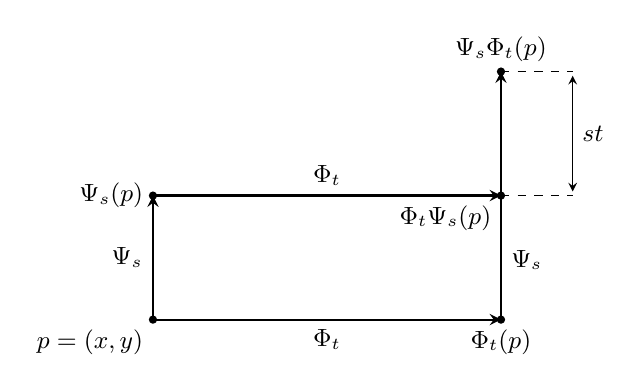
\begin{tikzpicture}[>=stealth,x=1.3cm,y=1.05cm,font=\small]
		\coordinate (P) at (0,0);
		\coordinate (XP) at (3.4,0);
		\coordinate (YP) at (0,1.5);
		\coordinate (XYP) at (3.4,1.5);
		\coordinate (YXP) at (3.4,3);
		\draw[->,thick] (P)--node[below] {\(\Phi_t\)} (XP);
		\draw[->,thick] (P)--node[left] {\(\Psi_s\)} (YP);
		\draw[->,thick] (YP)--node[above] {\(\Phi_t\)} (XYP);
		\draw[->,thick] (XP)--node[right,pos=.24] {\(\Psi_s\)} (YXP);
		\draw[dashed] (XYP)--(4.1,1.5);
		\draw[dashed] (YXP)--(4.1,3);
		\draw[<->] (4.1,1.55)--node[right] {\(st\)} (4.1,2.95);
		\foreach \Q in {P,XP,YP,XYP,YXP} \fill (\Q) circle (1.5pt);
		\node[below left] at (P) {\(p=(x,y)\)};
		\node[below] at (XP) {\(\Phi_t(p)\)};
		\node[left] at (YP) {\(\Psi_s(p)\)};
		\node[below left] at (XYP) {\(\Phi_t\Psi_s(p)\)};
		\node[above] at (YXP) {\(\Psi_s\Phi_t(p)\)};
	\end{tikzpicture}
	\caption{\(X=\partial_x\)、\(Y=x\partial_y\) 的两种运动次序，图中以 \(x,s,t>0\) 示意。先作水平运动会增加随后竖直运动的速度，两个终点的竖直差为 \(st\)。}
	\label{g1:fig:flow-order}
\end{figure}


\subsection{张量场的 Lie 导数}
\label{g1:subsec:1303:03}

流不仅可以搬运向量，也可以搬运度量、形式以及其他张量。\cref{g1:prop:mixed-tensor-pullback}已经说明，微分同胚拉回一个 \((r,s)\) 型张量时，对每个向量因子使用逆微分，对每个对偶因子使用微分的对偶。因此对 \(X\) 的流 \(\Phi\)，
\[
	\bigl((\Phi_t)^*T\bigr)_p
	=\left(\bigl(\mathrm{d}(\Phi_t)_p\bigr)^{-1}\right)^{\otimes r}
	\otimes\left(\bigl(\mathrm{d}(\Phi_t)_p\bigr)^*\right)^{\otimes s}
	\bigl(T_{\Phi_t(p)}\bigr).
\]
这个表达始终位于 \(T^r_s(\mathrm{T}_pM)\)，可以在固定纤维中对时间求导。

\begin{definition}
	\label{g1:def:lie-derivative-tensor}
	设 \(M\) 为无边界光滑流形，\(X\in\mathfrak X(M)\)，\(T\) 为光滑 \((r,s)\) 型张量场。定义 \(T\) 沿 \(X\) 的\term[lidaoshu]{Lie 导数}[Lie derivative]为
	\[
		\mathcal L_XT=\left.\frac{\mathrm{d}}{\mathrm{d}t}\right|_{t=0}(\Phi_t^X)^*T.
	\]
	导数在各点固定的张量纤维中取。局部流对时间和初值光滑，张量拉回的局部公式也光滑，因此这一定义给出同型的光滑张量场。
\end{definition}

在函数上有 \(\mathcal L_Xf=Xf\)，在向量场上有 \(\mathcal L_XY=[X,Y]\)。所以 Lie 导数扩展了同一个沿流比较的想法，无需另选内积或联络；它比较的方式由 \(X\) 的流本身确定。

\begin{proposition}[张量 Lie 导数的计算]
	\label{g1:prop:lie-derivative-tensor-rules}
	设 \(M\) 为无边界光滑流形，\(X\in\mathfrak X(M)\)，\(T,S\) 为光滑张量场，\(f\) 为光滑函数。Lie 导数实线性，并满足
	\[
		\mathcal L_X(T\otimes S)=(\mathcal L_XT)\otimes S+T\otimes(\mathcal L_XS),\qquad
		\mathcal L_X(fT)=X(f)T+f\mathcal L_XT.
	\]
	对任意指定位置的收缩 \(C\)，有 \(\mathcal L_X(CT)=C(\mathcal L_XT)\)。在局部坐标中，
	\begin{equation}
		\label{g1:eq:lie-derivative-tensor-coordinates}
		\begin{split}
			(\mathcal L_XT)^{i_1\cdots i_r}{}_{j_1\cdots j_s}
			={}&\sum_kX^k\partial_kT^{i_1\cdots i_r}{}_{j_1\cdots j_s}\\
			&-\sum_{a=1}^r\sum_k(\partial_kX^{i_a})
			T^{i_1\cdots i_{a-1}k i_{a+1}\cdots i_r}{}_{j_1\cdots j_s}\\
			&+\sum_{b=1}^s\sum_k(\partial_{j_b}X^k)
			T^{i_1\cdots i_r}{}_{j_1\cdots j_{b-1}k j_{b+1}\cdots j_s}.
		\end{split}
	\end{equation}
	此外，在流的共同定义域内，
	\[
		\frac{\mathrm{d}}{\mathrm{d}t}(\Phi_t^X)^*T
		=(\Phi_t^X)^*(\mathcal L_XT)
		=\mathcal L_X\bigl((\Phi_t^X)^*T\bigr).
	\]
	因此 \(\mathcal L_XT=0\) 当且仅当 \(T\) 被 \(X\) 的局部流保持。
\end{proposition}
\begin{proof}
	拉回保持张量积与收缩，见\cref{g1:prop:mixed-tensor-pullback}。对这些恒等式在 \(t=0\) 求导，用通常的乘积求导法则，便得到前两条乘法公式及收缩相容性。它也保持因子的排列，因此对称张量和交替张量的 Lie 导数仍保持各自的对称性。

	为得到坐标公式，先计算坐标基及对偶基的导数。向量场情形已知
	\[
		\mathcal L_X\partial_i=[X,\partial_i]=-\sum_k(\partial_iX^k)\partial_k.
	\]
	对任意一形式 \(\alpha\) 与向量场 \(Y\)，拉回和求值相容：
	\[
		(\Phi_t)^*(\alpha(Y))=((\Phi_t)^*\alpha)((\Phi_t)^*Y).
	\]
	在零时刻求导，得到
	\begin{equation}
		\label{g1:eq:lie-one-form-evaluation}
		(\mathcal L_X\alpha)(Y)=X(\alpha(Y))-\alpha([X,Y]).
	\end{equation}
	令 \(\alpha=\mathrm{d}x^j\)、\(Y=\partial_i\)，由于 \(\mathrm{d}x^j(\partial_i)=\delta_i^j\) 为常数，便有
	\[
		\mathcal L_X(\mathrm{d}x^j)=\sum_i(\partial_iX^j)\,\mathrm{d}x^i.
	\]
	将 \(T\) 在坐标张量基中展开，分别对系数、每个向量基因子及每个对偶基因子求导，就得到\eqref{g1:eq:lie-derivative-tensor-coordinates}。上指标的负号来自向量基的导数，下指标的正号来自对偶基的导数。

	最后，与\cref{g1:prop:flow-pullback-derivative}的证明一样，在一个共同定义的邻域中分别用
	\[
		(\Phi_{t+h})^*=(\Phi_t)^*(\Phi_h)^*
		=(\Phi_h)^*(\Phi_t)^*
	\]
	对 \(h\) 在零处求导，得到一般时间的两个等式。若 \(\mathcal L_XT=0\)，固定 \(p\) 后，\(\bigl((\Phi_t)^*T\bigr)_p\) 在固定有限维张量空间中导数为零，故等于 \(T_p\)；反向只需在 \(t=0\) 求导。
\end{proof}

同样对一般求值恒等式求导，可以得到一个无需坐标的计算方法。若 \(T\) 为协变 \(k\) 阶张量，则
\begin{equation}
	\label{g1:eq:lie-covariant-evaluation}
	(\mathcal L_XT)(Y_1,\ldots,Y_k)
	=X\bigl(T(Y_1,\ldots,Y_k)\bigr)
	-\sum_{a=1}^kT(Y_1,\ldots,[X,Y_a],\ldots,Y_k).
\end{equation}
右端第一项对整个实值函数求导，后面的各项扣除输入向量场随流变化的影响。对混合张量，还要对每个协变向量输入扣除对应的 \(\mathcal L_X\alpha\) 项；这由相同的求值乘积法则得到。只保留第一个方向导数而省略输入的修正，一般不会得到张量运算。

\begin{example}[膨胀下的张量变化]
	\label{g1:exm:lie-dilation-tensors}
	在 \(\mathbb R^n\) 上令 \(X=\sum_i x^i\partial_i\)，其流为 \(\Phi_t(x)=e^t x\)。常向量场和坐标一形式的拉回分别满足
	\[
		(\Phi_t)^*\partial_i=e^{-t}\partial_i,\qquad
		(\Phi_t)^*(\mathrm{d}x^i)=e^t\,\mathrm{d}x^i.
	\]
	所以 \(\mathcal L_X\partial_i=-\partial_i\)，而 \(\mathcal L_X(\mathrm{d}x^i)=\mathrm{d}x^i\)。Euclid 内积与标准最高次形式因而满足
	\[
		\mathcal L_X\left(\sum_i\mathrm{d}x^i\otimes\mathrm{d}x^i\right)
		=2\sum_i\mathrm{d}x^i\otimes\mathrm{d}x^i,\qquad
		\mathcal L_X(\mathrm{d}x^1\wedge\cdots\wedge\mathrm{d}x^n)
		=n\,\mathrm{d}x^1\wedge\cdots\wedge\mathrm{d}x^n.
	\]
	这些张量的坐标系数都是常数，Lie 导数却不为零，因为膨胀会改变向量输入的尺度。相反，对任意常数倍平移场，流的微分是恒等映射，这些常系数张量的 Lie 导数为零。
\end{example}

\subsection{自然性及分次 Cartan 运算的准备}
\label{g1:subsec:1303:04}

讨论映射与 Lie 括号的相容性时，不能沿任意光滑映射直接“推出一个向量场”。微分确实把单个切向量向前送，但同一目标点可能有多个原像，得到的向量未必一致；也可能目标方向根本不在微分的像中。需要明确要求两边的场彼此对应。

\begin{definition}
	\label{g1:def:related-vector-fields}
	设 \(F:M\to N\) 为无边界光滑流形之间的光滑映射。若 \(X\in\mathfrak X(M)\)、\(\overline X\in\mathfrak X(N)\) 满足
	\[
		\mathrm{d}F_pX_p=\overline X_{F(p)}\qquad(p\in M),
	\]
	称它们为 \(F\)-\term[xiangguanxiangliangchang]{相关向量场}[related vector fields]。
\end{definition}

由\cref{g1:def:manifold-differential}，相关条件等价于对目标上的每个局部光滑函数 \(f\) 有
\[
	X(f\circ F)=(\overline Xf)\circ F.
\]
反向也成立，因为将这一等式用于目标坐标函数，就能逐分量确定两个目标切向量相等。因此相关条件可以用函数检验，无需给 \(F\) 额外的可逆性。

\begin{proposition}[Lie 导数的自然性]
	\label{g1:prop:lie-derivative-natural}
	设 \(F:M\to N\) 为无边界光滑流形之间的光滑映射，\(X,\overline X\) 为 \(F\)-相关向量场。
	\begin{enumerate}
		\item 若 \(Y,\overline Y\) 也 \(F\)-相关，则 \([X,Y]\) 与 \([\overline X,\overline Y]\) \(F\)-相关。
		\item 记 \(X,\overline X\) 的局部流为 \(\Phi,\overline\Phi\)，则在每个初始点附近的充分小共同时间内，
		\[
			F\circ\Phi_t=\overline\Phi_t\circ F.
		\]
		\item 对 \(N\) 上任意光滑协变张量 \(T\)，有
		\[
			\mathcal L_X(F^*T)=F^*(\mathcal L_{\overline X}T).
		\]
		若 \(F\) 为局部微分同胚，同式也适用于任意混合张量。对任意微分形式 \(\alpha\)，无须可逆性即有
		\[
			\iota_X(F^*\alpha)=F^*(\iota_{\overline X}\alpha).
		\]
	\end{enumerate}
\end{proposition}
\begin{proof}
	对任意目标局部函数 \(f\)，连续使用相关条件可得
	\[
		\begin{aligned}
			[X,Y](f\circ F)
			&=X\bigl((\overline Yf)\circ F\bigr)
			-Y\bigl((\overline Xf)\circ F\bigr)\\
			&=(\overline X\overline Yf-\overline Y\overline Xf)\circ F
			=([\overline X,\overline Y]f)\circ F.
		\end{aligned}
	\]
	由函数检验条件得到第一项。这里既没有使用单射性，也没有使用满射性。

	对固定 \(p\)，曲线 \(t\mapsto F(\Phi_t(p))\) 的导数为
	\[
		\mathrm{d}F_{\Phi_t(p)}X_{\Phi_t(p)}
		=\overline X_{F(\Phi_t(p))},
	\]
	初值为 \(F(p)\)。它与 \(t\mapsto\overline\Phi_t(F(p))\) 满足同一初值问题，故在共同时间内相同。局部流的开定义域和连续性允许在 \(p\) 的一个邻域中同时选取充分小的时间区间，得到第二项的局部映射恒等式。

	协变张量的拉回始终有定义，并与复合相容，见\cref{g1:prop:covariant-tensor-pullback}。将第二项拉回，得到
	\[
		\Phi_t^*(F^*T)=F^*(\overline\Phi_t^*T).
	\]
	对 \(t\) 在零处求导，得到第三项的 Lie 导数公式。右边的 \(F^*\) 由固定的微分 \(\mathrm{d}F\) 作用于各输入，局部表达是固定系数与张量分量的有限次乘法和求和，所以求导可以穿过它。若 \(F\) 为局部微分同胚，各微分可逆，\cref{g1:prop:mixed-tensor-pullback}使同一个论证也适用于混合张量。

	最后，对任意 \(v_1,\ldots,v_{k-1}\in \mathrm{T}_pM\)，有
	\[
		\begin{aligned}
			\bigl(\iota_XF^*\alpha\bigr)_p(v_1,\ldots,v_{k-1})
			&=\alpha_{F(p)}(\mathrm{d}F_pX_p,\mathrm{d}F_pv_1,\ldots,\mathrm{d}F_pv_{k-1})\\
			&=\alpha_{F(p)}(\overline X_{F(p)},\mathrm{d}F_pv_1,\ldots,\mathrm{d}F_pv_{k-1}),
		\end{aligned}
	\]
	恰为右端的值。零次形式时两边均为零。
\end{proof}

若 \(F\) 是微分同胚，可以定义目标向量场
\[
	(F_*X)_q=\mathrm{d}F_{F^{-1}(q)}X_{F^{-1}(q)}.
\]
此时相关性自动成立，命题给出 \(F_*[X,Y]=[F_*X,F_*Y]\)。但对于投影 \(P(x,y)=x\)，向量场 \(y\partial_x\) 在不同原像 \((x,y)\) 上会送出不同的目标速度，因此没有与它相关的目标向量场。自然性命题的假设不能由“映射光滑”代替。

\ProseParagraphBreak

最后整理微分形式上的两个运算。\(\mathcal L_X\) 保持形式次数，\(\iota_X\) 将次数降低 \(1\)，并在函数上取零。\cref{g1:prop:interior-product-rule}已经证明
\[
	\iota_X(\alpha\wedge\beta)
	=(\iota_X\alpha)\wedge\beta+(-1)^p\alpha\wedge(\iota_X\beta),
	\qquad \alpha\in\Omega^p(M).
\]
符号来自将被插入的向量越过前面 \(p\) 个输入位置。把这类带次数的运算放在一起时，合适的交换子是
\[
	[A,B]_{\mathrm{gr}}=A\circ B-(-1)^{ab}B\circ A,
\]
其中 \(a,b\) 是各自改变形式次数的数。这称为分次交换子；两个次数为 \(-1\) 的运算之间对应的是反交换和，而不是普通差。

\begin{proposition}[插入与 Lie 导数]
	\label{g1:prop:cartan-insertion-identities}
	设 \(M\) 为无边界光滑流形，\(X,Y\in\mathfrak X(M)\)，\(\alpha,\beta\) 为微分形式。则
	\[
		\mathcal L_X(\alpha\wedge\beta)
		=(\mathcal L_X\alpha)\wedge\beta+\alpha\wedge(\mathcal L_X\beta),
	\]
	并且
	\begin{align*}
		\iota_X\iota_Y+\iota_Y\iota_X&=0,\\
		\mathcal L_X\iota_Y-\iota_Y\mathcal L_X&=\iota_{[X,Y]},\\
		\mathcal L_X\mathcal L_Y-\mathcal L_Y\mathcal L_X&=\mathcal L_{[X,Y]}.
	\end{align*}
	最后一式也适用于任意混合张量场。
\end{proposition}
\begin{proof}
	拉回保持楔积，故对 \(\Phi_t^*(\alpha\wedge\beta)=\Phi_t^*\alpha\wedge\Phi_t^*\beta\) 在零时刻求导，得到第一式。Lie 导数的次数是零，因此第二项前没有额外的分次符号。

	对至少二次的形式 \(\alpha\)，先插入 \(Y\)，再插入 \(X\)，得到
	\[
		(\iota_X\iota_Y\alpha)(v_1,\ldots)=\alpha(Y,X,v_1,\ldots).
	\]
	反向次序给出 \(\alpha(X,Y,v_1,\ldots)\)，由交替性二者相加为零。次数为零或一时，两次插入都给出零，因此第一条交换关系对所有次数成立。

	取 \(X\) 的局部流 \(\Phi\)。\cref{g1:prop:lie-derivative-natural}的插入相容性用于微分同胚 \(\Phi_t\)，其中源向量场是 \(\Phi_t^*Y\)，得到
	\[
		\Phi_t^*(\iota_Y\alpha)
		=\iota_{\Phi_t^*Y}(\Phi_t^*\alpha).
	\]
	插入对向量场和形式各自线性，且逐点为双线性运算。对右端用乘积求导法则，并用 \(\left.\partial_t\right|_0\Phi_t^*Y=[X,Y]\)，便得
	\[
		\mathcal L_X(\iota_Y\alpha)
		=\iota_{[X,Y]}\alpha+\iota_Y(\mathcal L_X\alpha),
	\]
	这就是第二条交换关系。

	为证明最后一条，记 \(D=\mathcal L_X\mathcal L_Y-\mathcal L_Y\mathcal L_X-\mathcal L_{[X,Y]}\)。两个次数为零的张量积导子的交换子仍是张量积导子：将它作用于 \(T\otimes S\)，展开后交叉项 \((\mathcal L_XT)\otimes(\mathcal L_YS)\) 与 \((\mathcal L_YT)\otimes(\mathcal L_XS)\) 分别抵消，余下的正是两端各自求导之和。因此 \(D\) 是张量积导子，并且与收缩相容。

	在函数上，\(Df=XYf-YXf-[X,Y]f=0\)。在向量场 \(Z\) 上，由 Jacobi 恒等式，
	\[
		DZ=[X,[Y,Z]]-[Y,[X,Z]]-[[X,Y],Z]=0.
	\]
	对任意一形式 \(\eta\) 与局部向量场 \(Z\)，求值是张量积之后的收缩，所以
	\[
		0=D(\eta(Z))=(D\eta)(Z)+\eta(DZ)=(D\eta)(Z).
	\]
	取坐标向量场逐个检验，得到 \(D\eta=0\)。任意张量在局部都是光滑函数乘若干向量场与一形式的张量积之和，导子法则遂给出 \(DT=0\)。这证明了所有混合张量上的最后一式，形式情形包含在其中。
\end{proof}

这些等式把运动、插入和交替性联系起来。在\secref{g1:sec:1401}中，将构造把形式次数提高 \(1\) 的外微分 \(\mathrm{d}\)，并证明 Cartan 公式\footnote{Cartan，Élie Joseph Cartan（1869--1951），法国数学家，研究 Lie 群、Lie 代数与微分几何，发展了活动标架方法。}
\[
	\mathcal L_X=\mathrm{d}\iota_X+\iota_X\mathrm{d}.
\]
这里的加号与两个奇次数运算的分次交换子相符；定义外微分以后，将给出该公式及其证明。
% 纲要条目排为编号小节标题，并进入目录与书签；说明段仍保留于纲要注释中。

% !TeX root = ../../Book1.tex
% 纲要标题：### 13.4 Frobenius 定理与积分叶
% 纲要位置：几何学计划纲要.md，第 627 行。
% 正文状态：初稿；尚未正式审核。

% 纲要内容开始
% 
% * 分布、局部标架与积分流形
% * 对合条件的必要性
% * 对合分布的交换化标架
% * 适应坐标和局部积分叶的构造
% * 最大连通积分叶及唯一性
% 
% 纲要内容结束

\section{Frobenius 定理与积分叶}
\label{g1:sec:1304}

给定一条非零向量场，可以沿其积分曲线组织局部坐标。如果在每一点指定的是一个 \(r\) 维切平面，能否找到 \(r\) 维子流形，使它在各点的切空间恰好等于所指定的平面？这里的困难不只是分别沿 \(r\) 个方向求积分曲线：先沿一个方向、再沿另一个方向移动，可能产生离开原平面的额外方向。Lie 括号正好测量这种不相容性。

\ProseParagraphBreak

本节始终在有限维、Hausdorff、第二可数且无边界的光滑流形上讨论常秩光滑分布。证明先把对合分布的局部标架换成两两交换的标架，再用交换流构造坐标。局部坐标片的粘合会给出最大连通积分叶；叶片的粘合还将赋予叶自身的拓扑，并保证 Hausdorff 性和第二可数性。

\subsection{分布、局部标架与积分流形}
\label{g1:subsec:1304:01}

\begin{definition}[光滑分布]\label{g1:def:smooth-distribution}
	设 \(M^n\) 为无边界光滑流形，\(0\le r\le n\)。切丛 \(\mathrm{T}M\) 的秩 \(r\) 光滑向量子丛 \(D\subseteq \mathrm{T}M\) 称为一个秩 \(r\) 的\term[guanghuafenbu]{光滑分布}[smooth distribution]。等价地，在每个 \(p\in M\) 的某邻域 \(U\) 上，存在光滑向量场 \(Z_1,\ldots,Z_r\)，使它们在每一点线性无关，且
	\[
		D_q=\operatorname{span}\{Z_1(q),\ldots,Z_r(q)\}\qquad(q\in U).
	\]
	这样的向量场组称为 \(D\) 的局部标架。记 \(\Gamma(U,D)\) 为 \(U\) 上所有取值于 \(D\) 的光滑向量场。
\end{definition}

这个等价描述正是\cref{g1:def:vector-subbundle}对 \(\mathrm{T}M\) 的应用。固定维数还不够，局部标架的光滑性也属于条件。另一方面，“取值于 \(D\) 的光滑向量场”确实是子丛的光滑截面：由\cref{g1:prop:subbundle-adapted-frame}把局部标架补成 \(\mathrm{T}M\) 的标架后，后面的分量恒为零，前面的分量仍光滑。因而任意 \(X\in\Gamma(U,D)\) 都唯一写为
\[
	X=\sum_{i=1}^r f^iZ_i
\]
且各 \(f^i\) 光滑。

\begin{definition}[积分流形]\label{g1:def:integral-manifold}
	设 \(D\subseteq \mathrm{T}M\) 为秩 \(r\) 光滑分布。一个 \(r\) 维无边界光滑流形 \(N\)，连同单射浸入 \(\iota:N\to M\)，若满足
	\[
		\mathrm{d}\iota_q(\mathrm{T}_qN)=D_{\iota(q)}\qquad(q\in N),
	\]
	则称为 \(D\) 的一个\term[jifenliuxing]{积分流形}[integral manifold]。把 \(N\) 与其像识别时，像使用从 \(N\) 搬来的流形拓扑和光滑结构，不预先要求它们等于子空间拓扑及嵌入子流形结构。若每个 \(p\in M\) 都位于某个积分流形的像内，则称 \(D\) 可积。
\end{definition}

这里单射使一个像点只有一个参数点，浸入则保证局部参数确实给出一块 \(r\) 维曲面。然而，\cref{g1:exm:injective-immersion-not-embedding}已经说明，单射浸入未必是嵌入：可能有环境空间中相近的点，在参数流形中相距很远。因此积分流形的拓扑可以比像的子空间拓扑更细。后面构造最大叶时，会明确选出这个拓扑。

\begin{example}\label{g1:exm:submersion-integral-levels}
	若 \(F:M^n\to N^{n-r}\) 是光滑淹没，则 \(D=\ker\mathrm{d}F\) 为秩 \(r\) 光滑分布。其子丛性质来自\cref{g1:thm:constant-rank-bundle-morphism}：把 \(\mathrm{d}F\) 看成 \(\mathrm{T}M\to F^*\mathrm{T}N\) 的满射丛同态，其核秩恒为 \(r\)。对每个非空水平集 \(F^{-1}(y)\)，\cref{g1:thm:regular-level-set}给出嵌入子流形结构，且
	\[
		\mathrm{T}_pF^{-1}(y)=\ker\mathrm{d}F_p=D_p.
	\]
	因此水平集及其连通分支都是积分流形。在这个例子中，积分流形由一些保持不变的函数值刻画；\term[frobeniusdingli]{Frobenius 定理}[Frobenius theorem]\footnote{Frobenius，Ferdinand Georg Frobenius（1849--1917），德国数学家，研究群的表示与特征标以及微分方程。}将证明，对合条件正好保证局部总能找到这样的横向坐标函数。
\end{example}

秩零分布的连通积分流形是单点；秩 \(n\) 的分布只能是 \(\mathrm{T}M\)，其局部积分流形是开集。以下证明也包含这两个情形，空的标架或横向坐标按通常的零维约定理解。

\subsection{对合条件的必要性}
\label{g1:subsec:1304:02}

若两条向量场都沿同一个积分流形运动，它们的无穷小交换也应当沿这个流形。为把这个直观判断写成坐标无关的条件，我们使用\cref{g1:def:lie-bracket}中的括号
\[
	[X,Y]f=X(Yf)-Y(Xf).
\]

\begin{definition}[对合分布]\label{g1:def:involutive-distribution}
	设 \(D\subseteq \mathrm{T}M\) 为光滑分布。若对任意开集 \(U\subseteq M\) 及任意 \(X,Y\in\Gamma(U,D)\)，都有
	\[
		[X,Y]\in\Gamma(U,D),
	\]
	则称 \(D\) 为\term[duihefenbu]{对合分布}[involutive distribution]。
\end{definition}

检查对合性时，只需检查一组局部标架的两两括号。事实上，由\cref{g1:prop:lie-bracket-properties}的乘积法则，
\[
	\left[\sum_i f^iZ_i,\sum_j g^jZ_j\right]
	=\sum_{i,j}f^ig^j[Z_i,Z_j]
	+\sum_{i,j}f^iZ_i(g^j)Z_j
	-\sum_{i,j}g^jZ_j(f^i)Z_i.
\]
后两项自动取值于 \(D\)，第一项则由标架括号条件控制。对合不要求原标架彼此交换。例如 \(\mathrm{T}\mathbb R^2\) 的标架 \(\partial_x,e^x\partial_y\) 满足 \([\partial_x,e^x\partial_y]=e^x\partial_y\ne0\)，但括号仍在该分布中。秩一分布自动对合，因为 \([fX,gX]=(fXg-gXf)X\)。

\begin{proposition}[可积性的必要条件]\label{g1:prop:involutivity-necessary}
	设 \(M\) 为无边界光滑流形，\(D\subseteq \mathrm{T}M\) 为常秩光滑分布。若每个点都有通过它的积分流形，则 \(D\) 对合。更具体地，若 \(\iota:N\to M\) 是一个积分流形，\(X,Y\) 为某开集 \(U\) 上取值于 \(D\) 的光滑向量场，则 \([X,Y]\) 在 \(U\cap\iota(N)\) 上也取值于 \(D\)。
\end{proposition}
\begin{proof}
	在 \(\iota^{-1}(U)\) 上，因 \(\mathrm{d}\iota_q:\mathrm{T}_qN\to D_{\iota(q)}\) 为线性同构，可唯一定义向量场 \(\widetilde X,\widetilde Y\)，使
	\[
		\mathrm{d}\iota\,\widetilde X=X\circ\iota,\qquad
		\mathrm{d}\iota\,\widetilde Y=Y\circ\iota.
	\]
	它们光滑。具体地，在局部标架中，\(\mathrm{d}\iota\) 给出到拉回分布 \(\iota^*D\) 的光滑可逆矩阵；其逆由伴随矩阵除以非零行列式给出，故光滑，正如\cref{g1:prop:bundle-morphism-matrices}所述。

	相关向量场的括号仍相关，见\cref{g1:prop:lie-derivative-natural}。当前所用的计算很短：对 \(f\in C^\infty(U)\)，有
	\[
		\begin{aligned}
			[\widetilde X,\widetilde Y](f\circ\iota)
			&=\widetilde X\bigl((Yf)\circ\iota\bigr)-\widetilde Y\bigl((Xf)\circ\iota\bigr)\\
			&=([X,Y]f)\circ\iota.
		\end{aligned}
	\]
	以导子判断切向量，得到
	\[
		[X,Y]_{\iota(q)}
		=\mathrm{d}\iota_q\bigl([\widetilde X,\widetilde Y]_q\bigr)
		\in \mathrm{d}\iota_q(\mathrm{T}_qN)=D_{\iota(q)}.
	\]
	若每个点都有这样的积分流形，就在每一点得到所需的包含关系，故 \([X,Y]\) 为 \(D\) 的光滑截面。
\end{proof}

浸入微分把 \(\mathrm{T}N\) 同构到沿像的 \(D\)，因而能将局部的分布截面提升到积分流形；括号自然性随后把它们的括号送回 \(D\)。

\subsection{对合分布的交换化标架}
\label{g1:subsec:1304:03}

对合条件只说 \([Z_i,Z_j]\) 能用原标架线性表示，而交换流需要的是括号等于零。关键在于先选择若干坐标方向，使它们在 \(D\) 上能够独立测量所有分量，再把这些分量归一化。这样新标架的括号既必须留在 \(D\)，又失去了在这些方向上的全部分量，只能为零。

\begin{lemma}[交换化分布标架]\label{g1:lem:commuting-distribution-frame}
	设 \(D\) 为无边界光滑流形 \(M^n\) 上的秩 \(r\) 对合光滑分布。对每个 \(p\in M\)，存在以 \(p\) 为原点的坐标
	\[
		(x^1,\ldots,x^r,y^1,\ldots,y^{n-r})
	\]
	及 \(D\) 的光滑局部标架 \(X_1,\ldots,X_r\)，满足
	\begin{equation}\label{g1:eq:normalized-distribution-frame}
		X_i=\frac{\partial}{\partial x^i}
		+\sum_{\alpha=1}^{n-r}a_i^\alpha(x,y)\frac{\partial}{\partial y^\alpha},
		\qquad [X_i,X_j]=0.
	\end{equation}
\end{lemma}
\begin{proof}
	先取任意局部标架 \(Z_1,\ldots,Z_r\) 和环境坐标 \(z^1,\ldots,z^n\)。在 \(p\) 处，系数矩阵 \((Z_jz^a)_{a,j}\) 的秩为 \(r\)，所以有一个非零的 \(r\) 阶子式。重排坐标后，可令它由前 \(r\) 行给出，记这部分坐标为 \(x\)，其余为 \(y\)。缩小邻域使
	\[
		B_{aj}=Z_jx^a\qquad(1\le a,j\le r)
	\]
	始终可逆，并定义
	\[
		X_i=\sum_{j=1}^r(B^{-1})_{ji}Z_j.
	\]
	逆矩阵光滑，新向量场仍为 \(D\) 的标架；并且
	\[
		X_ix^a=\sum_jB_{aj}(B^{-1})_{ji}=\delta_i^a.
	\]
	这就给出\eqref{g1:eq:normalized-distribution-frame}中的第一式。

	投影到前 \(r\) 个坐标的微分 \(\mathrm{d}x:D_q\to\mathbb R^r\) 在整个邻域中为同构，因为它把 \(X_i(q)\) 送到第 \(i\) 个标准基向量。另一方面，
	\[
		[X_i,X_j]x^a=X_i(\delta_j^a)-X_j(\delta_i^a)=0.
	\]
	所以括号的全部 \(x\) 分量为零。同时，对合性使它属于 \(D_q\)。一个属于 \(D_q\) 且被 \(\mathrm{d}x\) 送到零的向量只能为零，故 \([X_i,X_j]=0\)。
\end{proof}

这一步只换了分布的标架，还没有找到使 \(X_i\) 本身成为坐标向量的坐标。后一任务由流完成。若直接展开刚才消失的横向分量，还可把对合条件写为
\[
	\partial_{x^i}a_j^\alpha-\partial_{x^j}a_i^\alpha
	+\sum_{\beta=1}^{n-r}\left(
		a_i^\beta\partial_{y^\beta}a_j^\alpha
		-a_j^\beta\partial_{y^\beta}a_i^\alpha
	\right)=0.
\]
这些是系数之间的相容方程；不必另外求解这组偏微分方程，交换的局部流会直接给出积分片。

\subsection{适应坐标和局部积分叶的构造}
\label{g1:subsec:1304:04}

交换化标架给出沿各个允许方向的交换流。把这些流依次作用在一张横向小截面上，流时间与截面坐标便组成候选坐标；逆函数定理将证明它们确实覆盖一个邻域。

\begin{theorem}[Frobenius 定理]\label{g1:thm:frobenius}
	设 \(M^n\) 为有限维、Hausdorff、第二可数且无边界的光滑流形，\(D\subseteq \mathrm{T}M\) 为秩 \(r\) 光滑分布。下列条件等价：
	\begin{enumerate}
		\item \(D\) 对合；
		\item 每个点附近都有坐标 \((u^1,\ldots,u^r,v^1,\ldots,v^{n-r})\)，使
		\[
			D=\operatorname{span}\left\{\frac{\partial}{\partial u^1},\ldots,\frac{\partial}{\partial u^r}\right\};
		\]
		\item 每个点都位于某个 \(r\) 维积分流形内。
	\end{enumerate}
	第二项中的坐标域可取为乘积 \(B\times T\)，其中 \(B\subseteq\mathbb R^r\)、\(T\subseteq\mathbb R^{n-r}\) 为开球或开盒；固定 \(v=c\) 的切片给出局部嵌入积分流形。
\end{theorem}
\begin{proof}
	设 \(D\) 对合。固定 \(p\)，用\cref{g1:lem:commuting-distribution-frame}取得局部坐标 \((x,y)\) 和两两交换的标架 \(X_1,\ldots,X_r\)。令 \(\Phi_i^t\) 为 \(X_i\) 的局部流。\cref{g1:thm:maximal-local-flow,g1:thm:ode-smooth-dependence}保证它们在零时间附近存在，且对时间与初值联合光滑；不需要这些向量场完备。由\cref{g1:thm:commuting-local-flows}，在足够小的共同邻域内，各局部流两两交换。

	取横截片 \(\sigma(y)=(0,y)\)，定义
	\begin{equation}\label{g1:eq:frobenius-flow-coordinates}
		\Psi(t,y)=\Phi_r^{t^r}\circ\cdots\circ\Phi_1^{t^1}(\sigma(y)).
	\end{equation}
	这时必须使一个参数盒内的全部复合都有定义。因为只有有限条流及交换时所需的有限种复合，零参数时所有中间点都在 \(p\) 附近；各流的定义域开放，故可同时缩小时间盒和横截片，使这些复合及其中间点都留在上述共同邻域。于是 \(\Psi\) 是一个开参数盒上的光滑映射。

	利用交换性，把第 \(i\) 条流移到最外层，便有
	\[
		\Psi(t+s e_i,y)=\Phi_i^s(\Psi(t,y))
	\]
	对充分小的 \(s\) 成立。在 \(s=0\) 求导得到
	\begin{equation}\label{g1:eq:frobenius-pushed-coordinate-fields}
		\mathrm{d}\Psi_{(t,y)}\!\left(\frac{\partial}{\partial t^i}\right)
		=X_i(\Psi(t,y)).
	\end{equation}
	在 \((0,0)\) 处，时间方向的导数为 \(X_i(p)\)，横截方向的导数为原坐标的 \(\partial_{y^\alpha}|_p\)。因此按 \((x,y)\) 排列的导数矩阵为
	\[
		\mathrm{D}\Psi(0,0)=
		\begin{pmatrix}
			I_r&0\\
			A&I_{n-r}
		\end{pmatrix},
		\qquad A_{\alpha i}=a_i^\alpha(p),
	\]
	它可逆。\cref{g1:thm:inverse-function}给出 \(\Psi\) 在原点附近的光滑逆；再把参数域缩小为乘积 \(B\times T\)，其像仍为开集 \(U\)，且 \(\Psi:B\times T\to U\) 为微分同胚。

	取 \((u,v)=\Psi^{-1}\) 为 \(U\) 上的新坐标。\eqref{g1:eq:frobenius-pushed-coordinate-fields}说明原来的 \(X_i\) 正好成为新坐标向量 \(\partial_{u^i}\)，从而得到第二项。秩零时没有流，直接使用原坐标；满秩时横截片是单点，同一个可逆矩阵论证仍成立。

	第二项推出第三项：固定 \(v=c\)，映射 \(u\mapsto\Psi(u,c)\) 是一块嵌入参数片，其微分像正是 \(D\)，故为积分流形。第三项推出第一项已经由\cref{g1:prop:involutivity-necessary}证明。
\end{proof}

在这样的适应坐标中，把 \(U\) 称为一个\term[yezhuangzuobiaohe]{叶状坐标盒}[foliation box]；对 \(c\in T\)，把
\[
	P_c=\Psi(B\times\{c\})
\]
称为该盒的一张\term[yepian]{叶片}[plaque]。叶片是连通的局部嵌入积分流形。这里的“叶片”只指一个盒中的局部切片，后面所说的“叶”则是最大连通积分流形，不宜混用。\cref{g1:fig:frobenius-plaques}中，横向坐标 \(v\) 区分不同叶片，沿 \(D\) 的运动只改变 \(u\)。

% !TeX root = ../Book1.tex
% 一维叶片的二维示意；一般情形由r维切片替代曲线。
\begin{figure}[htbp]
	\centering
	\begin{tikzpicture}[font=\small]
		\begin{scope}
			\node at (1.8,3.45) {参数盒 \(B\times T\)};
			\fill[GeometryBlueLight] (0,0) rectangle (3.6,3);
			\draw[GeometryGray,dashed] (0,0) rectangle (3.6,3);
			\draw[orange!75!black,thick] (1.8,0.25)--(1.8,2.75);
			\foreach \h in {0.65,2.35}{
				\draw[GeometryGray] (0.25,\h)--(3.35,\h);
			}
			\draw[GeometryBlue,very thick,->] (0.25,1.5)--(3.35,1.5);
			\fill[GeometryBlue] (1.8,1.5) circle[radius=2pt];
			\node[above,fill=GeometryBlueLight,inner sep=1.5pt] at (2.75,1.5) {\(v=c\)};
			\node[orange!75!black,above] at (1.8,2.8) {\(u=0\)};
			\draw[->,GeometryGray] (0.25,-0.35)--(3.35,-0.35) node[right] {\(u\)};
			\draw[->,GeometryGray] (-0.35,0.25)--(-0.35,2.8) node[above] {\(v\)};
		\end{scope}
		\draw[->,thick] (4.05,1.5)--(5.35,1.5) node[midway,above] {\(\Psi\)};
		\begin{scope}[xshift=5.8cm]
			\node at (1.8,3.45) {流形中的坐标邻域 \(U\)};
			\fill[GeometryBlueLight] (0,0) rectangle (3.6,3);
			\draw[GeometryGray,dashed] (0,0) rectangle (3.6,3);
			\draw[orange!75!black,thick] (1.8,0.25)--(1.8,2.75);
			\foreach \h in {0.65,2.35}{
				\draw[GeometryGray] (0.25,\h) .. controls (1.1,{\h+0.45}) and (2.5,{\h-0.45}) .. (3.35,\h);
			}
			\draw[GeometryBlue,very thick] (0.25,1.5) .. controls (1.1,1.95) and (2.5,1.05) .. (3.35,1.5);
			\draw[GeometryBlue,thick,->] (2.05,1.44)--(2.7,1.37);
			\fill[GeometryBlue] (1.8,1.5) circle[radius=2pt];
			\node[GeometryBlue,above] at (2.55,1.47) {\(D\)};
			\node[GeometryBlue,right] at (3.4,1.5) {\(P_c\)};
			\node[orange!75!black,above] at (1.8,2.8) {\(\sigma(y)\)};
		\end{scope}
	\end{tikzpicture}
	\caption{一维叶片的二维示意。固定横向坐标的切片经 \(\Psi\) 变成积分叶片 \(P_c\)，橙色线表示横截片，蓝色箭头表示分布方向。高秩情形用 \(r\) 维片替代曲线，横向坐标仍沿片保持不变。}
	\label{g1:fig:frobenius-plaques}
\end{figure}


\begin{lemma}[局部积分叶片的唯一性]\label{g1:lem:local-integral-plaque}
	设 \(M\) 为无边界光滑流形，\(D\) 为其上的秩 \(r\) 光滑分布。设开集 \(U\subset M\) 具有乘积坐标 \((u,v)\in B\times T\)，其中 \(B,T\) 为开球，且 \(D|_U=\operatorname{span}\{\partial_{u^1},\ldots,\partial_{u^r}\}\)。对 \(c\in T\)，以 \(P_c\) 记切片 \(\{(u,c):u\in B\}\) 在 \(U\) 中的原像。若 \(\iota:N\to M\) 是连通积分流形且 \(\iota(N)\subseteq U\)，则 \(v\circ\iota\) 为常值 \(c\)，且
	\[
		\iota:N\longrightarrow P_c
	\]
	是到 \(P_c\) 某开子集的微分同胚。因此，任何两个通过同一点的积分流形，在分别缩小其参数邻域后，像在该点附近一致。
\end{lemma}
\begin{proof}
	由于 \(\mathrm{d}\iota(\mathrm{T}N)=D\)，而每个横向坐标 \(v^\alpha\) 的微分在 \(D\) 上为零，故
	\[
		\mathrm{d}(v^\alpha\circ\iota)=0.
	\]
	光滑函数微分为零时局部常值：在源坐标小球内沿线段使用一元微积分，函数值不变。连通空间上的局部常值函数为常值，因为一个取值的原像及其补集都是开集。因此 \(v\circ\iota=c\)。

	前 \(r\) 个坐标的微分在 \(D\) 上为同构，所以
	\[
		\mathrm{d}(u\circ\iota)_q
		=\mathrm{d}u_{\iota(q)}\circ\mathrm{d}\iota_q:\mathrm{T}_qN\to\mathbb R^r
	\]
	可逆。逆函数定理表明 \(\iota:N\to P_c\) 是局部微分同胚，因此为开映射。它又单射，故是到其像的同胚，局部光滑逆粘合成整体光滑逆，像在 \(P_c\) 中开。

	最后，对两条通过同一点 \(p\) 的积分流形，先各取连通参数邻域，使像落在同一个适应坐标盒中。两者的横向常值都等于 \(v(p)\)，像都是同一 \(P_{v(p)}\) 中含 \(p\) 的开集。取这两个开集的交，再限制各参数邻域，即得到相同的局部像。
\end{proof}

若一条积分流形没有整个落在 \(U\) 内，只能把引理用于其原像 \(\iota^{-1}(U)\) 的各个连通分支。不同分支可以落在同一个坐标盒的不同叶片上。局部唯一性因此不表示一个完整的积分叶与 \(U\) 只能相交一张叶片，也不保证完整积分叶是嵌入的。

\subsection{最大连通积分叶及唯一性}
\label{g1:subsec:1304:05}

沿相交的叶片继续前进，可以把经过一点的所有局部积分片连在一起。首先需要确定哪些点属于同一片最大对象，然后给这个点集一个使各叶片成为开坐标片的拓扑。这个拓扑下，远行后重新靠近原点的部分不必成为原来那一张局部坐标片中的邻近点。

\begin{theorem}[最大连通积分叶]\label{g1:thm:maximal-connected-leaf}
	设 \(M\) 为有限维、Hausdorff、第二可数且无边界的光滑流形，\(D\subseteq \mathrm{T}M\) 为秩 \(r\) 对合光滑分布。对每个 \(p\in M\)，存在唯一的最大连通积分流形 \(L_p\)，其像包含 \(p\)。更精确地，\(L_p\) 是 \(M\) 的一个子集，带有 Hausdorff、第二可数的 \(r\) 维光滑流形结构，包含映射 \(i_p:L_p\hookrightarrow M\) 为浸入，且任何像包含 \(p\) 的连通积分流形 \(\iota:N\to M\) 都唯一分解为
	\[
		N\xrightarrow{\ \widehat\iota\ }L_p\xrightarrow{\ i_p\ }M,
	\]
	其中 \(\widehat\iota\) 是开嵌入。不同的 \(L_p\) 要么相同，要么不交，故它们将 \(M\) 分割成最大连通积分流形。这些最大积分流形称为 \(D\) 的\term[ye]{叶}[leaf]。
\end{theorem}
\begin{proof}
	先取至多可数个叶状坐标盒 \(U_1,U_2,\ldots\) 覆盖 \(M\)。第二可数性保证可以这样取：在一个可数拓扑基中，对每个能包含于某个给定坐标盒的基元素选一个这样的盒；每点附近都有这样的基元素，所以选出的至多可数个盒仍覆盖 \(M\)。记第 \(j\) 个盒的坐标为 \((u_j,v_j)\in B_j\times T_j\)，其叶片记为 \(P_{j,c}\)。

	如果存在有限叶片链
	\[
		P_0,P_1,\ldots,P_k,\qquad
		P_{\ell-1}\cap P_\ell\ne\varnothing,
	\]
	使两点分别位于首尾叶片，就称这两点可由叶片相连。每点属于某叶片，反转链给出对称性，拼接链给出传递性，所以这是等价关系。令 \(L_p\) 为 \(p\) 的等价类。若一个叶片与 \(L_p\) 相交，便可加到相应的有限链末尾，故整个叶片都包含于 \(L_p\)。

	先说明相交叶片的拓扑如何衔接。设 \(P,Q\) 为所选坐标盒中的两张叶片，且 \(z\in P\cap Q\)。在 \(P\) 内取 \(P\cap U_Q\) 中含 \(z\) 的一个小连通开邻域，其中 \(U_Q\) 是含 \(Q\) 的坐标盒。这个邻域是积分流形，像落在 \(U_Q\) 中，由\cref{g1:lem:local-integral-plaque}，它位于通过 \(z\) 的唯一叶片 \(Q\) 内。因此 \(P\cap Q\) 在 \(P\) 中开；交换二者，同样在 \(Q\) 中开。两张叶片坐标之间的转换，是环境坐标转换限制到这些开集后取前 \(r\) 个分量，因而光滑，其逆也光滑。

	给 \(L_p\) 如下拓扑：\(W\subseteq L_p\) 开，当且仅当对每张包含于 \(L_p\) 的上述叶片 \(P\)，交集 \(W\cap P\) 在 \(P\) 中开。刚才的交集性质说明每张 \(P\) 在这个拓扑中开，而且它的诱导拓扑恰好是原来的 Euclid 片拓扑。例如 \(P\) 中任一开集 \(V\) 与其他叶片 \(Q\) 的交，在开集 \(P\cap Q\) 内经光滑坐标转换仍为开集，因此 \(V\) 也是 \(L_p\) 的开集。各叶片坐标遂组成光滑相容图册。包含映射在每个片上就是坐标切片的包含，所以连续、光滑且微分像为 \(D\)。任意两点可在 \(M\) 中用不交开邻域分开，取这些邻域与 \(L_p\) 的交，仍为叶拓扑中的开集，故 \(L_p\) Hausdorff。

	接着验证第二可数性。这不能由“\(L_p\) 是第二可数空间 \(M\) 的子集”推出，因为刚定义的叶拓扑可能比子空间拓扑更细。我们证明这条叶实际只用到可数张叶片。固定一张叶片 \(P\) 以及一个坐标盒 \(U_j\)。集合 \(P\cap U_j\) 是 \(P\) 的开子集，至多有可数个连通分支：在 \(P\) 的 Euclid 坐标中，每个连通分支都是开集，因为每点的小球连通；不同非空分支各含一个不同的有理坐标点，故只有可数个。秩零时开子集至多为单点，结论同样成立。每个分支 \(C\) 是连通积分流形且位于 \(U_j\) 内，由局部唯一性，\(v_j|_C\) 常值，故 \(C\) 只遇到 \(U_j\) 中的一张叶片。因此对固定的 \(P,U_j\)，与 \(P\) 相交的 \(U_j\) 叶片至多可数。

	坐标盒本来只有可数个，故与固定 \(P\) 相交的全部所选叶片至多可数。现在从一张含 \(p\) 的叶片开始：第一步加入所有与它相交的叶片，第二步加入所有与第一步叶片相交的叶片，依此继续。每一步得到可数集合，可数步之并仍可数，并且恰好包含所有能用有限链从 \(p\) 到达的叶片。它们覆盖 \(L_p\)。每张叶片取一个可数 Euclid 拓扑基，所有这些基的并给出 \(L_p\) 的可数基，因为叶片是开坐标片。至此，\(L_p\) 确实是通常意义下的 Hausdorff、第二可数光滑流形。

	每张叶片同胚于开球或开盒，所以可以在片内用光滑路径连接两点。沿任一有限叶片链选择相邻交点并连接这些路径，得到叶内的连续分片光滑路径。因此 \(L_p\) 路径连通，尤其连通。

	最后证明最大性与唯一性。设 \(\iota:N\to M\) 为连通积分流形，且像包含 \(p\)。对任意 \(q\in N\)，选一个连通参数邻域，其像落在某个 \(U_j\) 内。局部唯一性说明这个像落在一张叶片中，所以 \(N\) 中映入同一叶片等价类的点构成开集；这些开集两两不交并覆盖 \(N\)。由连通性只有一个非空类，且它是 \(L_p\)。故 \(\iota\) 在集合意义下唯一地分解为 \(\widehat\iota:N\to L_p\)。

	在刚才的每个小参数邻域内，\(\widehat\iota\) 的像位于一张开叶片中，而\cref{g1:lem:local-integral-plaque}使它成为到该叶片开子集的微分同胚。因此 \(\widehat\iota\) 是局部微分同胚，特别地连续且开。它由 \(\iota\) 的单射性而单射，故为开嵌入。这证明 \(L_p\) 包含经过 \(p\) 的每个连通积分流形的像。任何另一个最大连通积分流形必须具有相同的像，两个结构之间的恒等映射又由上述分解在两个方向光滑，所以最大对象连同流形结构都唯一。最后，等价类本来相同或不交，故叶构成 \(M\) 的分割。
\end{proof}

这个由最大叶组成的分割，连同上述局部乘积坐标，称为 \(M\) 上的一个 \(r\) 维\term[yezhuangjiegou]{光滑叶状结构}[smooth foliation]，常记为 \(\mathcal F\)。各叶在每个坐标盒中分解为若干叶片；叶片之间的切向空间相容，合起来正是原来的分布 \(D\)。

\ProseParagraphBreak

这个证明同时给出了叶状坐标盒的内在用途：它们既提供叶的局部图，又用可数传播控制叶的整体拓扑。对任一固定盒，一条叶可能经过可数多张不同叶片，而不是只有一张；叶中的邻近由单张叶片上的坐标决定，环境中的再次靠近则未必意味着叶内的靠近。

\ProseParagraphBreak

Frobenius 定理由常秩、光滑性与对合条件得到局部适应坐标，并得到具有自身流形结构的最大连通叶。叶是否嵌入、压缩各叶所得商空间是否 Hausdorff，则取决于叶离开局部坐标盒后的整体行为。下一节将在环面流和横截面返回的模型中计算这些行为。

% 纲要条目排为编号小节标题，并进入目录与书签；说明段仍保留于纲要注释中。

% !TeX root = ../../Book1.tex
% 纲要标题：### 13.5 叶状结构的整体问题与不可积模型
% 纲要位置：几何学计划纲要.md，第 635 行。
% 正文状态：初稿；尚未正式审核。

% 纲要内容开始
% 
% * 环面上的有理和无理斜率叶
% * 横截面、返回映射及沿叶映射芽
% * 非 Hausdorff 叶空间
% * 标准接触分布的不可积性
% 
% ---
% 
% 纲要内容结束

\section{叶状结构的整体问题与不可积模型}
\label{g1:sec:1305}

Frobenius 定理给每个点附近一叠坐标切片，最大叶定理则说明怎样沿这些切片继续前进。继续以后会发生什么，仍须另外研究：一条叶可能闭合，也可能反复进入同一个坐标盒，甚至在整个流形中稠密；沿叶绕一圈后，邻近叶的横向位置也可能改变。本节用几个能够直接计算的模型分辨这些现象。全节的流形均无边界，分布均为常秩光滑分布。

\subsection{环面上的有理和无理斜率叶}
\label{g1:subsec:1305:01}

把二维环面写为 \(T^2=\mathbb R^2/\mathbb Z^2\)，即分别把两个坐标模 \(1\) 识别。局部坐标来自小矩形的商像，换坐标只是整数平移，所以常向量场
\[
	X_\alpha=\partial_x+\alpha\partial_y,\qquad \alpha\in\mathbb R,
\]
下降为环面上的处处非零光滑向量场。它的流为
\[
	\Phi_t([x,y])=[x+t,y+\alpha t].
\]
这给出一个处处秩一的分布 \(D_\alpha=\mathbb RX_\alpha\)。秩一分布总对合，因为 \([fX_\alpha,gX_\alpha]=(fX_\alpha g-gX_\alpha f)X_\alpha\)；由\cref{g1:thm:maximal-connected-leaf}，其叶就是这些流轨道，带上各自的积分流形拓扑。

\begin{proposition}[环面上的线性叶]
	\label{g1:prop:linear-torus-leaves}
	设 \(T^2=\mathbb R^2/\mathbb Z^2\)，\(\alpha\in\mathbb R\)，\(X_\alpha=\partial_x+\alpha\partial_y\)，\(D_\alpha=\mathbb R X_\alpha\)，其流为 \(\Phi_t([x,y])=[x+t,y+\alpha t]\)。若 \(\alpha=p/q\)，其中 \(p\in\mathbb Z\)、\(q\in\mathbb Z_{\geq1}\) 且 \(\gcd(p,q)=1\)，则每条 \(D_\alpha\) 叶为嵌入圆周，最小正流周期为 \(q\)。若 \(\alpha\) 无理，则每条叶为 \(\mathbb R\) 的单射浸入像，在整个环面中稠密，且不是嵌入子流形。
\end{proposition}
\begin{proof}
	轨道在时刻 \(t\) 返回初始点，当且仅当 \(t\in\mathbb Z\) 且 \(\alpha t\in\mathbb Z\)。有理情形中这等价于 \(t\in q\mathbb Z\)。于是轨道参数化下降为单射浸入 \(\mathbb R/q\mathbb Z\to T^2\)。定义域紧而目标 Hausdorff，所以它到像为同胚，结合浸入性即为光滑嵌入。

	无理情形没有非零返回时间，故轨道参数化 \(\mathbb R\to T^2\) 单射，其微分是处处非零的 \(X_\alpha\)，因此是浸入。先证明整数倍 \(\{n\alpha\bmod1:n\in\mathbb Z\}\) 在圆周稠密。将 \(0,\alpha,\ldots,N\alpha\) 的小数部分放入 \(N\) 个等长区间，至少两点落在同一段。两者之差取适当正负号，就得到某个非零整数 \(k\) 及整数 \(m\)，使
	\[
		0<\delta=k\alpha-m<\frac1N.
	\]
	各数 \(0,\delta,\ldots,\lfloor1/\delta\rfloor\delta\) 都来自整数倍 \(\alpha\) 模 \(1\)，并且与 \([0,1]\) 中任一点的距离不超过 \(\delta\)。令 \(N\) 任意大，便得稠密性。对环面中任意小开矩形，先固定其中一个第一坐标 \(u\)。轨道在时刻 \(t=u-x_0+n\) 的第一坐标均为 \(u\) 模 \(1\)，第二坐标为
	\[
		y_0+\alpha(u-x_0)+n\alpha\pmod1,
	\]
	这些值稠密，所以某个时刻落入给定矩形。这证明整条叶稠密。

	还须辨认叶的拓扑。由同一逼近论证，可以选 \(|n_j|\to\infty\)，使 \(n_j\alpha\bmod1\to0\)；若这些整数的绝对值有界，则其到整数的非零距离有正的最小值，与任意精度逼近矛盾。于是 \(\Phi_{n_j}(p)\to p\) 在环面中成立，但参数 \(n_j\) 不趋于零。故参数化的逆在子空间像上不连续，它不是嵌入。另一方面，参数化到最大叶是双射局部微分同胚，因为在每个流盒中都是时间坐标的平移，故与叶自身的光滑结构微分同胚。叶本身为 \(\mathbb R\)，稠密性发生在它到环面的浸入像上。
\end{proof}

% !TeX root = ../Book1.tex
\begin{figure}[htbp]
	\centering
	\begin{tikzpicture}[x=3.65cm,y=3.65cm,>=Stealth,font=\small]
		\begin{scope}[shift={({0},0)}]
			\fill[blue!3] (0,0) rectangle (1,1);
			\draw[gray] (0,0) rectangle (1,1);
			\draw[blue!70!black,semithick] (0.0000,0.1400) -- (1.0000,0.6400);
			\draw[blue!70!black,semithick] (0.0000,0.6400) -- (0.7200,1.0000);
			\draw[blue!70!black,semithick] (0.7200,0.0000) -- (1.0000,0.1400);
			\fill[orange!85!black] (0,.14) circle[radius=.016];
			\node[below left] at (0,0) {$0$};
			\node[below] at (1,0) {$1$};
			\node[left] at (0,1) {$1$};
			\node at (.5,1.13) {有理斜率 $\alpha=1/2$};
			\node at (.5,-.18) {一周闭合轨迹};
		\end{scope}
		\begin{scope}[shift={({1.55},0)}]
			\fill[blue!3] (0,0) rectangle (1,1);
			\draw[gray] (0,0) rectangle (1,1);
			\draw[blue!70!black,semithick] (0.0000,0.1400) -- (0.6081,1.0000);
			\draw[blue!70!black,semithick] (0.6081,0.0000) -- (1.0000,0.5542);
			\draw[blue!70!black,semithick] (0.0000,0.5542) -- (0.3152,1.0000);
			\draw[blue!70!black,semithick] (0.3152,0.0000) -- (1.0000,0.9684);
			\draw[blue!70!black,semithick] (0.0000,0.9684) -- (0.0223,1.0000);
			\draw[blue!70!black,semithick] (0.0223,0.0000) -- (0.7294,1.0000);
			\draw[blue!70!black,semithick] (0.7294,0.0000) -- (1.0000,0.3826);
			\draw[blue!70!black,semithick] (0.0000,0.3826) -- (0.4365,1.0000);
			\draw[blue!70!black,semithick] (0.4365,0.0000) -- (1.0000,0.7969);
			\draw[blue!70!black,semithick] (0.0000,0.7969) -- (0.1436,1.0000);
			\draw[blue!70!black,semithick] (0.1436,0.0000) -- (0.8508,1.0000);
			\draw[blue!70!black,semithick] (0.8508,0.0000) -- (1.0000,0.2111);
			\draw[blue!70!black,semithick] (0.0000,0.2111) -- (0.5579,1.0000);
			\draw[blue!70!black,semithick] (0.5579,0.0000) -- (1.0000,0.6253);
			\draw[blue!70!black,semithick] (0.0000,0.6253) -- (0.2650,1.0000);
			\draw[blue!70!black,semithick] (0.2650,0.0000) -- (0.9721,1.0000);
			\draw[blue!70!black,semithick] (0.9721,0.0000) -- (1.0000,0.0395);
			\fill[orange!85!black] (0,.14) circle[radius=.016];
			\node[below left] at (0,0) {$0$};
			\node[below] at (1,0) {$1$};
			\node[left] at (0,1) {$1$};
			\node at (.5,1.13) {无理斜率 $\alpha=\sqrt2$};
			\node at (.5,-.18) {有限时间轨迹};
		\end{scope}
	\end{tikzpicture}
	\caption[环面上线性流的两种整体行为]{正方形的相对边分别识别，线段在右边离开后从左边进入，在上边离开后从下边进入。左图画出一次闭合的轨迹；右图只画出有限时间内的轨迹，稠密性由正文的整数逼近证明。两图中的每条局部线段都只有一维。}
	\label{g1:fig:torus-leaves}
\end{figure}



局部流盒看不出斜率是否有理：两种情形都能把向量场写成 \(\partial_s\)。区别来自绕过环面后坐标的整数识别。无理叶也没有在一个流盒中占据整块二维区域；它在盒内出现许多互不相连的局部线段，这些线段的并可以稠密，而每一段仍只有一维。

\subsection{横截面、返回映射及沿叶映射芽}
\label{g1:subsec:1305:02}

一条轨道离开小流盒后怎样回来，可以通过它与横截面的交点来记录。附近轨道也给出相应交点，因而沿流运动在横截面之间诱导局部映射。

\begin{definition}
	\label{g1:def:foliation-transversal}
	设 \(D\subset \mathrm{T}M\) 是秩 \(r\) 的可积分布，\(\dim M=n\)。一个 \((n-r)\) 维局部嵌入子流形 \(S\) 若满足
	\[
		\mathrm{T}_pM=D_p\oplus \mathrm{T}_pS\qquad(p\in S),
	\]
	称为这族叶的\term[hengjiemian]{横截面}[transversal]。对于处处非零向量场产生的秩一分布，这表示向量场不切于 \(S\)。
\end{definition}

在适应坐标 \((x,y)\) 中，叶片由 \(y\) 固定给出，横截面可以取 \(x=0\)。由互补条件，横向投影 \((x,y)\mapsto y\) 限制到任意横截面时，其微分可逆；\cref{g1:thm:inverse-function}说明它局部为微分同胚。所以在一个足够小的叶状坐标盒中，附近叶片与横截面的交点可用横向坐标唯一标记。

\begin{proposition}[横截面间的局部返回]
	\label{g1:prop:local-return-map}
	设 \(X\) 为无边界光滑流形 \(M\) 上的光滑向量场，\(\Phi\) 为它的最大局部流，\(\Phi_T(p)=q\)，其中 \(T>0\)，且 \(X\) 沿这段轨道不为零。在 \(p,q\) 附近分别取横截面 \(S,S'\)。存在 \(S\) 中 \(p\) 的邻域 \(V\) 及光滑函数 \(\tau:V\to\mathbb R\)，满足 \(\tau(p)=T\)，使
	\[
		P(z)=\Phi_{\tau(z)}(z)\in S'
	\]
	为到 \(S'\) 中 \(q\) 的一个邻域的微分同胚。这里 \(\tau(z)\) 是接近指定时间 \(T\) 的交会时刻，未必是第一次正返回时间。
\end{proposition}
\begin{proof}
	在 \(q\) 附近将 \(S'\) 写成 \(h=0\)，其中 \(\mathrm{d}h_q\neq0\)。横截性等价于 \(\mathrm{d}h_q(X_q)\neq0\)。\cref{g1:thm:maximal-local-flow}保证 \((t,z)\mapsto\Phi_t(z)\) 在 \((T,p)\) 附近光滑，于是方程
	\[
		H(t,z)=h(\Phi_t(z))=0
	\]
	满足 \(H(T,p)=0\)、\(\partial_tH(T,p)=\mathrm{d}h_q(X_q)\neq0\)。参数隐函数定理给出唯一接近 \(T\) 的光滑解 \(t=\tau(z)\)。这里可在 \(S\) 的局部坐标中直接应用\cref{g1:thm:implicit-function-parameters}。

	沿同一轨道反向运动，用 \(S\) 的局部定义函数作相同构造，就得到 \(S'\) 中 \(q\) 附近到 \(S\) 的光滑交会映射 \(Q\)，时间接近 \(-T\)。适当缩小邻域后，\(Q(P(z))=z\)：原来的 \(z\) 已是接近 \(-T\) 时刻的交点，而隐函数定理保证此交点唯一。同理 \(P(Q(w))=w\)。故两映射互逆。
\end{proof}

若 \(q=p\) 且 \(S'=S\)，就得到闭轨道附近的\term[fanhuiyingshe]{返回映射}[return map]。一般轨道可能不再遇到选定截面，也可能在所选 \(T\) 之前遇到截面；存在一个局部交会映射，不等于全体点具有共同定义的首次返回映射。在环面线性流中，截面 \(S=\{x=0\}\) 则确实是整体横截面，所有点的首次正返回时间都是 \(1\)，返回映射为
\[
	P([y])=[y+\alpha].
\]
于是有理斜率给出有限次迭代后的返回，无理斜率给出无周期的圆周旋转。

\ProseParagraphBreak

高维叶没有统一的“沿叶前进时间”，但仍可指定一条叶内道路，并看附近叶怎样跟随它穿过一串坐标盒。设 \(\gamma:[0,1]\to L\) 是一条叶内道路，端点为 \(p,q\)，在两端固定横截面 \(S_p,S_q\)。取有限分割，使每小段道路都落在一张叶状坐标盒内。沿每一段保持横向坐标不变，抵达下一张小横截面；在交叠处使用光滑换坐标，再作下一段。有限次复合得到 \(p\) 附近到 \(q\) 附近的局部微分同胚。

\begin{definition}
	\label{g1:def:leaf-holonomy}
	设 \(D\) 为无边界光滑流形 \(M\) 上的常秩光滑可积分布，\(L\) 为 \(D\) 的一条最大连通积分叶，\(\gamma:[0,1]\to L\) 为叶内道路，\(p=\gamma(0)\)、\(q=\gamma(1)\)，并在两端固定局部横截面 \(S_p,S_q\)。沿覆盖道路的有限个适应坐标盒，在每一张盒中按相同横向坐标作叶片对应，再依次复合，得到 \(S_p\) 中 \(p\) 附近到 \(S_q\) 中 \(q\) 附近的局部微分同胚。两个这样的局部映射若在 \(p\) 的某个更小邻域相同，就称它们在 \(p\) 有相同的映射芽。上述复合在 \(p\) 的芽记为 \(h_\gamma\)，称为\term[yeholonomy]{沿叶道路的横截面映射芽}[leaf holonomy]。当 \(\gamma\) 为基于 \(p\) 的环路时，在两端采用同一横截面，所得 \(h_\gamma\) 是固定 \(p\) 的横截面返回映射芽；所有这样的芽在复合下组成该叶在 \(p\) 的横截面返回映射芽群。
\end{definition}

采用芽的原因是，改变坐标盒大小会改变代表映射的定义域，却不应改变靠近初始点的横向效应。这里移动的是邻近叶的交点，并没有选择联络，也没有沿曲线搬运切向量；它与\chapref{g1:ch:09}的环路平行移动变换是不同的构造。

\begin{proposition}[沿叶横截面映射芽的相容性]
	\label{g1:prop:leaf-holonomy-homotopy}
	设 \(D\) 为无边界光滑流形上的常秩光滑可积分布，固定道路两端的局部横截面。沿叶道路的横截面映射芽不依赖所选坐标盒与分割，只依赖道路在该叶中相对端点的同伦类。若 \(\gamma*\eta\) 表示先走 \(\gamma\) 后走 \(\eta\)，则
	\[
		h_{\gamma*\eta}=h_\eta\circ h_\gamma,\qquad
		h_{\gamma^{-1}}=h_\gamma^{-1}.
	\]
	改变基点处横截面，用两截面间沿叶片的局部对应识别后，环路产生的芽按共轭变换。
\end{proposition}
\begin{proof}
	先看一张小坐标盒。在适应坐标中，叶片是 \(y=\text{常数}\)，各横截面经投影到 \(y\) 坐标都是局部微分同胚。因此两横截面间的对应是“投影到 \(y\)，再用另一截面的投影逆”，只由两截面决定。插入一张中间截面时，两个投影互相消去，复合不变。

	在两张适应图交叠处，第二张图的横向坐标对第一张图的叶方向导数为零，因为两图都将这些方向识别为 \(D\)。缩小到交叠内的乘积小盒后，它因此只依赖第一张图的横向坐标；这个横向变化的微分可逆，因为整个换坐标微分可逆且有相应的块三角形式。故同一小段道路用任一张图计算，得到相同的横截面对应芽。

	对一条固定道路，将两种有限分割取公共加细，再把每段缩小到上述交叠小盒中。插入中间截面和改变坐标均不改变对应芽，有限次复合仍相同。这证明了定义与选择无关。拼接和逆向的公式也由依次复合与逐段求逆得到；所有比较只需在有限个代表映射的共同小定义域内进行。

	再设 \(H:[0,1]^2\to L\) 是固定端点的叶内同伦。这里连续性使用叶自身的拓扑。每个点都有叶中开邻域，其像落在一张叶片内；这些邻域的原像覆盖紧参数方形。有限子覆盖和 Lebesgue 数给出足够细的网格，使每个小格的像都落在同一张叶片内。为说明所用紧性步骤，可对有限开覆盖选每点一个仍留在某成员中的小球，取有限个半径减半的球覆盖方形；这些半径的正最小值就给出一个可用的细分尺度。

	每个小格边界的返回映射芽 是恒等芽，因为在同一张叶片内，沿边的所有横截面对应都由同一个横向坐标决定，绕一圈后投影及其逆全部抵消。把网格逐格拼起来，公共边的两个反向对应也互相抵消，得到方形外边界的返回映射芽为恒等芽。两条竖边因端点固定而给出恒等芽，所以上下两条道路的横截面映射芽相同。最后，若横截面通过局部对应 \(c\) 改变，沿环路前后分别插入 \(c^{-1}\) 与 \(c\)，所得芽为 \(c\circ h_\gamma\circ c^{-1}\)，即共轭。
\end{proof}

\begin{example}[收缩的横向返回]
	\label{g1:exm:contracting-leaf-holonomy}
	在圆柱 \((\mathbb R/\mathbb Z)\times\mathbb R\) 上取
	\[
		X=\partial_\theta-a r\partial_r,\qquad a>0.
	\]
	其整体流为 \(\Phi_t(\theta,r)=(\theta+t,e^{-at}r)\)。中间圆周 \(r=0\) 是闭叶，截面 \(\theta=0\) 的返回映射为 \(P(r)=e^{-a}r\)。沿闭叶正向一圈的横截面返回映射芽因而是这个收缩映射在零点的芽；绕 \(k\) 圈得到 \(r\mapsto e^{-ak}r\)。它不是恒等芽，反映的是邻近叶的横向收缩。

	相比之下，无理斜率环面的每条叶自身是 \(\mathbb R\)，所有叶内环路均可缩，所以由上一命题，横截面返回映射芽群平凡。截面上的无理旋转返回把一个交点送到另一个交点，并非沿该叶环路返回同一个叶内基点。这说明返回运动复杂与沿环路的横截面返回映射芽非平凡不是同一件事。
\end{example}

\subsection{非 Hausdorff 叶空间}
\label{g1:subsec:1305:03}

把每条叶压成一点后，叶的聚集行为就转化为商空间的邻域关系。开集能否将不同叶分开，将决定这个商能否作为通常意义下的流形继续研究。

\begin{definition}
	\label{g1:def:leaf-space}
	设 \(\mathcal F\) 为光滑流形 \(M\) 上的光滑叶状结构。将同一叶中的所有点识别，得到的集合记为 \(M/\mathcal F\)，称为\term[yekongjian]{叶空间}[leaf space]，以 \(q:M\to M/\mathcal F\) 表示将每点送到其所在叶的映射，并赋予商拓扑。即 \(V\subset M/\mathcal F\) 开，当且仅当\(q^{-1}(V)\) 在 \(M\) 中开；这样的逆像是若干整条叶的并，也称饱和开集。
\end{definition}

这个拓扑描述的是能否用开区域区分整条叶，与上一节每条叶自身的流形拓扑不同。在有理斜率环面上，叶空间确实是圆周。令 \(\alpha=p/q\) 为既约分数，定义
\[
	f:T^2\longrightarrow\mathbb R/\mathbb Z,\qquad f([x,y])=[qy-px].
\]
它良定义、满射，且沿 \(X_\alpha\) 的导数为零。若两点的 \(f\) 值相同，取实代表后有 \(q\Delta y-p\Delta x=k\in\mathbb Z\)。互素性给出整数 \(m,n\) 满足 \(qn-pm=k\)，从而 \(q(\Delta y-n)=p(\Delta x-m)\)。这恰好说明两点在同一条斜率 \(p/q\) 的轨道上。因此纤维就是叶，\(f\) 诱导叶空间到圆周的连续双射。叶空间是紧环面的连续像，故紧；圆周 Hausdorff，这个连续双射就是同胚。

\begin{proposition}[无理斜率的叶空间]
	\label{g1:prop:irrational-leaf-quotient}
	设 \(T^2=\mathbb R^2/\mathbb Z^2\)，\(\alpha\in\mathbb R\setminus\mathbb Q\)，\(\mathcal F_\alpha\) 为分布 \(\operatorname{span}\{\partial_x+\alpha\partial_y\}\) 的积分叶所成的叶状结构。叶空间 \(T^2/\mathcal F_\alpha\)不止一个点，但只有空集和全空间两个开集。特别地，它不是 Hausdorff 空间。
\end{proposition}
\begin{proof}
	每条叶与横截面 \(x=0\) 的交点集为一个整数旋转轨道，至多可数；圆周上的点不可数，所以不止一条叶。若 \(U\subset T^2\) 是非空饱和开集，每条叶都稠密，因此每条叶都与 \(U\) 相交。饱和性又要求整条相交的叶包含于 \(U\)，所以 \(U=T^2\)。按商拓扑的定义，这恰好给出所述两个开集。不同叶所对应的两点没有不交邻域，故非 Hausdorff。
\end{proof}

叶空间的分离失败并不只发生在稠密叶中。下面所有叶都是闭的嵌入子流形，叶空间仍然无法分离某两个点。

\begin{example}[分裂的零层]
	\label{g1:exm:punctured-plane-leaf-space}
	令 \(M=\mathbb R^2\setminus\{(0,0)\}\)，\(D=\mathbb R\partial_x\)。当 \(y\neq0\) 时，直线 \(\{(x,y):x\in\mathbb R\}\) 是一条叶；当 \(y=0\) 时，缺失的原点将该直线分成两条叶
	\[
		L_- =\{(x,0):x<0\},\qquad L_+=\{(x,0):x>0\}.
	\]
	这些叶都在 \(M\) 中闭，且以其通常参数为嵌入子流形。例如 \(L_+\) 的环境闭包可能增加的唯一有限点是原点，而原点已被删除。

	但 \(L_-\) 与 \(L_+\) 无法被不交的饱和开集分开。若饱和开集 \(U_-\) 包含 \(L_-\)，它包含 \((-1,0)\) 的一个小开矩形，因此对所有充分小的 \(y\neq0\)，\(U_-\) 都与高度 \(y\) 的水平叶相交，进而包含整条该叶。包含 \(L_+\) 的饱和开集 \(U_+\) 同样包含所有充分小非零高度的整条水平叶。所以 \(U_-\cap U_+\neq\varnothing\)。叶空间因此非 Hausdorff，尽管每个叶类是闭集、商空间的每个单点也是闭集。
\end{example}

局部横向坐标仍然存在；问题是绕过缺口继续这些坐标时，零高度对应了两条不同叶，而邻近非零高度各只对应一条叶。构造一个整体流形作为叶空间，需要超出局部可积性的额外条件。

\subsection{标准接触分布的不可积性}
\label{g1:subsec:1305:04}

前面的例子都有积分叶，只是叶的整体组织方式不同。现在看另一种障碍：一族光滑平面甚至不能在任何一点附近拼成与它们相切的曲面。在 \(\mathbb R^3\) 中定义
\[
	\alpha=\mathrm{d}z-x\,\mathrm{d}y,\qquad
	D=\ker\alpha
	=\operatorname{span}\{A,B\},\qquad
	A=\partial_x,\quad B=\partial_y+x\partial_z.
\]
因为 \(\alpha(\partial_z)=1\)，这确为常秩二的光滑分布。\(A\) 允许沿 \(x\) 方向移动，\(B\) 允许沿 \(y\) 方向移动，但后者同时按当前位置 \(x\) 改变高度。

\begin{proposition}[标准接触平面的不可积性]
	\label{g1:prop:contact-model-nonintegrable}
	在 \(\mathbb R^3\) 的标准坐标 \((x,y,z)\) 中，令 \(\alpha=\mathrm{d}z-x\,\mathrm{d}y\)，\(A=\partial_x\)，\(B=\partial_y+x\partial_z\)，\(D=\ker\alpha=\operatorname{span}\{A,B\}\)。分布 \(D\) 在每一点都不对合，因而不存在任何二维积分流形。具体地，\([A,B]=\partial_z\notin D\)。
\end{proposition}
\begin{proof}
	由括号坐标公式，只有 \(B\) 的 \(\partial_z\) 分量 \(x\) 沿 \(A=\partial_x\) 求导产生非零项，故 \([A,B]=\partial_z\)。而 \(\alpha(\partial_z)=1\)，所以该向量不属于核。若存在二维积分流形，则其上任一点都必须满足\cref{g1:prop:involutivity-necessary}的必要条件，与此矛盾。

	还可直接看出曲面方程的矛盾。若有积分曲面，投影 \((x,y,z)\mapsto(x,y)\) 在其切空间上可逆，因为它把 \(A,B\) 送为平面坐标基。逆函数定理遂将曲面局部写成 \(z=f(x,y)\)。切向条件 \(\alpha|_{\mathrm{T}S}=0\) 要求 \(f_x=0\)、\(f_y=x\)，从而 \(f_{xy}=0\) 而 \(f_{yx}=1\)，违反光滑函数混合偏导相等。这把括号障碍解释成了相切方程的不相容。
\end{proof}

为什么这个模型称为接触分布？在三维中，可以直接用括号给出不依赖外微分的定义。设 \(D\) 为秩二分布，对 \(u,v\in D_p\)，选局部 \(D\) 截面 \(U,V\) 延拓它们，令
\[
	\mathcal B_p(u,v)=[U,V]_p\pmod{D_p}\in \mathrm{T}_pM/D_p.
\]
这个值不依赖延拓。若 \(U\) 改变为 \(U+\sum_i f_iE_i\)，其中 \(E_i\) 为 \(D\) 的局部标架且 \(f_i(p)=0\)，则括号的变化在 \(p\) 为 \(-\sum_iV(f_i)(p)E_i(p)\)，属于 \(D_p\)；改变 \(V\) 同理。因此 \(\mathcal B_p\) 是良定义的交替双线性映射。若它在每点非零，称 \(D\) 为三维流形上的\term[jiechufenbu]{接触分布}[contact distribution]。因 \(D_p\) 为二维、商空间为一维，非零也等价于这个交替配对非退化。上述模型中 \(\mathcal B_p(A_p,B_p)=[\partial_z]\neq0\)，所以处处满足定义。

\ProseParagraphBreak

接触条件比“某处不对合”更强，它要求在每点都有这种非退化的横向括号效应。反过来，对合条件正是 \(\mathcal B_p=0\) 对所有 \(p\) 成立。这一比较把可积与接触两端放在同一个逐点量中：前者的允许方向在交换后不产生新方向，后者的两个允许方向交换后能产生缺少的第三个方向。\chapref{g1:ch:14}建立外微分后，三维接触条件还可写成 \(\alpha\wedge\mathrm{d}\alpha\neq0\)。

% 纲要条目排为编号小节标题，并进入目录与书签；说明段仍保留于纲要注释中。


\begin{chaptersummary}
	局部初值问题由积分方程的压缩迭代求解，唯一性使坐标解可以粘合为最大积分曲线。光滑依赖先由统一余项估计证明一阶导数，再用变分系统逐阶提升；最大流的定义域因而是时间与初值空间中的开集。自主流满足局部时间加法律，时间依赖方程则使用记录起始与到达时刻的演化映射 \(\Phi_{t,s}\)。

	\ProseParagraphBreak

	有限时间不能继续的最大轨道，最终会离开每个紧集；紧支向量场因此完备。非零向量场在局部流盒中成为一条坐标轴上的平移，零点则构成直接障碍。截断可以保留指定紧集附近的局部向量场并获得完整的整体流，但流的相同性只在轨道仍处于保留区域时成立。带边界流形上的双侧流还要求向量场切于边界。

	\ProseParagraphBreak

	Lie 括号 \([X,Y]=XY-YX\) 是导子交换子，其为零等价于充分小共同时间内的局部流交换。Lie 导数定义为沿流拉回后的变化率，在向量场上为 Lie 括号，在混合张量上与张量积及收缩相容。向量场的相关性保证括号和协变张量 Lie 导数的自然性；混合张量拉回还需要微分可逆。插入与 Lie 导数的分次恒等式为下一章的外微分运算准备符号。

	\ProseParagraphBreak

	对合性使归一化的分布标架两两交换，交换流随即构造适应坐标，这给出 Frobenius 定理的充分性；括号自然性给出必要性。局部叶片沿有限链粘合为最大连通叶，叶片的可数传播保证叶自身第二可数。叶可能在环境流形中稠密，叶空间可能不满足 Hausdorff 分离，沿叶环路的横截面返回映射芽也可能非平凡。接触模型 \(\ker(\mathrm{d}z-x\,\mathrm{d}y)\) 则因括号离开原分布而不可积。
\end{chaptersummary}

\BookExercises

\begin{exercise}\label{g1:ex:ode-regularity-counterexamples}
	在实直线上分别考虑 \(x'=\sqrt{|x|}\) 与 \(x'=|x|\)。
	\begin{enumerate}
		\item 对第一个方程，构造无穷多条满足 \(x(0)=0\) 的 \(C^1\) 解，说明仅要求右端连续不足以保证唯一性。
		\item 对第二个方程，求全部初值解，直接证明唯一性，并判断固定 \(t\ne0\) 时解对初值在零点是否可微。
	\end{enumerate}
\end{exercise}
\begin{solution}
	1. 对任意 \(a\geq0\)，令
	\[
		x_a(t)=\begin{cases}0,&t\leq a,\\(t-a)^2/4,&t>a.\end{cases}
	\]
	在拼接点 \(a\) 两侧，函数值与一阶导数都趋于零，所以 \(x_a\) 为 \(C^1\)。当 \(t>a\) 时，\(x_a'(t)=(t-a)/2=\sqrt{|x_a(t)|}\)；其余时间两边都为零。因此它在整个实轴上解方程，且满足初值。不同 \(a\) 给出不同解，常值零解也满足条件。特别地，\(a=0\) 的解与零解在任意零点邻域内不同，所以局部唯一性已经失败。

	2. 对初值 \(x(0)=p\)，直接验证
	\[
		\Phi_t(p)=\begin{cases}p e^t,&p\geq0,\\p e^{-t},&p<0\end{cases}
	\]
	满足方程，且对全部实数时间有定义。虽然 \(|x|\) 在零处不可微，但它满足 \(\bigl||x|-|y|\bigr|\leq|x-y|\)。若 \(u,v\) 是同初值解，在任一正向公共紧时间段内，由积分方程得
	\[
		|u(t)-v(t)|\leq\int_0^t|u(s)-v(s)|\,\mathrm{d}s.
	\]
	\cref{g1:lem:gronwall-estimate}取 \(a=b=0\)、\(L=1\)，给出两解相同；负时间改用反向参数即可。故初值解唯一。

	但当 \(t\ne0\) 固定时，\(p\mapsto\Phi_t(p)\) 在零点的右导数为 \(e^t\)，左导数为 \(e^{-t}\)，二者不同，所以不可微。这个例子将两个问题分开：局部 Lipschitz 的误差估计足以给出唯一性，初值的光滑依赖还需要右端相应的光滑性。它们不能由右端连续这一条件同时得到。
\end{solution}

\begin{exercise}\label{g1:ex:parameter-quadratic-flow}
	对实参数 \(\lambda\)，考虑 \(x'=\lambda x^2\)、\(x(0)=y\)。求最大解及其关于 \((t,y,\lambda)\) 的定义域，计算 \(P=\partial_y x\)、\(Q=\partial_\lambda x\)，并验证它们的变分方程。特别说明公式在 \(\lambda=0\) 或 \(y=0\) 附近的光滑性，以及 \(y=0\) 时 \(P\) 是否为零。
\end{exercise}
\begin{solution}
	直接代入可得
	\[
		x(t;y,\lambda)=\frac{y}{1-\lambda yt}.
	\]
	若 \(\lambda y>0\)，最大区间为 \((-\infty,1/(\lambda y))\)；若 \(\lambda y<0\)，为 \((1/(\lambda y),\infty)\)；若 \(\lambda y=0\)，为整个实轴。当 \(\lambda y\ne0\) 时，分母在所述有限端点为零，且 \(y\ne0\)，所以函数绝对值趋于无穷，不能延拓。只取包含初始时刻零的分母非零连通分支，联合定义域因此为开集
	\[
		\mathcal D=\{(t,y,\lambda)\in\mathbb R^3:1-\lambda yt>0\}.
	\]
	该域上的分式联合光滑，包括 \(\lambda=0\) 和 \(y=0\) 的所有允许点；此处不需要除以 \(\lambda\) 或 \(y\)。

	令 \(d=1-\lambda yt\)，普通求导给出
	\[
		P=d^{-2},\qquad Q=t y^2d^{-2}.
	\]
	这里 \(d\) 只是分母的缩写，并非微分符号。对时间求导，得到
	\[
		P'=2\lambda y d^{-3}=2\lambda xP,
	\]
	以及
	\[
		Q'=y^2d^{-2}+2\lambda t y^3d^{-3}
		=x^2+2\lambda xQ.
	\]
	同时 \(P(0)=1\)、\(Q(0)=0\)，正好是\eqref{g1:eq:ode-variational-equation}应用于 \(F(x,\lambda)=\lambda x^2\) 的结果。

	当 \(y=0\) 时，轨道为常值零，但 \(P=1\)，并不为零。常值轨道只说明沿这条轨道的时间导数为零；改变初始位置会换到另一条轨道，其一阶变化仍可非零。此时 \(Q=0\)，因为保持初值为零而只改变 \(\lambda\)，仍得到同一条零轨道。
\end{solution}

\begin{exercise}\label{g1:ex:saddle-flow-open-restriction}
	在 \(\mathbb R^2\) 上取 \(X=x\partial_x-y\partial_y\)。求其最大流，并证明 \(xy\) 沿轨道不变。再把向量场限制到开子流形 \(U=\{(x,y):x+y>0\}\)，求每个初值的最大区间，解释为何原来对所有时间存在的流限制后可能在有限时间终止。
\end{exercise}
\begin{solution}
	两个标量方程分别为 \(x'=x\)、\(y'=-y\)，所以
	\[
		\Phi_t(x,y)=(e^t x,e^{-t}y),\qquad t\in\mathbb R.
	\]
	公式满足初值并在全部时间上有意义，唯一性说明它就是最大流。沿轨道的坐标乘积为 \((e^t x)(e^{-t}y)=xy\)，也可由 \((xy)'=x'y+xy'=xy-xy=0\) 验证不变性。

	对初值 \((x,y)\in U\)，限制后的轨道只能保留在 \(U\) 中的那段时间。条件为
	\[
		e^t x+e^{-t}y>0\quad\Longleftrightarrow\quad e^{2t}x+y>0.
	\]
	右侧作为时间条件给出一个包含零的开区间，故无须再从多个分支中选择。具体地，
	\[
		I_{(x,y)}^U=
		\begin{cases}
			\mathbb R,&x\geq0,\ y\geq0,\ x+y>0,\\
			\bigl(\tfrac12\log(-y/x),\infty\bigr),&x>0,\ y<0,\ x+y>0,\\
			\bigl(-\infty,\tfrac12\log(y/(-x))\bigr),&x<0,\ y>0,\ x+y>0.
		\end{cases}
	\]
	这些情形覆盖 \(U\)，因为其中不可能两个坐标都非正。第二、三种情形的有限端点处，环境轨道趋向直线 \(x+y=0\) 上的非零点，而该点不属于 \(U\)。若存在值仍在 \(U\) 中的延拓，复合包含映射后它也会成为平面方程的延拓；平面解的唯一性迫使端点值等于上述不在 \(U\) 中的点，矛盾。因此所列区间最大。这里终止并非速度变得不光滑，也非环境轨道爆破，而是底空间删去了它将到达的位置。
\end{solution}

\begin{exercise}\label{g1:ex:affine-time-dependent-evolution}
	设 \(J\subset\mathbb R\) 是开区间，\(a,b\in C^\infty(J)\)。求方程 \(x'=a(t)x+b(t)\) 从时间 \(s\) 到时间 \(t\) 的演化映射，证明它对所有 \(s,t\in J\) 及全部实初值都有定义，并验证二参数合成公式及初始时刻导数公式。
\end{exercise}
\begin{solution}
	记
	\[
		E(t,s)=\exp\left(\int_s^t a(r)\,\mathrm{d}r\right).
	\]
	它始终为正，且 \(E(t,r)E(r,s)=E(t,s)\)。所求映射为
	\[
		\Phi_{t,s}(x)=E(t,s)x+\int_s^t E(t,r)b(r)\,\mathrm{d}r.
	\]
	对 \(t\) 求导，利用 \(\partial_tE(t,s)=a(t)E(t,s)\)，得
	\[
		\partial_t\Phi_{t,s}(x)=a(t)\Phi_{t,s}(x)+b(t),
	\]
	而 \(\Phi_{s,s}(x)=x\)，所以这确实是初值解。因为 \(J\) 是区间，每两个时刻间的闭线段都包含于 \(J\)，相应光滑函数的积分有限；公式对全部 \(s,t\in J\) 有定义。所有联合光滑性也可从积分换元到固定区间 \([0,1]\) 后的公式看出。

	对任意 \(s,r,t\in J\)，代入复合表达得
	\[
		\begin{aligned}
		\Phi_{t,r}(\Phi_{r,s}(x))
		&=E(t,r)E(r,s)x+\int_s^r E(t,r)E(r,v)b(v)\,\mathrm{d}v
		+\int_r^t E(t,v)b(v)\,\mathrm{d}v\\
		&=E(t,s)x+\int_s^t E(t,v)b(v)\,\mathrm{d}v
		=\Phi_{t,s}(x).
		\end{aligned}
	\]
	定向积分的可加性保证这组等式不要求三个时刻按大小排列。取 \(t=s\) 便得到 \(\Phi_{s,r}\Phi_{r,s}=\operatorname{id}\)，所以各演化映射的逆为反向演化。

	最后 \(\partial_sE(t,s)=-a(s)E(t,s)\)，而积分项对下限 \(s\) 的导数为 \(-E(t,s)b(s)\)。因此
	\[
		\partial_s\Phi_{t,s}(x)
		=-E(t,s)\bigl(a(s)x+b(s)\bigr).
	\]
	又有 \(\partial_x\Phi_{t,s}(x)=E(t,s)\)，故该式恰为
	\[
		\partial_s\Phi_{t,s}(x)
		=-\mathrm{d}(\Phi_{t,s})_x\bigl(X_s(x)\bigr),\qquad
		X_s(x)=\bigl(a(s)x+b(s)\bigr)\partial_x.
	\]
	若把原问题的时间范围固定为 \(J\)，每条解的最大绝对时间区间就是 \(J\)；是否能把系数和方程继续定义到 \(J\) 外，是另一个延拓问题。
\end{solution}

\begin{exercise}\label{g1:ex:linear-growth-completeness}
	设 \(X\) 是 \(\mathbb R^n\) 上的光滑向量场，\(n\geq1\)。若存在常数 \(A,B\geq0\)，使
	\[
		|X(x)|\leq A+B|x|\qquad(x\in\mathbb R^n),
	\]
	证明 \(X\) 完备。证明中须给出轨道在任意有限时间内的明确范数界，并分别处理正向和反向时间。
\end{exercise}
\begin{solution}
	设初值为 \(p\) 的最大积分曲线为 \(\gamma:(a,b)\to\mathbb R^n\)，其中 \(a<0<b\)。对 \(0\leq t<b\)，由积分方程及增长条件得到
	\[
		|\gamma(t)|\leq|p|+\int_0^t|X(\gamma(s))|\,\mathrm{d}s
		\leq|p|+At+B\int_0^t|\gamma(s)|\,\mathrm{d}s.
	\]
	在任意包含于 \([0,b)\) 的紧时间区间上应用\cref{g1:lem:gronwall-estimate}，得
	\[
		|\gamma(t)|\leq
		\begin{cases}
			|p|e^{Bt}+\dfrac AB(e^{Bt}-1),&B>0,\\
			|p|+At,&B=0.
		\end{cases}
	\]
	因为所取紧时间区间可以包含任意指定的 \(t<b\)，这个估计对全部 \(0\leq t<b\) 成立。

	若 \(b<\infty\)，把右端的 \(t\) 换成 \(b\)，便得到一个与 \(t\) 无关的有限上界 \(R\)。于是 \(\gamma([0,b))\) 留在 Euclid 闭球 \(\overline B_R(0)\) 内。该球紧，违反\cref{g1:thm:flow-escape-criterion}关于有限最大右端点必须逃离每个紧集的结论。因此 \(b=+\infty\)。

	对负向时间，令 \(\eta(u)=\gamma(-u)\)。它满足 \(\eta'=-X(\eta)\)、\(\eta(0)=p\)，且 \(-X\) 仍满足同一增长界。若 \(a> -\infty\)，则 \(\eta\) 的最大右端点为 \(-a<\infty\)：否则将其延拓反向就会延拓 \(\gamma\)。把前两段用于 \(-X\)，排除这个有限端点，得到 \(a=-\infty\)。正负时间的估计合并为
	\[
		|\gamma(t)|\leq
		\begin{cases}
			|p|e^{B|t|}+\dfrac AB(e^{B|t|}-1),&B>0,\\
			|p|+A|t|,&B=0,
		\end{cases}
		\qquad t\in\mathbb R.
	\]
	每个初值的最大区间因而都是 \(\mathbb R\)，故 \(X\) 完备。这里 Euclid 空间的闭有界球紧，使范数估计能直接用于逃逸判据；若只在一个真开子集上给出同样的数值界，还须检查轨道是否会接近该开子集缺失的点。
\end{solution}

\begin{exercise}\label{g1:ex:sum-of-complete-fields}
	在 \(\mathbb R^2\) 上令
	\[
		X=y^2\partial_x,\qquad Y=x^2\partial_y.
	\]
	分别求 \(X,Y\) 的整体流，再证明 \(X+Y\) 不完备。对后一个结论，求出初值 \((1,1)\) 的最大积分曲线及最大区间。
\end{exercise}
\begin{solution}
	沿 \(X\) 的积分曲线，\(y'=0\)，所以 \(y(t)=y_0\)；随后 \(x'=y_0^2\) 给出
	\[
		\Phi_t^X(x_0,y_0)=(x_0+t y_0^2,y_0).
	\]
	同理，沿 \(Y\) 的第一坐标保持不变，故
	\[
		\Phi_t^Y(x_0,y_0)=(x_0,y_0+t x_0^2).
	\]
	两个公式对全部初值和全部实数时间都有意义，并满足各自的方程与初值。因此它们就是最大流，\(X,Y\) 都完备。

	和向量场的方程则为
	\[
		x'=y^2,\qquad y'=x^2.
	\]
	曲线
	\[
		\gamma(t)=\left(\frac1{1-t},\frac1{1-t}\right),\qquad t\in(-\infty,1),
	\]
	直接满足这组方程及初值 \(\gamma(0)=(1,1)\)。由\cref{g1:thm:maximal-integral-curve}的唯一性，它是该初值最大解的限制。其定义域已向左延至负无穷；当 \(t\uparrow1\) 时两个坐标都趋于正无穷，不能以 \(\mathbb R^2\) 中的点为值连续延拓，所以最大右端点正是 \(1\)。故这条曲线的最大区间为 \((-\infty,1)\)，\(X+Y\) 不完备。

	在两个单独方程中，决定速度的另一坐标始终固定；相加以后，两个坐标会同时增大，并进一步增大彼此的速度。这个例子说明完备向量场一般不对加法封闭，不能仅凭两个独立运动都能在全部实数时刻进行，就断定由它们的速度之和决定的运动也能如此。
\end{solution}

\begin{exercise}\label{g1:ex:global-flow-box-periodic-obstruction}
	在 \(\mathbb R^2\) 上取 \(X=\partial_x+y\partial_y\)。证明
	\[
		s=x,\qquad z=ye^{-x}
	\]
	给出一组全局坐标，并将 \(X\) 化为 \(\partial_s\)。再对圆环
	\[
		\mathcal A=\{(x,y):1<x^2+y^2<4\}
	\]
	上的转动场 \(R=-y\partial_x+x\partial_y\)，证明不存在满足 \(R(s)=1\) 的全局光滑实函数 \(s:\mathcal A\to\mathbb R\)。说明这与流盒定理的局部结论为何相容。
\end{exercise}
\begin{solution}
	映射 \(H:\mathbb R^2\to\mathbb R^2\)，\(H(x,y)=(x,ye^{-x})\)，有明确的逆
	\[
		H^{-1}(s,z)=(s,e^s z).
	\]
	两个映射都光滑，所以它们是全局微分同胚，\((s,z)\) 确为全局坐标。直接计算得
	\[
		X(s)=1,\qquad
		X(z)=\partial_x(ye^{-x})+y\partial_y(ye^{-x})=-ye^{-x}+ye^{-x}=0.
	\]
	由微分的坐标表达，\(H_*X=\partial_s\)。原坐标中的方程也可直接积分为
	\[
		\Phi_t^X(x,y)=(x+t,e^t y).
	\]
	因此 \(H(\Phi_t^X(x,y))=(s+t,z)\)，新坐标中的运动在所有时间上就是平移。

	圆环上的转动场具有流
	\[
		\Phi_t^R(x,y)=(x\cos t-y\sin t,x\sin t+y\cos t).
	\]
	它保持 \(x^2+y^2\)，因而始终留在圆环中，且 \(\Phi_{2\pi}^R(p)=p\)。若存在题设全局实函数 \(s\)，对任意 \(p\in\mathcal A\) 沿轨道使用链式法则，得
	\[
		\frac{\mathrm{d}}{\mathrm{d}t}s(\Phi_t^R(p))
		=R(s)(\Phi_t^R(p))=1.
	\]
	从零积分到 \(2\pi\)，得到 \(s(p)-s(p)=2\pi\)，矛盾。所以这样的全局实值时间坐标不存在。

	\(R\) 在圆环上处处非零，故\cref{g1:thm:flow-box}仍保证每个点附近有实值局部时间坐标。沿一个足够短的角度分支可以令 \(s\) 等于角度，但绕一整圈以后实角增加 \(2\pi\)，无法成为单值实函数。流盒只承诺局部坐标，不排除轨道离开该坐标域后再次返回同一点。
\end{solution}

\begin{exercise}\label{g1:ex:positive-time-change-completeness}
	设 \(M\) 是有限维 Hausdorff、第二可数的无边界光滑流形，\(X\in\mathfrak X(M)\)，\(f:M\to(0,\infty)\) 光滑，令 \(Y=fX\)。
	\begin{enumerate}
		\item 对 \(X\) 的最大积分曲线 \(\gamma:I\to M\)，\(\gamma(0)=p\)，用积分给出相应 \(Y\) 轨道的换时公式，并证明两条最大轨道具有相同的像及相同运动方向。
		\item 取 \(M=\mathbb R\)、\(X=\partial_x\)、\(f(x)=1+x^2\)，求 \(Y\) 的最大积分曲线，说明正光滑倍数可以破坏完备性。
		\item 若 \(M\) 紧，证明 \(X,Y\) 都完备，并用换时公式解释此时为何不会发生有限时间压缩到无限原时间的现象。
	\end{enumerate}
\end{exercise}
\begin{solution}
	1. 记 \(I=(a,b)\)，其中 \(a<0<b\)。以 \(t\) 表示 \(X\) 的时间，以 \(s\) 表示 \(Y\) 的时间，定义
	\[
		s(t)=\int_0^t\frac{\mathrm{d}u}{f(\gamma(u))}.
	\]
	因为 \(f>0\)，有 \(s'(t)=1/f(\gamma(t))>0\)，所以 \(s\) 严格递增。其像为开区间
	\[
		J=(A,B),\qquad
		A=\lim_{t\downarrow a}s(t),\quad B=\lim_{t\uparrow b}s(t),
	\]
	其中端点允许为无穷。\(s:I\to J\) 双射，导数处处非零；一维逆函数定理使其逆 \(t=t(s)\) 光滑。令
	\[
		\eta(s)=\gamma(t(s)),\qquad s\in J.
	\]
	链式法则与逆函数导数给出
	\[
		\eta'(s)=X_{\gamma(t(s))}\,t'(s)
		=f(\eta(s))X_{\eta(s)}=Y_{\eta(s)},\qquad \eta(0)=p.
	\]
	因此它是 \(Y\) 的积分曲线，并且因为 \(t:J\to I\) 严格递增且满射，\(\eta(J)=\gamma(I)\)，方向也保持不变。

	还须证明 \(\eta\) 最大，才能比较两条最大轨道。若它可延拓为较大开区间 \(\widehat J\supsetneq J\) 上的解 \(\widehat\eta\)，定义反向换时
	\[
		\widehat t(s)=\int_0^s f(\widehat\eta(v))\,\mathrm{d}v.
	\]
	该函数仍严格递增且有光滑逆。在 \(J\) 上，它与原来的 \(t(s)\) 有相同导数和零处值，所以相同，进而 \(\widehat t(J)=I\)。由于 \(\widehat J\) 严格扩大，严格递增映射的像 \(\widehat t(\widehat J)\) 也严格包含 \(I\)。用 \(\widehat t\) 的逆重新参数化 \(\widehat\eta\)，链式法则得到 \(X\) 的一条解，并在 \(I\) 上等于 \(\gamma\)，这与 \(\gamma\) 最大矛盾。因此 \(J\) 正是 \(Y\) 的最大时间区间。若 \(X_p=0\)，两条曲线均为常值，公式退化为 \(s=t/f(p)\)，同样成立。

	2. \(X\) 的积分曲线为 \(\gamma(t)=x_0+t\)，对全部实数时间存在。换时公式给出
	\[
		s(t)=\int_0^t\frac{\mathrm{d}u}{1+(x_0+u)^2}
		=\arctan(x_0+t)-\arctan x_0.
	\]
	令 \(\theta_0=\arctan x_0\in(-\pi/2,\pi/2)\)，则
	\[
		\eta(s)=\tan(s+\theta_0),\qquad
		J=(-\pi/2-\theta_0,\pi/2-\theta_0).
	\]
	在两个有限端点，轨道分别趋于负、正无穷，因此不能延拓。其像仍是整个实轴，与 \(X\) 的轨道像相同；变化的是沿这条轨道走到无穷远所需的时间。尤其初值 \(x_0=0\) 时得到 \(\eta(s)=\tan s\)，而 \(X\) 完备、\(Y=(1+x^2)\partial_x\) 不完备。

	3. 若 \(M\) 紧且无边界，\cref{g1:thm:compact-support-complete}直接说明两个光滑向量场都完备。也可以在先知道 \(X\) 完备后，从换时公式恢复 \(Y\) 的结论。紧性和正性给出常数 \(0<c\leq C<\infty\)，使 \(c\leq f\leq C\)。因此
	\[
		\frac1C\leq s'(t)\leq\frac1c.
	\]
	对 \(t\geq0\) 积分得到 \(t/C\leq s(t)\leq t/c\)，对 \(t\leq0\) 则得到 \(t/c\leq s(t)\leq t/C\)。所以 \(t\to+\infty\) 时 \(s(t)\to+\infty\)，\(t\to-\infty\) 时 \(s(t)\to-\infty\)，其像为整个实轴，\(Y\) 也完备。这个上下界排除了上一问中速度倍数沿轨道无限增大、把无限原时间压成有限新时间的情况。
\end{solution}

\begin{exercise}
	\label{g1:exr:1303-rescaling-frame}
	在 \(\mathbb R^2\) 上令 \(X=\partial_x\)、\(Y=e^x\partial_y\)。求所有满足 \([X,fY]=0\) 的光滑函数 \(f\)，并说明哪些这样的 \(f\) 使 \(X,fY\) 仍处处构成标架。给出一个处处正的选择，使这两个向量场成为坐标向量场，并写出它们的流。
\end{exercise}
\begin{solution}
	首先 \([X,Y]=e^x\partial_y=Y\)。由括号的乘法公式，
	\[
		[X,fY]=f[X,Y]+X(f)Y=(f+\partial_xf)Y.
	\]
	因为 \(Y\) 处处不为零，所求条件等价于 \(\partial_xf+f=0\)。这又等价于 \(\partial_x(e^xf)=0\)，所以
	\[
		f(x,y)=e^{-x}h(y),
	\]
	其中 \(h\) 为任意光滑实函数。反向代入即能验证所有这些函数满足要求。它们使 \(X,fY\) 构成标架，当且仅当 \(h(y)\) 处处不为零；此时 \(fY=h(y)\partial_y\)，仍与 \(\partial_x\) 独立。

	取 \(h\equiv1\)，则 \(f=e^{-x}>0\)，且 \(fY=\partial_y\)。两场正是原坐标的坐标场，流分别为
	\[
		\Phi_t(x,y)=(x+t,y),\qquad \Psi_s(x,y)=(x,y+s).
	\]
	它们在所有时间交换。原来的 \(X,Y\) 虽已构成标架，却并不交换；乘以非恒定函数能够改变括号，所以不能把括号看成对函数双线性的逐点运算。
\end{solution}

\begin{exercise}
	\label{g1:exr:1303-affine-flows}
	在 \(\mathbb R\) 上令 \(X=x\partial_x\)、\(Y=\partial_x\)。求 Lie 括号、两场的流及 \((\Phi_t^X)^*Y\)。验证
	\[
		\Phi_t^X\circ\Phi_s^Y=\Phi_{e^ts}^Y\circ\Phi_t^X,
	\]
	并说明它与两个流交换有什么区别。用拉回的导数再次核对 Lie 括号的符号。
\end{exercise}
\begin{solution}
	由一维坐标公式，
	\[
		[X,Y]=(x\cdot0-1\cdot1)\partial_x=-Y.
	\]
	解两个积分曲线方程，分别得到
	\[
		\Phi_t^X(x)=e^tx,\qquad \Phi_s^Y(x)=x+s.
	\]
	二者都在所有实时间有定义。由于 \(\mathrm{d}\Phi_t^X\) 是乘以 \(e^t\)，而 \(Y\) 的目标分量恒为 \(1\)，故
	\[
		(\Phi_t^X)^*Y=e^{-t}Y.
	\]
	这说明膨胀后的单位平移向量被带回原切空间时，要缩小 \(e^{-t}\) 倍。

	复合计算给出
	\[
		\Phi_t^X(\Phi_s^Y(x))=e^tx+e^ts
		=\Phi_{e^ts}^Y(\Phi_t^X(x)).
	\]
	交换次序时，平移的时间参数同时变成了 \(e^ts\)，因此这不是使用相同参数 \(s,t\) 的交换关系。实际上
	\[
		\Phi_s^Y(\Phi_t^X(x))=e^tx+s,
	\]
	当 \(s\ne0,t\ne0\) 时与前式不同。最后，
	\[
		\left.\frac{\mathrm{d}}{\mathrm{d}t}\right|_0(\Phi_t^X)^*Y
		=\left.\frac{\mathrm{d}}{\mathrm{d}t}\right|_0e^{-t}Y=-Y,
	\]
	与所算括号一致；若误把微分而非逆微分用于向量场拉回，就会得到相反符号。
\end{solution}

\begin{exercise}
	\label{g1:exr:1303-function-times-lie}
	设 \(M\) 为无边界光滑流形，\(f\in C^\infty(M)\)、\(X\in\mathfrak X(M)\)、\(\alpha\in\Omega^k(M)\)，其中 \(k\ge1\)。仅用协变张量 Lie 导数的求值公式、Lie 括号的乘法公式与楔积，证明
	\[
		\mathcal L_{fX}\alpha=f\mathcal L_X\alpha+\mathrm{d}f\wedge\iota_X\alpha.
	\]
	这里 \(\mathrm{d}f\) 只是函数的微分。另写出零次形式的相应结论，并用一个一维例子说明，Lie 导数一般不对下标中的向量场满足 \(C^\infty(M)\) 线性。
\end{exercise}
\begin{solution}
	对任意局部向量场 \(Y_1,\ldots,Y_k\)，有
	\[
		[fX,Y_a]=f[X,Y_a]-Y_a(f)X.
	\]
	将它代入\eqref{g1:eq:lie-covariant-evaluation}，并利用 \(\alpha\) 对函数多线性，得到
	\[
		\begin{split}
			(\mathcal L_{fX}\alpha)(Y_1,\ldots,Y_k)
			={}&f(\mathcal L_X\alpha)(Y_1,\ldots,Y_k)\\
			&+\sum_{a=1}^kY_a(f)\,
			\alpha(Y_1,\ldots,Y_{a-1},X,Y_{a+1},\ldots,Y_k).
		\end{split}
	\]
	最后一项中，把 \(X\) 从第 \(a\) 个位置移到第一位置，需要 \(a-1\) 次交换，因此该和等于
	\[
		\sum_{a=1}^k(-1)^{a-1}\mathrm{d}f(Y_a)
		(\iota_X\alpha)(Y_1,\ldots,\widehat{Y_a},\ldots,Y_k).
	\]
	按一次形式与 \(k-1\) 次形式的洗牌公式，这恰为 \((\mathrm{d}f\wedge\iota_X\alpha)(Y_1,\ldots,Y_k)\)。所有输入上取值相同，就证明了张量等式。若 \(\alpha=h\) 为函数，则直接由定义有 \(\mathcal L_{fX}h=fX(h)=f\mathcal L_Xh\)。

	在 \(\mathbb R\) 上取 \(X=\partial_x\)、\(f=x\)、\(\alpha=\mathrm{d}x\)。此时 \(\mathcal L_X\alpha=0\)，但 \(\iota_X\alpha=1\)，故
	\[
		\mathcal L_{x\partial_x}(\mathrm{d}x)=\mathrm{d}x
		\ne x\mathcal L_{\partial_x}(\mathrm{d}x)=0.
	\]
	附加项记录了速度缩放函数 \(f\) 在空间中的变化；它不能由在一点只乘上 \(f(p)\) 来替代。
\end{solution}

\begin{exercise}
	\label{g1:exr:1303-projection-related}
	设 \(P:\mathbb R^2\to\mathbb R\)、\(P(x,y)=x\)，并用 \(u\) 表示目标坐标。给定 \(X=a(x,y)\partial_x+b(x,y)\partial_y\)，证明存在与 \(X\) 为 \(P\)-相关的目标向量场，当且仅当 \(a(x,y)=a_0(x)\) 只依赖于 \(x\)，并说明目标场是否唯一。若 \(X\) 与 \(Y=c_0(x)\partial_x+d(x,y)\partial_y\) 都满足此条件，求其括号在目标上的相关场。最后对目标一形式 \(\alpha=h(u)\,\mathrm{d}u\) 直接计算 \(\mathcal L_X(P^*\alpha)\)，检验自然性公式，并用 \(X=y\partial_x\) 展示相关条件失效时发生什么。
\end{exercise}
\begin{solution}
	微分满足 \(\mathrm{d}P(\partial_x)=\partial_u\)、\(\mathrm{d}P(\partial_y)=0\)。若目标场为 \(\overline X=A(u)\partial_u\)，相关条件就是
	\[
		a(x,y)=A(x)\qquad\text{对所有 }(x,y).
	\]
	它等价于 \(a\) 只依赖 \(x\)。若条件成立，可取 \(a_0(x)=a(x,0)\)，这个函数光滑，且目标场必须为 \(\overline X=a_0(u)\partial_u\)。由于 \(P\) 满射，每个目标点的系数都被上述公式确定，所以唯一；竖直系数 \(b\) 则不影响相关条件。

	对另一个满足条件的场 \(Y\)，括号的水平系数是
	\[
		X(c_0)-Y(a_0)=a_0c_0'-c_0a_0'.
	\]
	所以它与 \((a_0c_0'-c_0a_0')\partial_u=[\overline X,\overline Y]\) 相关，竖直分量无须为零。

	不先假设相关条件，直接有 \(P^*\alpha=h(x)\,\mathrm{d}x\)，而
	\[
		\mathcal L_X(\mathrm{d}x)=(\partial_xa)\,\mathrm{d}x+(\partial_ya)\,\mathrm{d}y.
	\]
	故
	\[
		\mathcal L_X(P^*\alpha)
		=(a h'+h\,\partial_xa)\,\mathrm{d}x
		+h\,\partial_ya\,\mathrm{d}y.
	\]
	若 \(a=a_0(x)\)，第二项消失，第一项为 \((a_0h'+ha_0')\,\mathrm{d}x\)，恰等于 \(P^*(\mathcal L_{\overline X}\alpha)\)。若取 \(X=y\partial_x\) 与 \(\alpha=\mathrm{d}u\)，则
	\[
		\mathcal L_X(P^*\alpha)=\mathcal L_{y\partial_x}(\mathrm{d}x)=\mathrm{d}y.
	\]
	任何目标一形式的拉回都只含 \(\mathrm{d}x\) 项，不可能等于 \(\mathrm{d}y\)。此时 \(X\) 在同一投影纤维上的水平速度随 \(y\) 改变，没有可用的相关目标场。
\end{solution}

\begin{exercise}\label{g1:ex:frobenius-explicit-graph}
	在 \(\mathbb R^3\) 上取
	\[
		X=\partial_x+y\partial_z,\qquad
		Y=\partial_y+x\partial_z,\qquad
		D=\operatorname{span}\{X,Y\}.
	\]
	计算 Lie 括号和两条流，并从横截线 \((0,0,c)\) 出发构造适应坐标。求 \(D\) 的全部最大连通叶。
\end{exercise}
\begin{solution}
	两向量场的 \(x,y\) 分量分别为 \((1,0)\)、\((0,1)\)，故处处线性无关，\(D\) 为光滑秩二分布。括号的前两分量为零，最后分量为
	\[
		X(x)-Y(y)=1-1=0,
	\]
	所以 \([X,Y]=0\)。积分方程直接给出
	\[
		\Phi_X^t(x,y,z)=(x+t,y,z+yt),\qquad
		\Phi_Y^s(x,y,z)=(x,y+s,z+xs).
	\]
	两者先后复合的结果均为 \((x+t,y+s,z+yt+xs+ts)\)，故它们在所有时间交换。

	从横截线出发，得到
	\[
		\Psi(t,s,c)=\Phi_Y^s\Phi_X^t(0,0,c)=(t,s,c+ts).
	\]
	它是整体微分同胚，逆为
	\[
		(x,y,z)\longmapsto(t,s,c)=(x,y,z-xy).
	\]
	其时间方向微分分别为 \(X,Y\)，所以这些是适应坐标。固定 \(c\) 得到连通积分曲面
	\[
		L_c=\{(x,y,z):z=xy+c\}.
	\]
	函数 \(F=z-xy\) 满足 \(XF=YF=0\)。在任何连通积分流形上，\(F\) 的微分都为零，因而为常值；所以经过 \(L_c\) 中一点的连通积分流形只能落在 \(L_c\) 内。而 \(L_c\) 自身已是连通积分流形，故它就是该点的最大叶。不同 \(c\in\mathbb R\) 给出全部叶。
\end{solution}

\begin{exercise}\label{g1:ex:submersion-fiber-leaves}
	设 \(F:M^m\to N^n\) 为有限维、Hausdorff、第二可数无边界光滑流形之间的淹没。证明 \(D=\ker\mathrm{d}F\) 对合，且其最大连通叶恰为各纤维 \(F^{-1}(y)\) 的连通分支。具体讨论 \(M=\mathbb R^2\setminus\{(0,0)\}\)、\(F(x,y)=x\) 的全部叶，说明为何不能总把整个纤维称为一条叶。
\end{exercise}
\begin{solution}
	\cref{g1:exm:submersion-integral-levels}已说明 \(D\) 为秩 \(m-n\) 光滑分布，非空纤维为切空间等于 \(D\) 的嵌入子流形。也可以直接检查对合性：若 \(X,Y\) 取值于 \(D\)，对目标上的任意局部光滑函数 \(h\)，有
	\[
		X(h\circ F)=Y(h\circ F)=0,
		\qquad [X,Y](h\circ F)=0.
	\]
	在目标坐标函数上应用此式，就得到 \(\mathrm{d}F([X,Y])=0\)，故 \([X,Y]\) 取值于 \(D\)。

	取一条最大连通叶 \(L\)。沿叶有 \(\mathrm{d}(F|_L)=0\)，所以 \(F|_L\) 局部常值，进而由连通性为常值 \(y\)。包含映射连续，故其连通像落在 \(F^{-1}(y)\) 的某个连通分支 \(C\) 中。纤维是流形，局部坐标球连通，故其连通分支开；因此 \(C\) 本身也是连通积分流形。最大性给出 \(C\subseteq L\)，结合原来的包含便得 \(L=C\)，且流形结构由最大叶的唯一性一致。

	在所给平面例子中，\(\mathrm{d}F=\mathrm{d}x\) 处处满射，\(D=\mathbb R\partial_y\)。对 \(c\ne0\)，纤维 \(\{(c,y):y\in\mathbb R\}\) 连通，整条竖直线是一条叶。零纤维则为
	\[
		\{(0,y):y>0\}\ \cup\ \{(0,y):y<0\},
	\]
	它有两个连通分支，分别是一条叶。这里微分的秩没有发生变化，分成两条叶的原因是纤维不连通。
\end{solution}

\begin{exercise}\label{g1:ex:submersion-pullback-distribution}
	设 \(f:M^m\to N^n\) 为有限维、Hausdorff、第二可数无边界光滑流形之间的淹没，\(D\subseteq \mathrm{T}N\) 为秩 \(r\) 对合光滑分布。逐点定义
	\[
		E_p=\{v\in \mathrm{T}_pM:\mathrm{d}f_p(v)\in D_{f(p)}\}.
	\]
	证明 \(E\) 是秩 \(m-n+r\) 的对合光滑分布。再令 \(f:\mathbb R^2\to\mathbb R^2\)、\(f(x,y)=(x^2,y)\)，目标分布为 \(D=\mathbb R\partial_{y}\)，说明省去淹没条件后，这个逐点定义未必给出常秩分布。
\end{exercise}
\begin{solution}
	在 \(f(p)\) 附近为 \(D\) 取适应坐标 \((u^1,\ldots,u^r,v^1,\ldots,v^{n-r})\)。在其原像中定义
	\[
		H=(v^1,\ldots,v^{n-r})\circ f.
	\]
	横向坐标投影的微分满射，\(\mathrm{d}f\) 也满射，因此 \(\mathrm{d}H\) 满射。由适应坐标中 \(D=\ker\mathrm{d}v\)，有
	\[
		E=\ker\mathrm{d}H.
	\]
	所以在这个邻域内，\(E\) 为秩 \(m-(n-r)\) 光滑子丛；这些局部描述都等于题设的同一个逐点子空间，故给出整体光滑分布。

	若 \(X,Y\) 为取值于 \(E\) 的局部光滑向量场，则 \(XH^\alpha=YH^\alpha=0\)，从而
	\[
		[X,Y]H^\alpha=X(YH^\alpha)-Y(XH^\alpha)=0.
	\]
	故 \([X,Y]\in\ker\mathrm{d}H=E\)。这是局部条件，因此 \(E\) 对合。

	最后的例子中，
	\[
		\mathrm{d}f_{(x,y)}(a,b)=(2xa,b).
	\]
	其像属于竖直线，当且仅当 \(2xa=0\)。于是 \(x\ne0\) 时 \(E_{(x,y)}=\mathbb R\partial_y\)，\(x=0\) 时 \(E_{(0,y)}=\mathrm{T}_{(0,y)}\mathbb R^2\)。维数从一变为二，因此不是本节意义下的常秩光滑分布。
\end{solution}

\begin{exercise}\label{g1:ex:maps-tangent-to-leaves}
	设 \(D\) 为有限维、Hausdorff、第二可数无边界光滑流形 \(M\) 上的常秩对合光滑分布，\(P\) 为任意维数的连通无边界光滑流形，\(h:P\to M\) 光滑。固定 \(p_0\in P\)，令 \(L\) 为通过 \(h(p_0)\) 的最大叶。证明下列条件等价：
	\[
		\mathrm{d}h_q(\mathrm{T}_qP)\subseteq D_{h(q)}\quad(q\in P);
		\qquad
		h=i_L\circ\widehat h\text{，其中 }\widehat h:P\to L\text{ 光滑}.
	\]
	证明光滑因子若存在则唯一。再证明，两点位于同一最大叶，当且仅当它们可以由一条有限分段光滑且每段速度属于 \(D\) 的曲线连接。
\end{exercise}
\begin{solution}
	若光滑因子存在，由链式法则，
	\[
		\mathrm{d}h=\mathrm{d}i_L\circ\mathrm{d}\widehat h,
	\]
	而 \(\mathrm{d}i_L(\mathrm{T}L)=D\)，故得到所需包含。因 \(i_L\) 是集合包含，因子至多一个。

	反过来假设微分像包含于 \(D\)。对每个 \(q\in P\)，选连通的小参数邻域 \(V\)，使 \(h(V)\) 落在一个叶状坐标盒中，记其坐标为 \((u,v)\)。于是
	\[
		\mathrm{d}(v\circ h)=0
	\]
	于 \(V\)，故 \(v\circ h\) 常值，\(h(V)\) 落在单张叶片中。这说明 \(P\) 中映入同一个叶的点组成开集。不同叶给出的这些开集两两不交并覆盖 \(P\)，所以由连通性全部像都在通过 \(h(p_0)\) 的 \(L\) 内。在每个 \(V\) 上，把 \(h\) 看成到该开叶片的映射，其坐标为光滑的 \(u\circ h\)，所以所定义的唯一 \(\widehat h:P\to L\) 光滑。这里没有要求 \(\dim P=\operatorname{rank}D\)，也没有要求 \(h\) 为浸入。

	若两点位于同一叶，最大叶构造给出连接它们的有限叶片链。在各片的球或盒坐标中用线段连接相邻交点，再映回 \(M\)，便得到有限分段光滑曲线；每段速度都属于该叶片的切空间 \(D\)。

	反过来，设 \(\gamma:[0,1]\to M\) 是这样的连续分段光滑曲线。对任意参数值，在它附近取一个相对开小区间，使曲线像落在某叶状坐标盒中。在每个光滑段上，横向坐标满足
	\[
		\frac{\mathrm{d}}{\mathrm{d}t}\bigl(v\circ\gamma\bigr)=0,
	\]
	故为常值；经过分段点时，两侧常值又由连续性相同。因此在这个小区间内，像落在一张叶片中。曲线所处的最大叶随参数局部不变，而 \([0,1]\) 连通，故整条曲线位于同一叶，两个端点也在同一叶。
\end{solution}

\begin{exercise}
	\label{g1:exr:1305-leaf-constant-functions}
	在 \(T^2=\mathbb R^2/\mathbb Z^2\) 上考虑向量场 \(X_\alpha=\partial_x+\alpha\partial_y\) 的叶。证明：若 \(\alpha\) 无理，则每个在各叶上为常数的连续函数 \(H:T^2\to\mathbb R\) 都在整个环面上为常数。若 \(\alpha=p/q\)，其中 \(p\in\mathbb Z\)、\(q\ge1\) 互素，则每个在各叶上为常数的光滑函数 \(H:T^2\to\mathbb R\) 都能唯一写成
	\[
		H=h\circ f,\qquad
		f:T^2\longrightarrow\mathbb R/\mathbb Z,\qquad
		f([x,y])=[qy-px],
	\]
	其中 \(h:\mathbb R/\mathbb Z\to\mathbb R\) 光滑。说明为什么由叶常性得到的集合映射 \(h\) 确实光滑，而不只是良定义。
\end{exercise}
\begin{solution}
	无理情形中，\cref{g1:prop:linear-torus-leaves}说明每条叶都稠密。固定一条叶 \(L\)，设 \(H|_L=c\)。由于 \(H\) 连续，集合 \(H^{-1}(\{c\})\) 闭，又包含 \(L\)，因而包含其闭包 \(T^2\)。所以 \(H\equiv c\)。这里连续性是关键：仅在每条叶上分别规定一个任意常数，并不自动得到连续函数。

	现在设 \(\alpha=p/q\)。将 \((x,y)\) 换成 \((x+m,y+n)\) 时，\(qy-px\) 增加整数 \(qn-pm\)，所以 \(f\) 良定义且光滑。它满射：对任意实代表 \(u\)，点 \([0,u/q]\) 映到 \([u]\)。沿流轨道，
	\[
		f([x+t,y+(p/q)t])=[qy-px],
	\]
	所以每条叶包含于一个纤维。

	还要证明一个纤维只有一条叶。若两点取实代表后的差为 \((\Delta x,\Delta y)\)，且它们的 \(f\) 值相同，则
	\[
		q\Delta y-p\Delta x=k\in\mathbb Z.
	\]
	因 \(p,q\) 互素，可以取整数 \(m,n\) 使 \(qn-pm=k\)。于是
	\[
		q(\Delta y-n)=p(\Delta x-m).
	\]
	令 \(t=\Delta x-m\)，便有 \((\Delta x-m,\Delta y-n)=(t,(p/q)t)\)，即两点在环面上位于同一流轨道。纤维因此恰为叶。

	由叶常性可以规定 \(h(u)=H(z)\)，其中 \(f(z)=u\)。纤维只有一条叶保证它不依赖 \(z\)；满射性保证它有定义且唯一。为证明光滑性，在圆周任一点附近取小开弧 \(U\)，选一个光滑实数角坐标 \(\ell:U\to\mathbb R\)，满足 \([\ell(u)]=u\)。定义局部截面
	\[
		\sigma:U\longrightarrow T^2,\qquad
		\sigma(u)=[0,\ell(u)/q].
	\]
	它光滑且 \(f\circ\sigma=\operatorname{id}_U\)，所以 \(h|_U=H\circ\sigma\) 光滑。每个圆周点都有这样的开弧，故 \(h\) 整体光滑。不同局部截面落在同一纤维上，得到的函数一致，无须使所选实数角坐标全局一致。反过来，每个光滑 \(h\) 的复合 \(h\circ f\) 都光滑并在各叶上为常数。
\end{solution}

\begin{exercise}
	\label{g1:exr:1305-variable-cylinder-holonomy}
	设 \(a:\mathbb R\to\mathbb R\) 为周期 \(1\) 的光滑函数，在圆柱 \((\mathbb R/\mathbb Z)\times\mathbb R\) 上取
	\[
		X=\partial_\theta-a(\theta)r\partial_r.
	\]
	求截面 \(\theta=0\) 的首次正返回映射，并证明中间闭叶 \(r=0\) 的 横截面返回映射芽群平凡，当且仅当 \(\int_0^1a(\theta)\,\mathrm{d}\theta=0\)。在积分为零时，构造一个整体光滑第一积分，并说明它的各个水平集是什么。
\end{exercise}
\begin{solution}
	把初始角度暂时提升为实数 \(\theta_0\)。流方程为 \(\theta'=1\)、\(r'=-a(\theta)r\)，故
	\[
		\theta(t)=\theta_0+t,\qquad
		r(t)=r_0\exp\left(-\int_0^t a(\theta_0+u)\,\mathrm{d}u\right).
	\]
	周期性保证更换 \(\theta_0\) 的整数提升不改变圆柱上的曲线。该公式在所有实时间有定义；它满足初值与速度方程，因此由唯一性就是整体流。

	从 \(\theta=0\) 出发，角度第一次在正时间回到零模 \(1\) 是 \(t=1\)，所以令
	\[
		A=\int_0^1a(u)\,\mathrm{d}u,
	\]
	便有返回映射 \(P(r)=e^{-A}r\)。中间叶 \(r=0\) 是周期为 \(1\) 的圆周，沿正向一圈产生 \(P\) 在零点的芽。圆周上的任意基点环路可逐段选取连续实数角度，提升的终点与起点相差整数 \(k\)；将提升与相同端点的直线作线性同伦，便知该环路与绕 \(k\) 圈同伦。因此由\cref{g1:prop:leaf-holonomy-homotopy}，全部横截面返回映射芽恰由
	\[
		P^k(r)=e^{-kA}r,\qquad k\in\mathbb Z,
	\]
	给出。若 \(A=0\)，这些映射都是恒等映射。若 \(A\ne0\)，则 \(e^{-A}\ne1\)，每个零点邻域都含非零 \(r\)，且 \(e^{-A}r\ne r\)；故连生成元的芽也不是恒等芽。于是中间闭叶的 横截面返回映射芽群平凡恰好等价于 \(A=0\)。

	在 \(A=0\) 时，定义
	\[
		B(\theta)=\int_0^\theta a(u)\,\mathrm{d}u.
	\]
	由周期性，\(B(\theta+1)-B(\theta)=A=0\)，所以 \(B\) 是周期 \(1\) 的光滑函数。于是
	\[
		I([\theta],r)=r e^{B(\theta)}
	\]
	是圆柱上良定义的整体光滑函数，并且
	\[
		X(I)=r e^{B(\theta)}a(\theta)-a(\theta)r e^{B(\theta)}=0.
	\]
	故 \(I\) 为第一积分；其 \(\partial_r I=e^{B(\theta)}>0\)，微分处处非零。每个水平集 \(I=c\) 为图
	\[
		r=c e^{-B(\theta)},\qquad [\theta]\in\mathbb R/\mathbb Z,
	\]
	是一条嵌入圆周。向量场在其中处处非零且角速度为 \(1\)，一圈遍历整个水平集，所以这些水平集恰为各条叶。若 \(A\ne0\)，同一实轴公式满足 \(B(\theta+1)=B(\theta)+A\)，因而 \(r e^{B(\theta)}\) 不能直接下降到圆柱上的函数。
\end{solution}

\begin{exercise}
	\label{g1:exr:1305-triple-origin}
	在
	\[
		M=\mathbb R^2\setminus\{(-1,0),(1,0)\}
	\]
	上考虑水平分布 \(D=\mathbb R\partial_x\)。描述其最大叶，并证明叶空间同胚于具有三个不同原点的实直线。请明确给出这个空间的拓扑，直接检验它与叶空间的商拓扑相同，并证明它满足 \(T_1\) 分离公理，却不是 Hausdorff 空间。
\end{exercise}
\begin{solution}
	当 \(y=c\ne0\) 时，整条水平直线 \(L_c=\{(x,c):x\in\mathbb R\}\) 是一条叶。当 \(y=0\) 时，两个删除点把水平直线分成
	\[
		L_-=\{(x,0):x<-1\},\quad
		L_0=\{(x,0):-1<x<1\},\quad
		L_+=\{(x,0):x>1\}.
	\]
	这三条开区间分别是叶。确实，沿 \(D\) 的任何曲线都满足 \(y'=0\)，所以不能改变高度；在零高度也不能穿越删除点。另一方面，每个所列连通水平区间内的点都能沿水平线段连接，因此这些正是最大连通叶。

	定义集合
	\[
		T=(\mathbb R\setminus\{0\})\sqcup\{0_-,0_0,0_+\}.
	\]
	对非零点使用不含零的通常开区间作为邻域基；对三个原点分别规定基本邻域
	\[
		U_i(\varepsilon)=\{0_i\}\cup
		\bigl((-\varepsilon,\varepsilon)\setminus\{0\}\bigr),
		\qquad i\in\{-,0,+\},\quad\varepsilon>0.
	\]
	这些集合构成拓扑基：同一个原点的两个基本邻域可取较小半径，不同原点的基本邻域之交是非零点的通常开集，其余交集也按普通开区间处理。这个拓扑使每个 \((\mathbb R\setminus\{0\})\cup\{0_i\}\) 都以自然对应同胚于实直线，而三个零点在整体集合中彼此不同。

	定义 \(Q:M\to T\)：在 \(y\ne0\) 时令 \(Q(x,y)=y\)，在 \(L_i\) 上令 \(Q(x,0)=0_i\)。它满射，且纤维恰为上述各条叶。先证连续性。非零开区间 \(J\) 的逆像是开水平带 \(\mathbb R\times J\)。另一方面，
	\[
		Q^{-1}(U_i(\varepsilon))
		=\{(x,y):0<|y|<\varepsilon\}\cup L_i.
	\]
	其中非零高度的点都有留在该集合中的小矩形。若 \((x,0)\in L_i\)，因 \(x\) 位于相应开区间内部，可以选一个小水平区间全部留在该区间，再配上充分小的竖直区间，所得矩形也包含于上式。因此此逆像在 \(M\) 中开，\(Q\) 连续。

	还需证明这正是商拓扑。设 \(A\subset T\)，且 \(Q^{-1}(A)\) 在 \(M\) 中开。若非零点 \(c\in A\)，取 \((0,c)\in Q^{-1}(A)\)，其一个小开矩形仍在该逆像中，竖直投影给出一个包含 \(c\)、不含零且包含于 \(A\) 的开区间。若 \(0_i\in A\)，在 \(L_i\) 中分别选点 \((-2,0)\)、\((0,0)\) 或 \((2,0)\)。逆像的开放性给出该点的一个小矩形；它含所有充分小非零高度上的某些点，故这些非零高度全部属于 \(A\)。连同 \(0_i\)，便得到 \(U_i(\varepsilon)\subset A\)。所以 \(A\) 在规定拓扑中开。结合连续性，已经证明
	\[
		A\subset T\text{ 开}\quad\Longleftrightarrow\quad Q^{-1}(A)\subset M\text{ 开}.
	\]

	记真正的叶空间为 \(M/\mathcal F\)，商映射为 \(\pi\)。由于 \(Q\) 的纤维正是叶，它诱导双射 \(\overline Q:M/\mathcal F\to T\)，且 \(Q=\overline Q\circ\pi\)。两边的开集都由在 \(M\) 中的逆像是否开来判断，刚证的等价便说明 \(\overline Q\) 及其逆连续。因此它是所求同胚。

	最后检验分离性。对于原点 \(0_i\)，其补集中的其他原点各有不含 \(0_i\) 的基本邻域，所有非零点也有不含原点的普通邻域，所以 \(\{0_i\}\) 闭。对于非零点 \(c\)，在每个原点处取半径小于 \(|c|\) 的基本邻域，就能避开 \(c\)；其余非零点可用普通开区间避开 \(c\)，故 \(\{c\}\) 也闭。每个单点均闭，空间因此满足 \(T_1\) 公理。然而任意两个不同原点的邻域都包含所有充分小的非零实数，它们必相交。这两个点没有不交邻域，所以 \(T\) 不是 Hausdorff 空间。
\end{solution}

\begin{exercise}
	\label{g1:exr:1305-horizontal-lift}
	在 \(\mathbb R^3\) 上取接触模型
	\[
		D=\ker(\mathrm{d}z-x\,\mathrm{d}y).
	\]
	给定一个周期为 \(T>0\) 的光滑平面曲线 \(t\mapsto(x(t),y(t))\) 及初始高度 \(z_0\)，证明存在唯一从高度 \(z_0\) 出发、投影为该曲线且始终切于 \(D\) 的提升。证明提升为周期 \(T\) 的闭曲线，当且仅当
	\[
		\int_0^T x(t)y'(t)\,\mathrm{d}t=0.
	\]
	对 \(x(t)=R\cos t\)、\(y(t)=R\sin t\)、\(0\le t\le2\pi\)、\(R>0\)，直接求出提升及一周后的高度变化，不使用外微分或 Stokes 定理。
\end{exercise}
\begin{solution}
	提升曲线 \(\widetilde\gamma(t)=(x(t),y(t),z(t))\) 始终切于 \(D\)，等价于其速度满足
	\[
		z'(t)-x(t)y'(t)=0.
	\]
	因此所求曲线必须且可以取为
	\[
		z(t)=z_0+\int_0^t x(u)y'(u)\,\mathrm{d}u.
	\]
	它光滑，满足初值与切向条件；任何另一个满足条件的高度函数与它之差的导数为零，且初值为零，所以两者相同。

	由于 \(x(t)y'(t)\) 周期为 \(T\)，对任意 \(t\) 有
	\[
		z(t+T)-z(t)=\int_t^{t+T}x(u)y'(u)\,\mathrm{d}u
		=\int_0^T x(u)y'(u)\,\mathrm{d}u.
	\]
	所以右端为零时 \(z\) 也周期为 \(T\)，提升确为光滑闭曲线；若提升闭合，则令 \(t=0\) 就得到右端为零。这个条件同时保证周期光滑性，而不只是把两端的位置勉强接在一起。

	对给定圆周，\(y'(t)=R\cos t\)，故
	\[
		z'(t)=R^2\cos^2t,\qquad
		z(t)=z_0+R^2\left(\frac t2+\frac{\sin2t}{4}\right).
	\]
	一周后的高度变化为
	\[
		z(2\pi)-z(0)=R^2\int_0^{2\pi}\cos^2t\,\mathrm{d}t=\pi R^2.
	\]
	这一非零变化与初始高度无关，所以平面投影已经闭合，水平提升仍没有闭合。切向条件把竖直速度与当前位置 \(x\) 及水平速度 \(y'\) 联系起来，绕行一周可以积累净高度位移；这里的数值完全由一元积分计算得到。
\end{solution}

